\documentclass{SBCbookchapter}

%\usepackage[latin1]{inputenc}
\usepackage[utf8]{inputenc}
\usepackage[T1]{fontenc}
\usepackage[brazil]{babel}
\usepackage{graphicx}
\usepackage[hyphens]{url}
\usepackage[multiple]{footmisc}
\usepackage{tcolorbox}
\usepackage[shortlabels]{enumitem}
\usepackage{listings}
\usepackage{comment}
\usepackage{longtable}

\newcommand{\RS}{\hspace{.05em}\textit{software de pesquisa}\hspace{.05em}}
\newcommand{\RSw}{\hspace{.05em}\textit{software de pesquisa}\hspace{.21em}}

\author{Christina von Flach, Joenio M. Costa e Daniela Feitosa}
\title{Princípios e Práticas para Sustentabilidade do Software de Pesquisa}

%-- número de capítulo
\setcounter{chapter}{3}

\begin{document}
\maketitle

\begin{abstract}
The growing use of \textit{Research Software}, that is, software developed in the context of scientific research, has awakened in the scientific community a concern with its sustainability and influence on the ability to reproduce scientific studies by independent researchers.
%
\textit{Software sustainability} relates to the long-term consequences of designing, building and delivering a software project and concerns the software's ability to last and continue to be supported over time.
%
However, researchers are not familiar with good practices for developing sustainable software.
%
This course addresses the sustainability of research software from a technical perspective. We present best practices in software development that can be useful to support researchers from different areas in developing sustainable research software. We motivate and illustrate the use of practices, their benefits and related challenges using the results of a study conducted with a research group in the field of Physics.
\end{abstract}


\begin{resumo}
O uso crescente de \textit{Software de Pesquisa}, isto é, software desenvolvido no contexto de uma pesquisa científica, tem despertado na comunidade científica uma preocupação com sua sustentabilidade e influência na capacidade de reprodução de estudos científicos por pesquisadores independentes.
%
O conceito de \textit{Sustentabilidade de Software} está relacionado às consequências de longo prazo de projetar, construir e entregar um projeto de software e diz respeito à capacidade do software de perdurar e ter suporte ao longo do tempo.
%
Entretanto, pesquisadores não estão familiarizados com boas práticas de desenvolvimento de software sustentável.
%
Este curso aborda a sustentabilidade do Software de Pesquisa sob uma perspectiva técnica. Apresentamos boas práticas de desenvolvimento de software que podem ser úteis para apoiar pesquisadores de diferentes áreas no desenvolvimento de software de pesquisa sustentável. Nós motivamos e ilustramos o uso das práticas, seus benefícios e desafios relacionados por meio dos resultados de um estudo conduzido com um grupo de pesquisa da área de Física.
\end{resumo}

%\tableofcontents

%--------------------------------%

% begin body

%\part{} 

%------------------------------------------------%
\section{Introdução}
\label{section:introduction}

Nas últimas décadas, produtos de \textit{software} têm assumido um papel fundamental no âmbito da pesquisa científica.
%
Na Ciência Aberta~\cite{unesco:2021}, ao lado dos dados de pesquisa, o software desempenha um papel central, seja como parte do método científico ou como um de seus resultados~\cite{training:handbook}.

Coletar e analisar dados, construir e testar modelos tornaram-se atividades complexas em quase todas as áreas de pesquisa, das ciências exatas às ciências humanas.
%
\cite{hettrick2014uk} relataram que 92\% dos cientistas do Reino Unido usavam software em suas pesquisas, 69\% declararam que a pesquisa não poderia ser realizada sem software, e 56\% desenvolviam seu próprio software, sendo que 21\% destes não possuíam treinamento em desenvolvimento de software.
%
A capacidade de lidar com tal complexidade depende de software especializado, chamado de \textit{software científico}~\cite{hannay:2009}, \textit{software acadêmico} \cite{howison2011scientific} ou \textit{software de pesquisa}.

O termo \textit{Software de Pesquisa}\footnote{Tradução nossa para \textit{Research Software}. O termo \textit{Software de Pesquisa} será utilizado ao longo do texto, sempre em itálico.} foi criado para designar, de modo abrangente, o software utilizado durante a pesquisa científica, incluindo o software de terceiros usado para coleta, processamento e análise de dados~\cite{allen_et_al:DM:2017:7146}.
Recentemente, o uso do termo foi restrito para designar apenas \textit{o software desenvolvido especificamente no contexto da pesquisa}~\cite{nieuwpoort_defining_2023},
com recomendação para que, ao lado dos conjuntos de dados da pesquisa, o código-fonte ou o ambiente de execução do \RSw também sejam disponibilizados.
%
Em tal contexto, há uma preocupação legítima por parte da comunidade científica com a qualidade do \RSw, em especial, a sua sustentabilidade~\cite{carver:rs:2022}. 
A falta de sustentabilidade do \RSw pode ferir a reprodutibilidade na pesquisa, ou a capacidade de reprodução de estudos científicos por pesquisadores independentes, podendo ocasionar graves erros em conclusões centrais da Ciência~\cite{merali2010computational}.

O conceito de \textit{sustentabilidade de software} está relacionado às consequências de longo prazo de projetar, construir e entregar um projeto de software \cite{venters_2014,venters_software_2021}.
Para o \RS, sustentabilidade diz respeito à capacidade do software de perdurar e de continuar sendo suportado ao longo do tempo, o que implica em qualidades de longevidade e manutenibilidade.
O \RSw sustentável deve permanecer utilizável por um longo período de tempo e retornar resultados consistentes (mesmo diante de software e hardware em evolução), com benefícios para a comunidade de pesquisa.
O \RSw sustentável precisa ser atualizado, adaptado para novos ambientes e plataformas e testado.

\cite{carver:rs:2022} realizaram uma pesquisa com 1.149 pesquisadores para identificar os desafios relacionados a sustentabilidade enfrentados no desenvolvimento e uso de software de pesquisa. 
Dentre os resultados, a pesquisa identificou que (i)~o \RSw é desenvolvido e gerenciado sem considerar sua sustentabilidade no longo prazo e, 
(ii)~há necessidade de treinamento para os desenvolvedores de \RSw sobre o ciclo de vida do software e ferramentas para seu desenvolvimento e manutenção.
De fato, grande parte dos cientistas que escrevem \RSw ainda carecem de uma formação em boas práticas de engenharia de software voltadas para o desenvolvimento de software sustentável, por exemplo, uso de sistemas de controle de versão, documentação adequada e testes automatizados.
Neste cenário, a sustentabilidade do \RSw pode ficar comprometida, levar a erros em conclusões científicas e à falta de reprodutibilidade na pesquisa.

Além das preocupações com sustentabilidade, e considerando que software é um artefato de pesquisa digital, o princípio da reprodutibilidade requer que, assim como os dados de pesquisa~\cite{Wilkinson2016}, o \RSw seja \textit{FAIR}, isto é, facilmente localizável, acessível, interoperável e reutilizável~\cite{chue_hong_fair_2022}.
Finalmente, é importante considerar que a escolha de um software ou de uma versão do mesmo software pode ter influência nos resultados da pesquisa: 
as versões do software podem ter funcionalidades parecidas mas com diferenças não documentadas que podem levar as resultados diferentes.

Este capítulo apresenta uma introdução ao \RS, contextualizado no universo da Ciência Aberta, e caracterizado com base em
princípios científicos e práticas da engenharia de software, 
buscando destacar o seu papel na promoção da pesquisa sustentável e reprodutível.

% O principal objetivo deste capítulo é ajudar a esclarecer esses conceitos e explicar a sua importância no contexto da Ciência Aberta.

As definições apresentadas sobre Ciência Aberta têm como base 
a Recomendação da UNESCO sobre Ciência Aberta~\cite{unesco:2021} 
e o Manual de Treinamento em Ciência Aberta~\cite{training:handbook}, disponibilizado sob a licença Creative Commons CC0 1.0 Universal (CC0 1.0) Dedicação ao Domínio Público\footnote{\url{https://creativecommons.org/publicdomain/zero/1.0/}}. 
%
As práticas para o desenvolvimento de \RSw sustentável apresentadas têm como base parte do material público disponibilizado por
\textit{Software Carpentry}~\cite{madicken_munk_2019_3264950, aleksandra_nenadic_2022_6532057}, 
\textit{Library Carpentry}~\cite{madicken_munk_2019_3264950}, 
\textit{Netherlands eScience Center}~\cite{drost_niels_2020_4020622} e 
\textit{The Turing Way}~\cite{the_turing_way_community_2022_7625728}.
%
Finalmente, os exemplos e o material de um estudo realizado com um grupo de pesquisa na área de Física foram criados pelos autores especialmente para este curso e estão disponíveis sob a licença 
licença Creative Commons CC0 1.0 Universal (CC0 1.0)
Dedicação ao Domínio Público.

% Write programs for people, not computers.


%---------------------------------------%
\section{O que é Ciência Aberta?}
\label{section:openscience}
%---------------------------------------%

%A Ciência sempre se pautou pela disseminação do conhecimento, com destaque para o método científico e a reprodutibilidade de experimentos. 

%A Ciência Aberta parte do pressuposto de que a Ciência é um bem comum, e que todos os insumos, processos e resultados associados a alguma atividade de pesquisa devem ser públicos e abertos a todos os atores sociais, respeitando-se restrições éticas e legais.

O \RSw desempenha um papel central na Ciência Aberta, seja como parte do método científico ou como um de seus resultados~\cite{training:handbook}.
%E o que é a Ciência Aberta?
Nesta seção, apresentamos uma definição para Ciência Aberta e os conceitos mais relevantes para contextualizar o \RS, dentre eles, \textit{Dados Abertos}, \textit{Acesso Aberto}, \textit{Revisão por Pares Aberta}, \textit{Pesquisa Reprodutível Aberta} e \textit{Código Aberto}. 

\subsection{Definição}

A Recomendação da UNESCO sobre Ciência Aberta~\cite{unesco:2021} a define como  ``um  construto  inclusivo  que  combina  vários  movimentos  e  práticas  que  têm  o  objetivo  de   disponibilizar   abertamente   conhecimento   científico   multilíngue,   torná-lo  acessível  e  reutilizável  para  todos,  aumentar  as  colaborações  científicas  e  o  compartilhamento de informações para o benefício da ciência e da sociedade, e abrir os processos de criação, avaliação e comunicação do conhecimento científico a atores da sociedade, além da comunidade científica tradicional''. 

Na definição da UNESCO, a Ciência Aberta abrange todas as disciplinas científicas e todos os aspectos das práticas acadêmicas, incluindo ciências básicas e aplicadas, ciências naturais, sociais e humanas,
e está estruturada sobre quatro pilares (Figura~\ref{fig:unesco}): 
conhecimento científico aberto, infraestrutura científica aberta,  envolvimento aberto dos atores sociais e diálogo aberto com outros sistemas de conhecimento.

\begin{figure}[htbp]
    \centering
    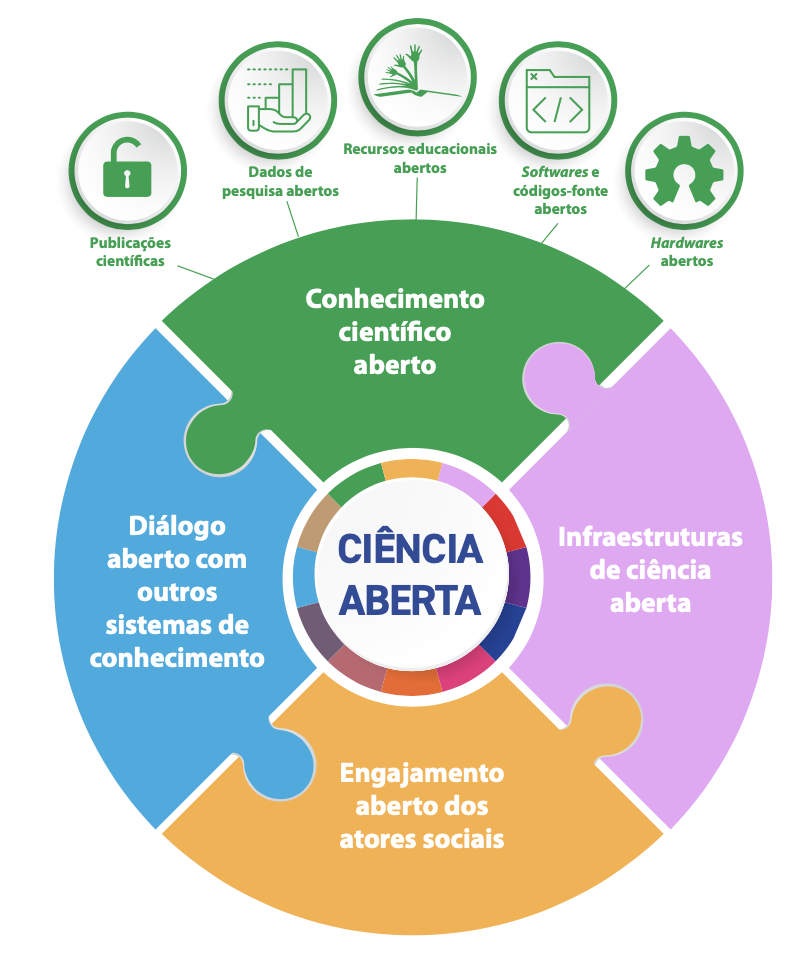
\includegraphics[scale=0.6]{JAI 2023/figures/unesco_OS.png}
    \caption{Definição de Ciência Aberta~\cite{unesco:2021}.}
    \label{fig:unesco}
\end{figure}

No contexto deste capítulo, que trata especificamente sobre princípios e práticas do \RS, colocamos ênfase em conceitos do \textit{conhecimento científico aberto}, que versa sobre o 
acesso aberto a publicações científicas, dados de pesquisa, software de pesquisa, que estejam disponíveis em domínio público ou sob direitos autorais e licenciados sob uma licença aberta. Conceitos relacionados aos demais pilares estão descritos na Recomendação da UNESCO sobre Ciência Aberta~\cite{unesco:2021}.

Consideramos que o termo \textit{Ciência Aberta} designa a \textit{prática da Ciência} de forma que outros possam \textit{colaborar e contribuir}, onde publicações, dados, software e outros artefatos de pesquisa estão \textit{disponíveis online e gratuitamente}, com base em termos que permitem a reutilização, redistribuição e \textit{reprodução} da pesquisa, seus dados e métodos subjacentes.
%
%A Figura~\ref{fig:open-science-map-by-foster} ilustra uma taxonomia que evidencia alguns tópicos e conceitos importantes para Ciência Aberta~\cite{pontika:2015}.

%\begin{figure}[htb]
%    \centering
%    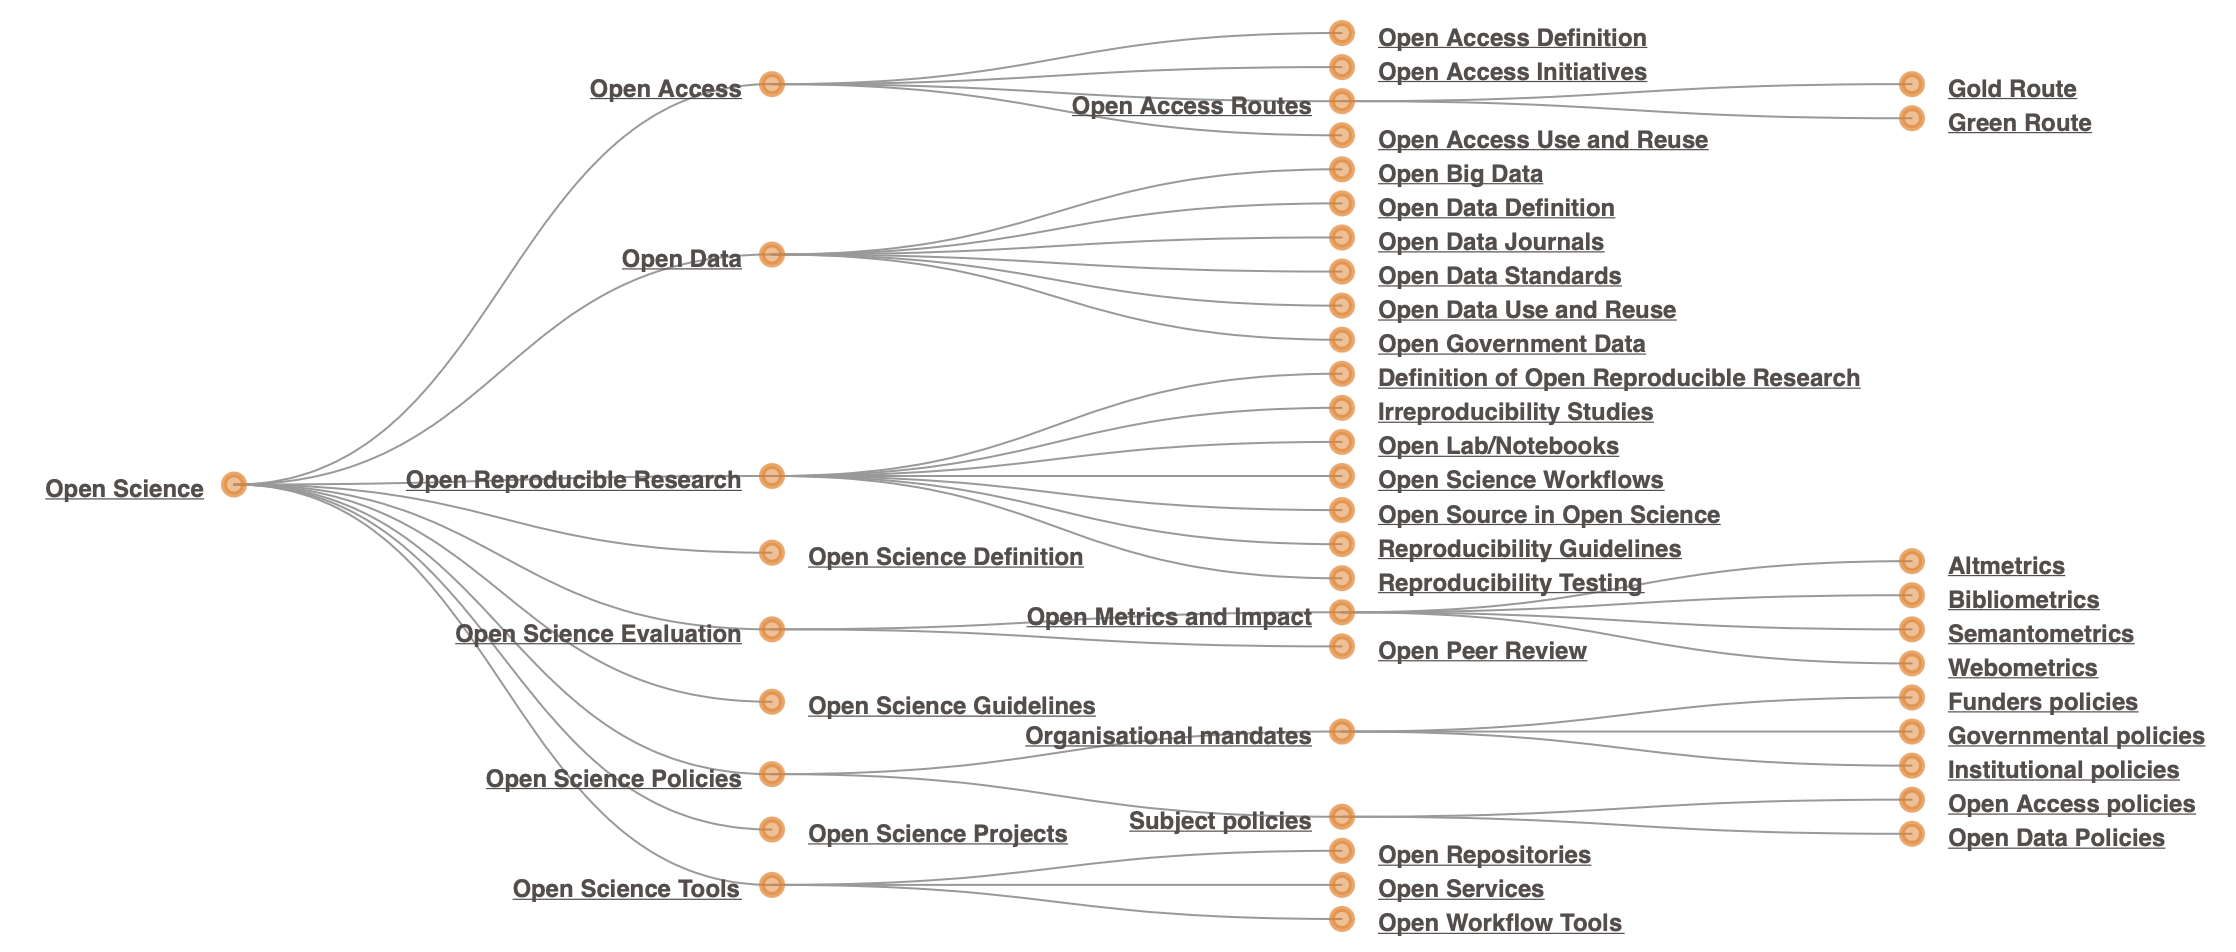
\includegraphics[scale=0.38]{JAI 2023/figures/open-science-map-by-foster.png}
%    \caption{Uma Taxonomia para a Ciência Aberta \cite{pontika:2015}.}
%    \label{fig:open-science-map-by-foster}
%\end{figure}

%Ciência Aberta no Brasil \url{https://www.unesco.org/en/fieldoffice/brasilia/expertise/open-science-brazil}

%------------------------------------------------%
%\subsection{Conceitos}

\subsection{Dados Abertos}

% Open data implies freedom to access, use and re-use for any purpose
Dados abertos estão acessíveis e disponíveis online, gratuitamente e podem ser usados, reutilizados e distribuídos desde que a fonte de dados seja atribuída.
%
Pesquisadores podem depositar os dados de sua pesquisa em um \textit{repositório de dados aberto}, para que outros possam encontrar, utilizar e construir sobre o seu trabalho~\cite{training:handbook}.
%
\textit{Metadados} ou informações sobre os dados, tais como, criador, palavras-chave, unidades, são essenciais para facilitar a descoberta de dados e 
\textit{identificadores permanentes} (PIDs) são necessários para rastrear os dados.

Um \textit{identificador de objeto digital} (DOI) é um identificador exclusivo atribuído a um conjunto de dados para garantir que os dados não sejam perdidos ou identificados incorretamente.
O DOI facilita a citação e o rastreamento do impacto dos conjuntos de dados, assim como os artigos de periódicos citados.
%
A \textit{citação de dados} deve ser considerada tão importante quanto a citação de artigos de periódicos e outros documentos científicos. 
Em geral, uma citação de dados deve incluir nome do autor/criador, data de publicação e título do conjunto de dados,  editora/organizador e DOI.

Agências de fomento à pesquisa passaram a exigir que dados coletados ou criados em projetos financiados sejam compartilhados com a comunidade em geral.
No Brasil, a Fundação de Amparo à Pesquisa do Estado de São Paulo (FAPESP) lançou as bases para a abertura de dados com a exigência, a partir do final de 2017, de Planos de Gestão de Dados quando da submissão de projetos\footnote{\url{https://fapesp.br/gestaodedados}}.

% criou um Código de Boas Práticas em Pesquisa, que, dentre outras determinações, destaca a necessidade da abertura dos procedimentos e resultados da pesquisa financiada pela Fundação, especialmente o ``registro, conservação e acessibilidade de dados e informações'', sempre considerando questões éticas ou legais

Em geral, a organização de dados de pesquisa abertos é temática. 
O World Ocean Database (WOD)\footnote{\url{https://www.ncei.noaa.gov/products/world-ocean-database}} é a maior coleção do mundo de dados abertos de perfis oceânicos uniformemente formatados, com controle de qualidade e disponíveis ao público. Os conjuntos de dados (\textit{datasets}) submetidos recebem um número de acesso (\textit{Accession Number}). Usuários podem utilizar o número de acesso para consultar o Geoportal do \textit{National Centers for Environmental Information (NCEI)} e obter uma cópia exata dos dados originais e seus metadados.

%Boyer, T.P., O.K. Baranova, C. Coleman, H.E. Garcia, A. Grodsky, R.A. Locarnini, A.V. Mishonov, C.R. Paver, J.R. Reagan, D. Seidov, I.V. Smolyar, K. Weathers, M.M. Zweng,(2018): World Ocean Database 2018. A.V. Mishonov, Technical Ed., NOAA Atlas NESDIS 87. \url{https://www.ncei.noaa.gov/sites/default/files/2020-04/wod_intro_0.pdf}.

\subsection{Acesso Aberto}

%Acesso online e gratuito a conteúdo científico revisado por pares com direitos autorais limitados e restrições de licenciamento. [FOSTER]

Uma das formas mais comuns de divulgar os resultados de uma pesquisa científica é escrever um artigo e publicá-lo em periódicos, anais de conferências ou livros. 
%
Em geral, tais publicações são disponibilizadas ao público mediante pagamento, através de uma assinatura institucional ou de forma individual. Entretanto, nos últimos anos, as taxas praticadas pelas editoras têm sido altíssimas, inviabilizando o amplo acesso ao conhecimento científico e criando desigualdades regionais.

O Movimento de Acesso Aberto\footnote{\url{https://en.unesco.org/open-access/open-access-movement}} surgiu com o propósito de
tornar todos os resultados de pesquisa disponíveis para o público sem quaisquer restrições. 
As duas estratégias mais conhecidas para publicação de artigos científicos promovem modelos alternativos, visando a ampla divulgação e redução de custos. 

\subsection*{Publicação em repositórios institucionais ou temáticos}

Esta estratégia recomenda o auto-arquivamento por pesquisadores, que depositam e divulgam os seus artigos em repositórios abertos -- institucionais ou temáticos. 
% Estratégia: fornecer ferramentas e assistência aos acadêmicos para o depósito dos seus artigos com revisão por pares em repositórios eletrônicos abertos. 

No Brasil, várias universidades oferecem repositórios institucionais para que pesquisadores depositem a sua produção acadêmica. 
Por exemplo, o Repositório Institucional da Universidade Federal da Bahia (RI-UFBA)\footnote{\url{https://repositorio.ufba.br}} é um serviço de informação científica que utiliza o DSpace\footnote{\url{https://github.com/DSpace}}, um pacote de software livre e de código aberto, para gerenciar e a disseminar a produção acadêmica da UFBA em consonância com as recomendações da Ciência Aberta. 

Nos últimos anos, pesquisadores têm depositado uma versão de seus artigos pré-impressão (\textit{preprints}) em repositórios abertos temáticos, por exemplo, o arXiv\footnote{\url{https://arxiv.org}}. 
O \textit{Computing Research Repository (CoRR) - arXiv}\footnote{\url{https://arxiv.org/archive/cs}} hospeda artigos da área de Computação.

% NÃO - O \textit{Open Science Repository}\footnote{\url{http://www.open-science-repository.com}} é um projeto para publicar trabalhos de pesquisa originais em acesso aberto, o que significa que os leitores não precisam pagar para ter acesso ao conteúdo completo da pesquisa. Pesquisadores de todos os campos da ciência podem publicar artigos originais e outras comunicações acadêmicas.

\subsection*{Publicação em periódicos e revistas de acesso aberto} 

Esta estratégia recomenda o desenvolvimento de uma nova geração de periódicos que usam os direitos de autor e outros instrumentos para garantir o acesso aberto permanente a todos os artigos que publicam. Os periódicos de acesso aberto permitem o acesso gratuito aos leitores e autorizam a reutilização da maioria dos seus conteúdos quase sem restrições.
%
Vários periódicos têm sido criados com acesso aberto, por exemplo, a série \textit{PeerJ}. %\footnote{\url{https://peerj.com}}. 
O periódico \textit{PeerJ Computer Science}\footnote{\url{https://peerj.com/computer-science/}} é o veículo voltado para a área de Computação.

O \textit{Journal of Open Source Software} (JOSS)\footnote{\url{https://joss.theoj.org}}
é um periódico de acesso aberto voltado para a publicação de \textit{pacotes de software de pesquisa}, sem taxas de processamento de artigos ou taxas de assinatura~\cite{joss:2017}.
O JOSS possui um processo formal de revisão por pares para melhorar a qualidade do software submetido. Após a aceitação no JOSS, o artigo recebe um DOI e é listado no site do JOSS.


% Closed access is the traditional form of scientific publishing. In this mode, once an article is published, it no longer belongs to you. You can share article copies privately, but may not make them public. 
%
% Green open access allows you to share either the reviewed (post-print) or originally submitted (pre-print) manuscript of your paper to certain websites or repositories. Often there is an embargo period of 6-24 months before sharing is allowed to give the publisher the chance to recoup its investment (certain journals may also allow sharing the published version after an embargo period). 
%
%Gold open access publishing retains the copyright to the author. This makes the final paper free to download for anyone from the journal website and allows unrestricted sharing online. Since the publisher in this case does not get to charge the reader, it is often the author who has to pay a fee for publishing. There is also a caveat: many closed-access journals offer unrestricted access to a specific article against a fee from the author. This so-called “hybrid gold open-access” mode is not encouraged by many scientific institutions because they essentially have to pay the publisher twice – once for the subscription and on top of it – a publication fee. 

\subsection*{Publicação de Artefatos de Pesquisa}

Além dos artigos científicos, repositórios de acesso aberto também são úteis para preservar e compartilhar \textit{outros produtos e artefatos} gerados durante a pesquisa científica,  permitindo que outros pesquisadores possam estudá-los e trabalhar com eles.
%
Há diversos repositórios abertos internacionais, dentre eles, 
Digital Commons, DSpace e  Wikimedia Commons~\cite{abdo2015direccoes}.
%, EPrints, Dataverse, GenBank, CERN Open Hardware Repository, iGem Registry of Standard Biological Parts, Addgene, Central, EuroBioBank, e Cooperative Human Tissue Network
%No Brasil, há alguns repositórios temáticos, como o SinBiota\footnote{\url{http://sinbiota.biota.org.br/about}}.
%
Exemplos de repositórios abertos conhecidos pela comunidade brasileira são Zenodo, Figshare e OSF.

\textit{Zenodo}\footnote{\url{https://zenodo.org}} é um repositório aberto de uso geral, criado para apoiar os movimentos de acesso aberto e dados abertos na Europa.
Pesquisadores podem depositar artigos, conjuntos de dados, \RS, relatórios e quaisquer outros artefatos digitais relacionados à pesquisa. Para cada envio, um identificador de objeto digital persistente (DOI) é criado, o que torna os itens armazenados facilmente citáveis.
%
\textit{Figshare}\footnote{\url{https://figshare.com}} permite a hospedagem de grandes quantidades de dados que aparecem em artigos online.
%
O \textit{Open Science Framework (OSF)}\footnote{\url{https://osf.io}} é uma ferramenta
de código aberto para o gerenciamento de projetos que oferece suporte aos pesquisadores durante todo o ciclo de vida do projeto de pesquisa. 
É também uma ferramenta de colaboração, que dá suporte ao trabalho em equipe em projetos de forma privada ou torna todo o projeto e seus artefatos publicamente acessíveis para ampla divulgação. 
%OSF permite conexões com outras ferramentas científicas que os pesquisadores usam, agilizando seu processo, aumentando a eficiência e promovendo a transparência e reprodutibilidade científicas.

%provide community resources and capabilities to enable scientists and workflow systems developers to discover software products, related efforts, events, technical reports, etc. and engage in community-wide efforts to tackle workflows grand challenges
% Use collaborative tools such as GitHub and the Open Science Framework for increased collaboration for the research process, writing/authoring, and sharing your research outputs.


%\subsection{Revisão por Pares Aberta}
\begin{comment}
% Peer review is a complex process.
% The main idea behind open peer-review is to enable a fully transparent and author-driven process
% Researchers can use open reviews to their advantage and they can get credit for the reviews they perform

A Revisão por Pares Aberta (\textit{Open Peer Review}) é um processo de validação por pares realizado abertamente na Internet, em que alguns aspectos do processo de revisão são abertos à comunidade de pesquisa ou ao público. Os manuscritos são disponibilizados pelos autores imediatamente antes dos procedimentos formais de revisão por pares. 
No processo, autores e revisores estão cientes da identidade um do outro e os relatórios de revisão são abertos e acessíveis e são publicados juntamente com o artigo disponibilizado. Uma entidade organizacional diferente do local de publicação dá suporte ao processo de revisão.
A comunidade em geral pode contribuir para o processo de revisão (pesquisadores ou o público em geral).
\end{comment}

\subsection{Pesquisa Reprodutível Aberta}

A \textit{Pesquisa Reprodutível Aberta} é definida como ``o ato de praticar Ciência Aberta e a provisão de oferecer aos usuários acesso gratuito a elementos experimentais para reprodução de pesquisas'' \cite{training:handbook}.
%
A Reprodutibilidade é definida como a capacidade de investigadores independentes de tirar as mesmas conclusões de um experimento seguindo a documentação compartilhada pelos pesquisadores que originalmente realizaram a pesquisa.
A reprodutibilidade na pesquisa científica aumenta a credibilidade da pesquisa.

Na pesquisa reprodutível aberta, os dados abertos fornecem os insumos necessários para que os pesquisadores validem e reproduzam os resultados uns dos outros. 
Entretanto, o acesso aos dados de pesquisa e artigos científicos não é mais suficiente para assegurar a reprodutibilidade na pesquisa. 
É importante definir e documentar os fluxos de trabalho (\textit{workflows}) da pesquisa.

O pesquisador deve pensar em reprodutibilidade desde o início de sua pesquisa, documentando e compartilhando cada etapa do fluxo de trabalho -- desde a coleta ou acesso aos dados, filtragem  e limpeza, até a análise de dados -- de modo a criar um roteiro ou guia para que ele e outros pesquisadores possam seguir.  A documentação deve incluir e justificar decisões importantes, por exemplo, excluir certos valores ou ajustar certos parâmetros do modelo.
O uso de software de {\em workflow} permite que cientistas automatizem e repliquem facilmente os fluxos de trabalho
em cada etapa de coleta e análise de dados.

A iniciativa {\em Workflows Community}\footnote{\url{https://workflows.community/}} compartilha recursos fornecidos pela comunidade de plataformas de software de coleta e análise de dados em pesquisa científica. 
%
Ferramentas como o Nextflow\footnote{\url{https://nextflow.io}} orquestram, de maneira simplificada e aberta, {\em pipelines} de dados de maneira portável e escalável, com suporte a instalação em uma variedade de plataformas, incluindo computadores locais,  infrastruturas como HPC e Kubernetes, e de Computação em Nuvem como AWS, Azure e Google Cloud. 
%
Outras soluções, por exemplo, o {\em Guix Workflow Language (GWL)}\footnote{\url{https://guixwl.org}} 
oferecem extensões de apoio a computação científica para a linguagem declarativa de pacotes do GNU Guix, permitindo combinar pacotes Guix com workflows científicos.

Na Ciência Aberta, além dos dados abertos e fluxos de trabalho documentados, o software também é reconhecido como elemento experimental e parte fundamental do método científico.

%-------------------%
\begin{comment}

\begin{table}[tbp]

\begin{tcolorbox}[colback=white,title=Definições da Ciência Aberta]
\begin{description}
    \item[Dados Abertos.] Dados online, gratuitos e acessíveis que podem ser usados, reutilizados e distribuídos desde que a fonte de dados seja atribuída.
\end{description}
\begin{description}
    \item[Acesso Aberto.] Acesso online e gratuito a conteúdo científico revisado por pares com direitos autorais limitados e restrições de licenciamento.
%    \item[Revisão por pares Aberta.] Processo de validação por pares realizado abertamente na Internet.
    \item[Código Aberto.]
    Software amplamente acessível para uso, seja como software livre, gratuito ou comercial.
    \item[Software Livre.]
    Software disponibilizado com licenças atribuídas que permitem ao usuário leitura, execução, adaptação e distribuição.
    \item[Pesquisa Reprodutível Aberta.]  
    Ato de praticar Ciência Aberta e oferecer acesso gratuito a elementos experimentais para reprodução de pesquisas.
\end{description}
\end{tcolorbox}

\end{table}
\end{comment}

%-------------------------------------%

\subsection{Código Aberto}

Na Ciência Aberta, 
\textit{Código Aberto} é o termo usado para caracterizar software amplamente acessível para uso, seja como software livre, gratuito ou comercial~\cite{training:handbook}.
%
``Aberto'' pode ter dois significados diferentes: apenas o código-fonte está disponível em código aberto ou o software é desenvolvido de forma aberta~\cite{herman:2022}.

Projetos de Software Livre disponibilizam o código-fonte e são 
desenvolvidos de forma aberta, com licenças de software atribuídas que permitem ao usuário leitura, execução, adaptação e distribuição.
%
Alguns pesquisadores consideram que o software livre é um pré-requisito para a Ciência Aberta~\cite{flach:sbc:2021,10.12688/f1000research.23224.2}.

Uma outra forma de compartilhar código aberto são os \textit{notebooks}, fundamentados na Programação Letrada (\textit{Literate Programming})~\cite{knuth:84}). 
Um programa letrado é uma combinação de documentação e programa-fonte organizada de modo que possa ser lida por pessoas.
Ferramentas de programação letrada extraem do arquivo uma documentação legível e um programa-fonte compilável. 
\textit{Notebooks} Jupyter\footnote{\url{https://jupyter.org}} são usados para análise exploratória e preparação de dados, treinamento e teste dos modelos. O código escrito em um \textit{notebook} pode ser extraído e empacotado como um módulo ou biblioteca Python para posterior reutilização.

% The notebooks on GitHub are the actual ‘scholarship’
%sharing the code through interactive notebooks,
%a browser-based and interactive notebook with support for code, rich text, mathematical expressions, inline plots and other rich media
%an ideal platform to support open and reproducible research.
%- The notebooks on GitHub are the actual ‘scholarship’

% Considere usar ferramentas de código aberto. Isso permite que qualquer pessoa reproduza pesquisas com mais facilidade, e ajuda a identificar quem tem a licença certa para o software usado.

%Diferentemente de desenvolvedores de software comercial tradicionais, provavelmente alinhados com desenvolvedores em projetos de código aberto, os programadores de software aberto não têm clientes e os requisitos do software raramente são congelados.




%------------------------%

% to provide guidance to the research enterprise and its stakeholders as they build strategies for achieving open science and take the next steps. In order to frame the issues and possible actions, the committee developed the concept of open science by design, defined as a set of principles and practices that fosters openness throughout the entire research life cycle
%National Academies of Sciences, Engineering, and Medicine. 2018. Open Science by Design: Realizing a Vision for 21st Century Research. Washington, DC: The National Academies Press. https://doi.org/10.17226/25116.

%In recent years “Alternative Metrics” or altmetrics have become a topic in the debate about a balanced assessment of research efforts that complement citation counting by gauging other online measures of research impact, including bookmarks, links, blog posts, tweets, likes, shares, press coverage and the like.

%Normalmente, um “projeto” no OSF, ou em qualquer outro repositório, será associado a um ou mais estudos conforme relatado em um artigo. A estrutura da pasta dependerá naturalmente do que você deseja compartilhar. Não existe um padrão comumente aceito. As pastas podem, por exemplo, ser organizadas por estudo, por tipo de arquivo (scripts de análise, dados, materiais, papel) ou tipo de dados (bruto x processado).


%------------------------------------------%
% \subsection{O Papel do Software na Ciência}
% \label{sec:software:ciencia}
% \subsection{A Importância do Software de Pesquisa}
%------------------------------------------%
\section{Software na Ciência} \label{sec:software:ciencia}

Na Ciência moderna, os dados de pesquisa (\textit{research data}) dependem, de modo crescente, do ambiente de software em que foram criados, gerenciados, analisados e apresentados. 
Resultados digitais da pesquisa, como publicações científicas e conjuntos de dados abertos, não podem ser visualizados ou usados sem o software apropriado. 
%Ainda, software usualmente tem um curto ciclo de vida, rapidamente se tornando inútil se não for apropriadamente mantido e sustentado. 

Muitas instituições, grupos e pesquisadores 
%(incluindo o UK’s Software Sustainability Institute \footnote{\url{http://www.software.ac.uk}}) 
reconhecem que todo o software desenvolvido no contexto de uma pesquisa científica deve ser considerado um resultado de pesquisa \cite{jay_software_2021} e que 
a boa prática científica exige que o software mencionado em publicações científicas seja mantido para reprodutibilidade e verificação de resultados científicos.
%
O Manifesto do Código da Ciência (\textit{Science Code Manifesto})\footnote{\url{http://sciencecodemanifesto.org/}} destaca a importância do software usado ou desenvolvido \textit{durante} a pesquisa científica:
\begin{quote}
   ``Software é um produto de pesquisa essencial e o esforço para produzir, manter, adaptar, e fazer a curadoria do código deve ser reconhecido. O Software é parte de outras contribuições científicas vitais além de artigos publicados.''  
\end{quote}

%------------------------------------%

\subsection{Software como Instrumento}

%Software e hardware especializados são usados para a captura, processamento, manipulação, registro, relatório, armazenamento ou recuperação de calibração ou dados de teste. Neste contexto, o software de computador deve estar documentado e adequado para uso.

% Instrumentos científicos contém uma quantidade significativa de software
Software é usado como parte integral de muitos instrumentos científicos, por exemplo, telescópios e microscópios. 
%Instrumento pode ser tanto físico quanto virtual; por exemplo, 
Outras vezes, o próprio software é o instrumento, gerando dados de pesquisa, validando dados de pesquisa, ou testando hipóteses. 
Isto inclui métodos computacionais ou modelos e simulações, por exemplo, modelos climáticos, modelos baseados em agentes em ciências sociais, simulação de hardware, dentre outros \cite{nieuwpoort_defining_2023}.

\subsection{Software como Contribuição Científica}

Software tornou-se parte fundamental de um ecossistema científico que engloba recursos, publicações~\cite{howison2011scientific} e 
possui a particularidade de se relacionar com o sistema econômico de reputação científica, especialmente com o seu modelo de publicações, influenciando e sendo influenciado diretamente pelo impacto de suas publicações \cite{howison2015understanding}.

A Figura~\ref{fig:scientific-reputation-diagram} mostra que a \textit{Pesquisa} conduzida por um ou mais pesquisadores pode gerar \textit{Publicações científicas} com resultados para a área do conhecimento, e também pode produzir \textit{Software} e \textit{Publicação do software}~\cite{howison2015understanding}.
As publicações científicas podem receber \textit{Citações} dos pares, o que contribui para aumentar a \textit{Reputação} acadêmica dos pesquisadores e, eventualmente, retroalimentar o sistema na forma de novos \textit{Recursos} para a pesquisa.

\begin{figure}[tb]
  \center
  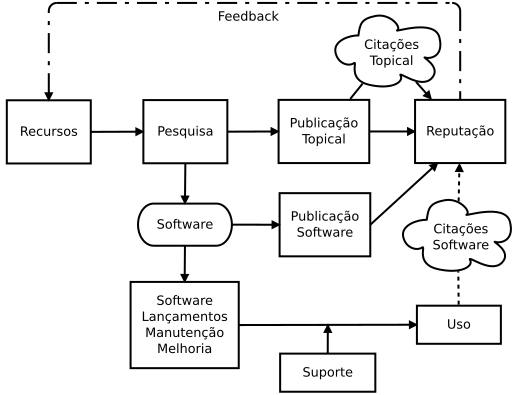
\includegraphics[scale=0.4]{figures/scientific-reputation-diagram.png}
  \caption{Uma visão dos incentivos de reputação num contexto misto entre Ciência e práticas de software de pesquisa.~\cite{howison2011scientific}}
  \label{fig:scientific-reputation-diagram}
\end{figure}

A Figura~\ref{fig:scientific-reputation-diagram} também relaciona  \textit{Software} a \textit{Lançamentos, Manutenção e Melhoria}
que exigem \textit{Suporte} e levam à disponibilização do software para \textit{Uso}.
Entretanto, não há uma ligação direta e explícita entre a publicação do software e eventuais citações ao software. As setas tracejadas sugerem que o \textit{Uso} do software pode gerar citações ao software e que estas podem influenciar de modo diferente (ou mesmo não influenciar) a reputação dos pesquisadores.
Este problema pode ser explicado pela falta de padronização da citação de software e prática frequente de ``citar'' apenas uma URL que leva a um local onde o software pode ser encontrado. 
  
A citação de software permite aos desenvolvedores receber reconhecimento e crédito pelo seu trabalho, além de facilitar a rastreabilidade e replicação dos resultados. Também contribui para a visibilidade e a colaboração na comunidade científica, fortalecendo a sustentabilidade técnica do software. No entanto, a importância do software na pesquisa ainda é subestimada, e o software é tratado como um recurso de apoio ou ferramenta, e não como uma contribuição científica em si. 
%
No ecossistema da Ciência Aberta, o software de pesquisa deve ser citável e reconhecido como uma valiosa contribuição da pesquisa científica, tão importante quanto os artigos publicados, dados e metadados.  No entanto, esforços e incentivos são necessários para que os créditos para o software de pesquisa se tornem mais específicos e rastreáveis na Ciência.

\subsection{\textit{Better Software, Better Research}}

% Artigo ``Better Software, Better Research''~\cite{goble2014better}.
% The continued development of science is partly dependent on improvements in research software. Despite the reliance on software in academia, professional practices for its development too often lag behind those in the commercial sector.

%The pressure on researchers to rapidly publish new results without the need to develop professional quality code results in fragile academic research software, generally not sustainable or usable beyond the lifetime of a given project. As a result, the research community fails to benefit from their research's potential impact fully.

Pesquisadores sofrem uma intensa e constante pressão para publicar novos resultados rapidamente sem a devida cobrança sobre a necessidade de desenvolver código de qualidade. Como consequência, o software desenvolvido durante a pesquisa tende a não ser sustentável ou usável além da duração da pesquisa ou dos recursos que a  financiam, e impede a comunidade científica de aproveitar plenamente o seu potencial impacto em pesquisas futuras.

%\subsection{Histórico} 
Em 2016, inspirada pelo artigo 
\textit{Better Software, Better Research}~\cite{goble2014better}, 
o workshop \textit{Dagstuhl Perspectives}~\cite{goble_et_al:DR:2016:6755} reuniu ativistas, especialistas e interessados em discutir sobre o software produzido no contexto acadêmico e sua qualidade, na perspectiva de grupos de pesquisa que (i)~consomem ou produzem software como saída do processo científico, ou (ii)~consomem ou produzem software como um dos componentes dos métodos de pesquisa.

Dentre os resultados principais e com base em dados sobre o crescimento no uso de software em pesquisas científicas,
o workshop identificou seis áreas no ecossistema de software de pesquisa que merecem atenção: 
\textit{crédito ao software}, tornando-o rastreável nas pesquisas científicas; \textit{herança cultural}, ou preocupação com as implicações das escolhas tecnológicas; \textit{princípios FAIR para software} (discutidos na Seção 3.4.3); \textit{financiamento} de atividades de desenvolvimento e manutenção de software; \textit{políticas e e práticas} para incentivar a colaboração, a transparência e o compartilhamento de conhecimento entre os pesquisadores e instituições; e necessidade de \textit{treinamentos} para pesquisadores e outros atores envolvidos com o desenvolvimento de software para uso na pesquisa.

Sobre treinamentos, o workshop recomendou que os mesmos devem cobrir diversos tópicos relacionados ao desenvolvimento de software e níveis de prática, e que cursos oferecidos por alguns institutos, por exemplo, \textit{Carpentries}, devem ser estimulados e apoiados.
%
Práticas centrais para manutenibilidade do software devem ser apresentadas, incluindo controle de versão, padrões de codificação, revisão de código, programação em par, testes, cobertura de código, integração contínua, refatoração e documentação. 
%
Outros tópicos também devem ser considerados, por exemplo, quão aberto é um software, se é desenvolvido por uma comunidade ou por um indivíduo, quão ativa é a manutenção do software (correção de \textit{bugs} e criação de novas funcionalidades) ou disponibilidade de recursos diversos~\cite{sufi_report_2020}.

%
%A próxima seção apresenta conceitos e atributos do \textit{software de pesquisa} \cite{gruenpeter_morane_2021_5504016} e destaca a sua importância no ecossistema da Ciência Aberta.

\section{Software de Pesquisa}
\label{section:researchsoftware}

\subsection{Definição}
% definition of Research Software as a separate metaphor of software in research.

O termo \textit{software de pesquisa} foi criado para designar, de modo abrangente, o software \textit{utilizado} durante a pesquisa científica, incluindo o software de terceiros usado para coleta, processamento e análise de dados~\cite{allen_et_al:DM:2017:7146}.
%
%Additional software components (e.g., operating systems, libraries, dependencies, packages, scripts, etc.) that are used for research but were not created during or with a clear research intent should be considered software in research and \textbf{not} Research Software.
%
No contexto de avaliação de qualidade do software de pesquisa,
\cite{gruenpeter_morane_2021_5504016} adotam uma visão mais restrita, e consideram que sistemas operacionais, bibliotecas, dependências, pacotes e \textit{scripts} utilizados na pesquisa científica, mas que não foram criados durante ou com uma intenção de pesquisa clara, são \textit{software usado na pesquisa} mas \textit{não são software de pesquisa}.
% RS should be FAIR! \cite{gruenpeter_morane_2021_5504016}.
% Esta definição erviu para definir o escopo e guiar o trabalho sobre FAIR4RS, identificando os artefatos de software que poderiam ser avaliados segundo tais princípios.
%
No restante deste capítulo, adotaremos a visão de software de pesquisa de~\cite{gruenpeter_morane_2021_5504016}: 

\textit{Software de Pesquisa é o software desenvolvido durante o processo de pesquisa e inclui (mas não está limitado a) código-fonte, algoritmos, \textit{scripts}, fluxos de trabalho computacionais e executáveis.} 

%\subsection{Caracterização}

O \RSw é parte integrante do ecossistema de pesquisa moderno,
sendo amplamente utilizado nas Ciências e Engenharias para gerar resultados que servem como evidência em publicações científicas. 
Em geral, devido à complexidade em desenvolver software e ao conhecimento de domínio especializado necessário, os próprios pesquisadores desenvolvem o \RSw ou estão intimamente envolvidos com o seu desenvolvimento~\cite{carver:icse:2007}.
% Carver survey identifies the steps involved in developing scientific software (i.e. the life cycle, the workflows, technical challenges, and organizational challenges).

Há várias preocupações relacionadas à \textit{natureza} e à \textit{qualidade} do \RS. 
%
Como artefato digital, ele pode assumir muitas formas, por exemplo, um \textit{script} shell bash, com apenas 50 linhas para manipular e filtrar arquivos, um conjunto de \textit{scripts} R de 100 linhas para análise de dados, 10.000 linhas de código Java para software de análise de dívida técnica ou 50.000 linhas de C++ para análise de imagens médicas. 
%Pode ser escrito em linguagens de \textit{script} como Unix shell, Python, R ou MATLAB ou em linguagens de programação como C, C++, Fortran ou Java. 
%
% Ele pode ser hospedado e distribuído de várias maneiras, incluindo repositórios abertos digitais (GitHub, BitBucket, GitLab), projetos como Software Heritage, websites de projetos de pesquisa, pastas FTP, e redes para arquivamento e gerenciamento de artefatos, por exemplo, CRAN (Comprehensive R Archive Network), CPAN (Comprehensive Perl Archive Network), PyPI (Python Package Index), e NPM (Node Package Manager).

%Figura~\ref{fig:mindmap} ... De onde veio mesmo? % (nao sei de onde veio -- joenio)
%\begin{figure}[tbp]
%    \centering
%    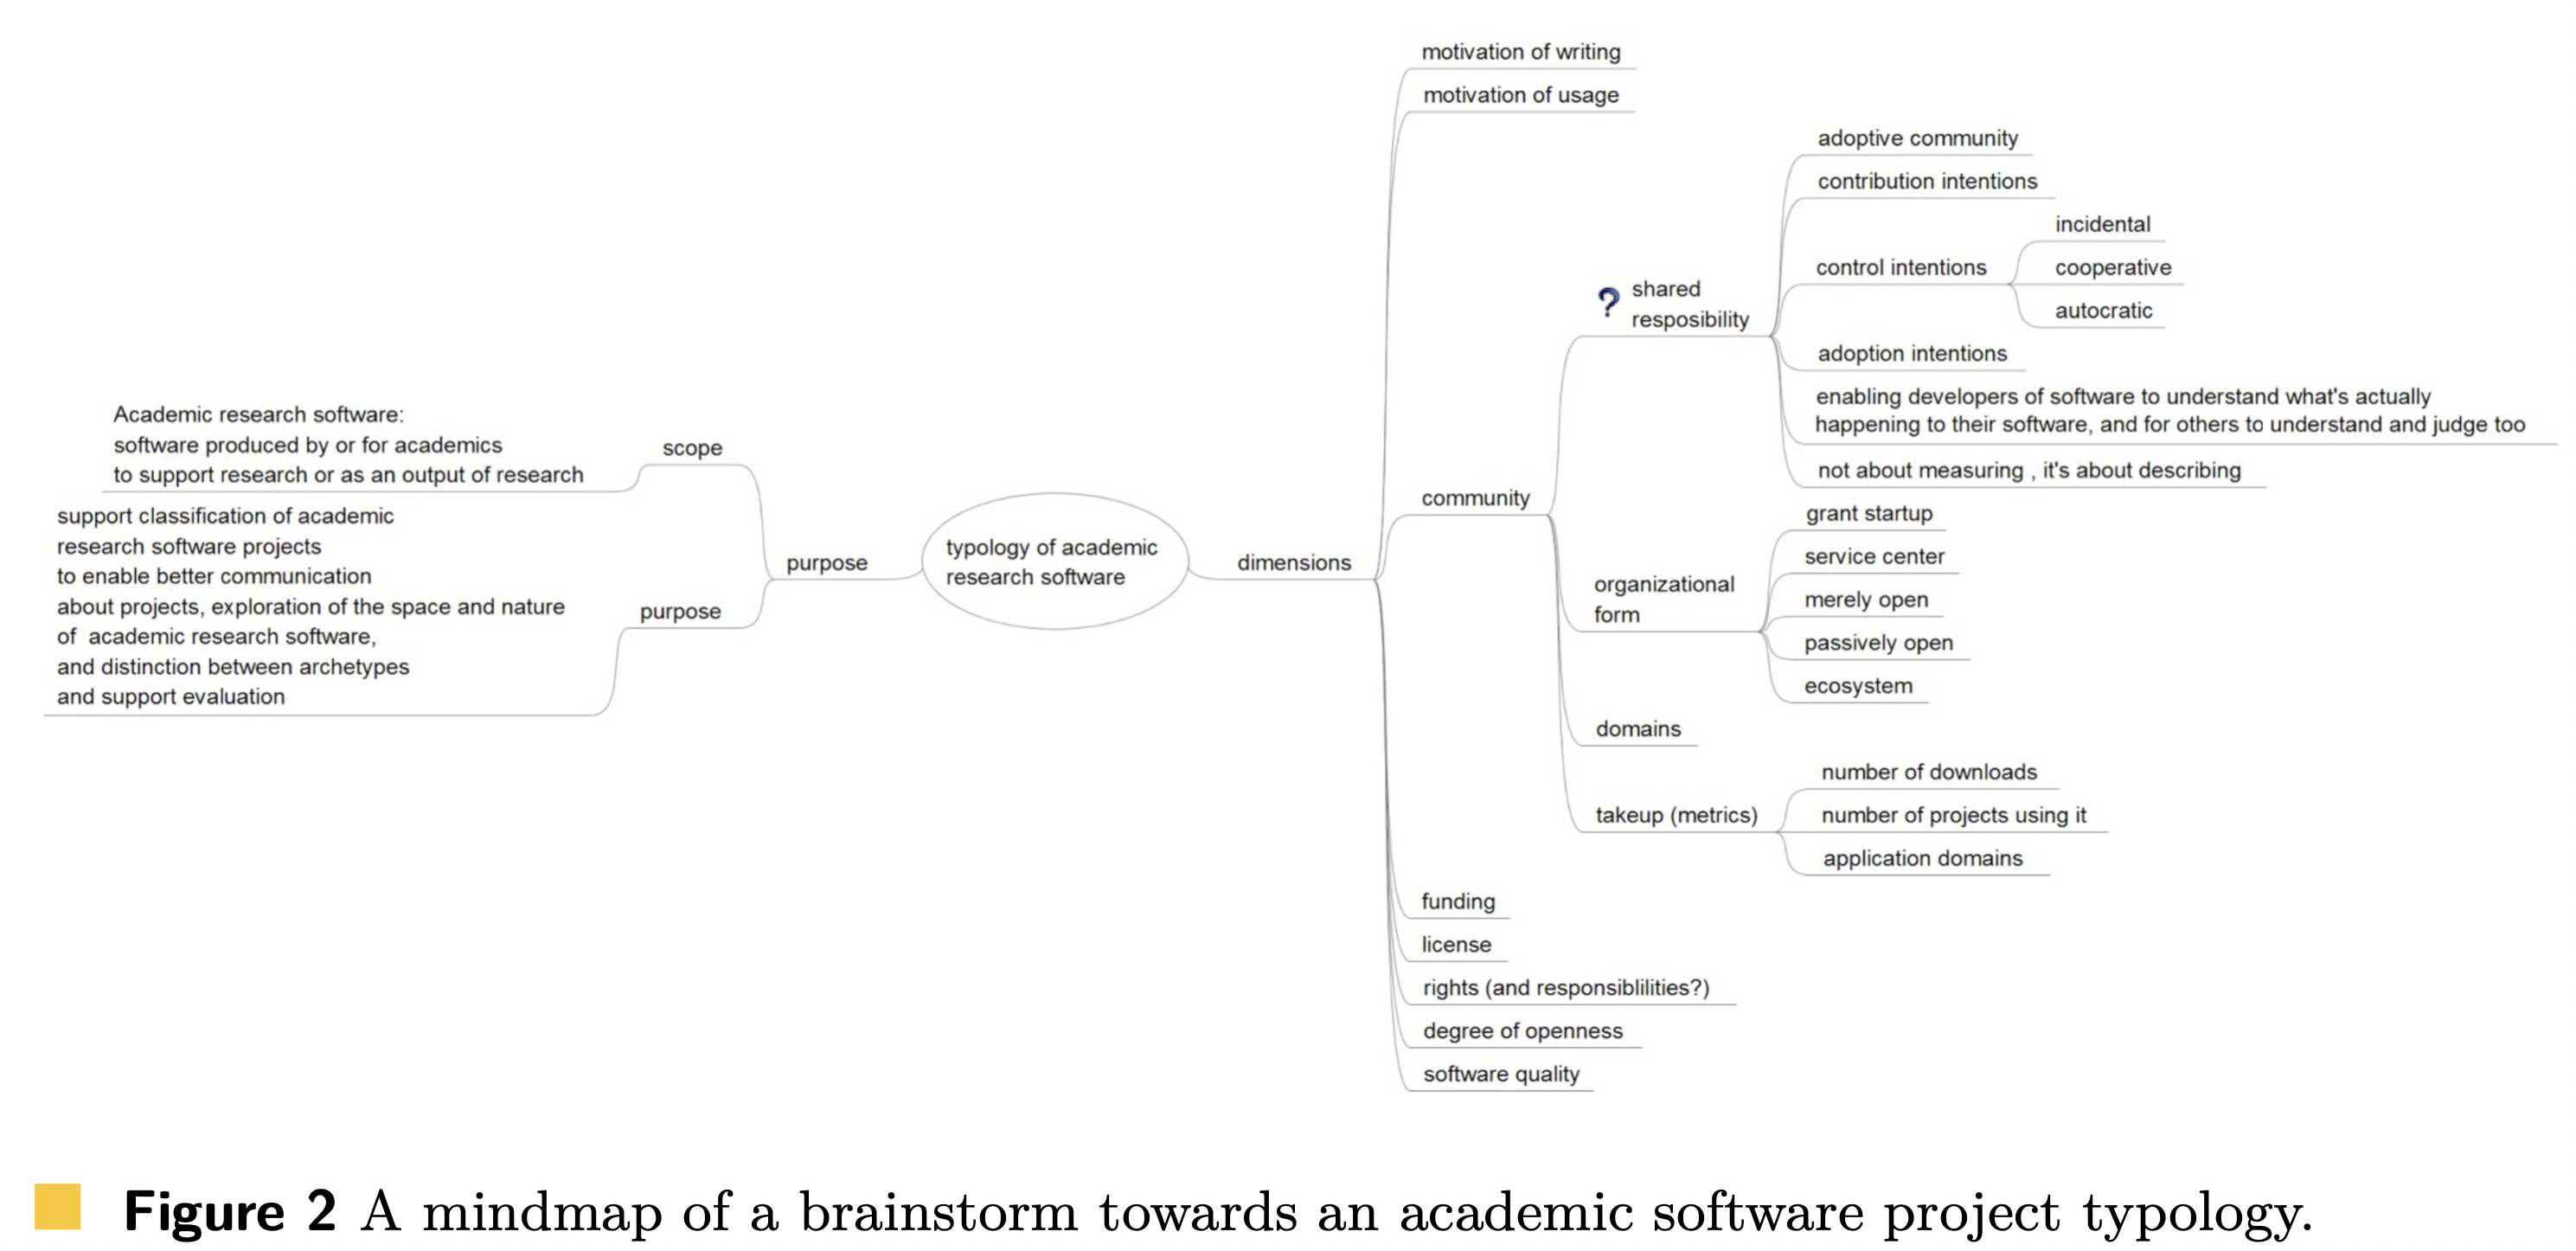
\includegraphics[scale=0.28]{JAI 2023/figures/RS-typology.png}
%    \caption{Figura do mindmap -- ontologia [CITAR]}
%    \label{fig:mindmap}
%\end{figure}
%
Como produto de software, o \RSw deve considerar alguns atributos de qualidade desejáveis.
%, sob diferentes perspectivas, por exemplo, usuários, desenvolvedores, e outros interessados. 
Por exemplo, é desejável que o \RSw seja confiável, eficiente, fácil de usar, fácil compreender, testar, reparar, estender ou adaptar.
%Podemos considerar que tais atributos podem estar associados ao software ou ao seu processo de desenvolvimento.
% 
Em especial, há uma preocupação com a sustentabilidade do \RSw e sua influência na reprodutibilidade da pesquisa científica.

Neste capítulo, apresentamos aspectos relacionados à  sustentabilidade do \RSw e boas práticas para o desenvolvimento de software sustentável, a saber: 
registro e identificação do software, licenças de software e grau de abertura (\textit{openness}), reconhecimento e citação do software, comunidade e usuários, longevidade e manutenibilidade, aderência aos princípios FAIR para software, avaliação do \RS e sua influência na reprodutibilidade científica.

%All research software is open
%All research software is high-quality and robust
%All research software is findable, accessible, and usable & used by others (for their own research), and is cited when it is used
%All contributors to research software are recognized for their work, with good careers
%All research software is sustained as long as it is useful
%All research is reproducible

%--------------------------------------------% 
\subsection{Sustentabilidade}
\label{subsection:srs}
%--------------------------------------------% 

% O desenvolvimento sustentável atende às necessidades do presente sem comprometer a capacidade das gerações futuras de atender às suas próprias necessidades. O desenvolvimento sustentável exige esforços conjuntos para a construção de um futuro inclusivo, sustentável e resiliente para as pessoas e o planeta.

\textit{Sustentabilidade} é um dos princípios norteadores da Ciência Aberta~\cite{unesco:2021} e define que a mesma
deve se basear em práticas, serviços, infraestruturas e modelos de financiamento de longo prazo que garantam a participação igualitária dos indivíduos que produzem ciência originários de instituições e países menos privilegiados. 
As infraestruturas científicas abertas devem ser organizadas e financiadas com base em uma visão essencialmente sem fins lucrativos e de longo prazo, que aprimorem as práticas de Ciência Aberta e garantam o acesso permanente e irrestrito a todos, na medida do possível.
%
No contexto da Ciência Aberta e sua dependência 
no código aberto (Seção~3.2.5), observa-se uma preocupação crescente com a sustentabilidade do software usado ou desenvolvido durante a pesquisa, em especial, com a longevidade e disponibilidade do software, e seu impacto na reprodutibilidade científica.
%

% Desenvolvimento sustentável, definido pela Comissão Brundtland [Brundtland, 1997] trata de "satisfazer as necessidades do presente sem comprometer a capacidade das gerações futuras de atender às suas próprias necessidades".

O tema Sustentabilidade, inicialmente associado ao campo da Ecologia, agora faz parte dos interesses de outras áreas do conhecimento, ainda que adaptado às especificidades de cada uma. 
Na Ciência da Computação, a preocupação com a sustentabilidade emerge como um tópico importante em diversas subáreas, incluindo Inteligência Artificial, Computação de Alto Desempenho, Interação Humano-Computador, Computação Científica e Engenharia de Software \cite{venters_software_2021}.
Sustentabilidade é um desafio a ser enfrentado, não um problema a ser resolvido~\cite{becker_2014}.

O \textit{Manifesto de Karlskrona} para o Design Sustentável~\cite{becker_2014}
define que sustentabilidade é, em sua essência, um conceito sistêmico, multi-facetado e deve ser entendida em um conjunto de cinco dimensões:
recursos ambientais, social, bem-estar individual, prosperidade econômica e viabilidade técnica de longo prazo.

Neste capítulo, abordamos aspectos da dimensão técnica da sustentabilidade do
software~\cite{DBLP:conf/re/KehrerP18} e, de forma complementar, elementos de sua dimensão social~\cite{DBLP:journals/sigsoft/Souza23}. 
% ou questões sócio-técnicas, e 
Não trataremos de aspectos da Engenharia de Software Verde~\cite{ivan:green:2018}\footnote{A Engenharia de Software Verde leva em consideração práticas e arquitetura de software, design de hardware e \textit{data center}, o mercado de eletricidade e mudanças climáticas, visando gerar menos emissões de gases de efeito estufa e reduzir produção de carbono de uma empresa~\cite{ivan:green:2018}.}.

\subsection*{Sustentabilidade de Software}
\label{subsection:sustainability}

Na Engenharia de Software, há duas linhas de pesquisa voltadas para Sustentabilidade que se destacam: 
(i)~Sustentabilidade de Software, e 
(ii)~Engenharia de Software para Sustentabilidade (SE4S). 
%
A pesquisa sobre \textit{Sustentabilidade de Software} tem como preocupação central a capacidade do software de perdurar ao longo do tempo,
enquanto que a pesquisa relacionada a SE4S preocupa-se com
sistemas intensivos em software, como integrar a sustentabilidade em seus processos de desenvolvimento de software
e apoiar a sustentabilidade ambiental
na ampla variedade de domínios em que o software é implantado \cite{venters_software_2021}.
%
%Entre estes dois universos há ainda um grande espaço para debate e construção de um entendimento comum sobre os conceitos fundamentais de sustentabilidade e como ela se relaciona com o software, visto que não há um acordo na comunidade de software sobre a definição de sustentabilidade de software ou como ela deve ser atingida. Apesar das inúmeras contribuições para formalizar a definicao de sustentabilidade de software, o conceito continua intangível e ambíguo, com indivíduos, grupos e organizacional mantendo visões diametralmente opostas.

No que se refere à sustentabilidade de software,
a longevidade como expressão de tempo (``longo prazo'') e a capacidade de manutenção são fatores-chave para sua compreensão~\cite{venters_2018}.
%
A preocupação com a longevidade do software estende-se ao atributo de manutenibilidade, e ao modelo e processo de desenvolvimento de software adotados, que podem influenciar atributos relacionados à sustentabilidade.
A manutenibilidade é reconhecidamente uma qualidade interna fundamental de sistemas de software~\cite{iec2014iso}, 
enquanto que a sua relação com a sustentabilidade de software ainda é objeto de pesquisa na área.
%
O termo sustentabilidade propriamente dito ainda não está bem definido neste contexto, deixando espaço para diferentes interpretações, e ainda há pouca evidência ou orientação sobre processos ou modelos de desenvolvimento voltados para a sustentabilidade de software~\cite{venters_software_2021}.
%Assim, definir sustentabilidade de software como a capacidade de perdurar ou como mais uma qualidade de software ao lado de manutenibilidade ainda não se mostra suficiente.

% The relationship between software quality and software sustainability is still an open question.
De um ponto de vista puramente técnico, \cite{venters_software_2021} define sustentabilidade de software como um requisito composto, não-funcional, de primeira classe, abrangendo as medidas de alguns conceitos centrais de atributos de qualidade de software, incluindo, no mínimo, manutenibilidade, extensibilidade e usabilidade.
Na dimensão técnica, a sustentabilidade de software está relacionada às consequências de longo prazo de projetar, construir e entregar um projeto de software e se espalha por diversas áreas, dentre elas, qualidade de software e métricas, requisitos de software e arquitetura de software~\cite{DBLP:conf/re/KehrerP18,venters_software_2021}.
Por fim, sustentabilidade de software diz respeito a assegurar que o software continue funcional para seus usuários ao longo do tempo, considerando também sua manutenção, inclusão de novos recursos, reparo de \textit{bugs}, e adaptações a novos ambientes de software e hardware.

%Portanto uma possivel abordagem para definir sustentabilidade de software eh como uma medida dos atributos: manutenibilidade, extensibilidade e usabilidade.

%In the case of software this means that it must continue to be available in the future, on new platforms and meeting new needs.
%How can we ensure sustainability of scientific software? What does this mean for a particular project?

\subsection*{Software de Pesquisa Sustentável}

O \textit{Software de Pesquisa Sustentável} deve permanecer \textit{disponível e funcional} para a comunidade científica durante períodos de tempo significativos. 
Não há uma resposta geral para a questão de quanto tempo o software precisa ser sustentado ou mantido. Este período pode depender da área de pesquisa, finalidade, função, frequência de uso, e da comunidade que o desenvolveu.

Sustentabilidade de \RSw inclui o processo de desenvolvimento e manutenção de software para que o mesmo continue a cumprir seu propósito ao longo do tempo. 
%
Certamente, o \RSw sustentável precisará ser atualizado com novas funcionalidades e correções de \textit{bugs}, adaptado a novos ambientes computacionais, manter-se amigável aos seus usuários, tornar-se multiplataforma, ser testado e certificado.
Garantir que o \RSw continue executável é desafiador, sendo  mais trabalhoso e caro do que um arquivamento simples de uma versão do software.  
As alterações necessárias para que o software permaneça executável devem garantir a confiabilidade nos resultados gerados pelas versões mais antigas do software. 
Se os resultados forem diferentes, justificativas objetivas devem ser fornecidas. 

Há diversas maneiras de promover e investir na sustentabilidade do \RS, incluindo atração de desenvolvedores, suporte à comunidade de usuários, busca por financiamento ou até comercialização -- todas válidas, desde que resultem na disponibilidade de longo prazo do software para a comunidade científica. 
Espera-se que, por meio da publicação de instruções, diretrizes e outras formas de ajuda e suporte, pesquisadores sejam capazes de decidir a forma de manter o seu software sustentável.

% Sustainable software engineering (SSE)

% Sustainable software engineering [4] motive is to create reliable, lifelong software that meets the needs of user’s requirement and also tried to reducing ecological impacts; its aim is to generate better software so there is no need to compromise future generations’ opportunities.

\subsection{\textit{FAIRness}}
\label{subsection:fair:software}

%Computational research should be FAIR: Findable, Accessible, Interoperable, Reusable. [CITAR algo]
% A modified version of these principles can be usefully applied to software too:  it should be Findable, Accessible, Reusable and Extensible. [Software as Output]

Os princípios FAIR~\cite{Wilkinson2016} foram especificados para melhorar o reuso de dados de pesquisa digitais, tornando-os mais fáceis de encontrar, acessíveis, interoperáveis e reutilizáveis (\textbf{F}indable, \textbf{A}ccessible, \textbf{I}nteroperable, \textbf{R}eusable).
%
Tais princípios abordam a \textit{forma} de fornecer artefatos para a comunidade científica, mas não tratam do conteúdo funcional ou da qualidade dos artefatos~\cite{lamprecht:2020}.
%\textbf{F}indability, \textbf{A}ccessibility, \textbf{I}nteroperability, \textbf{R}eusability.
Os \textit{Princípios FAIR para Dados de Pesquisa}~\cite{Wilkinson2016}, 
incluindo quatro princípios fundamentais e 15 princípios norteadores, estabelecem que os dados de pesquisa devem ser facilmente localizáveis, acessíveis, interoperáveis e reutilizáveis. 

Segundo~\cite{chue_hong_fair_2022}, o \RSw deve seguir os princípios FAIR usados para dados abertos, considerando-se que
o software também é um artefato de pesquisa digital e, como tal, deve ser facilmente localizável, acessível, interoperável e reutilizável. 
%
Os \textit{Princípios FAIR para Software de Pesquisa} (FAIR4RS) foram definidos a partir de uma reformulação dos princípios FAIR originais para dados abertos~\cite{lamprecht:2020,chue_hong_fair_2022,barker:2022}.
É importante destacar que, diferentemente dos dados, o software não é um artefato estático e só pode ser (re)utilizado se for sustentável~\cite{lamprecht:2020}.
%
A Tabela~\ref{tab:fairness:4:rs:r} apresenta a versão mais recente dos princípios FAIR para \RS.

\textit{Projetos de Software Livre} seguem os princípios FAIR. %recomendados para \RS.
Software livre pode ser localizado em repositórios com base em identificadores e descritores, utilizando diversos critérios como palavras-chave, linguagem de programação, versão do software, entre outros. 
A acessibilidade é encorajada em software disponível em repositórios abertos, com licenças de compartilhamento explícitas e bem definidas e documentação associada. 
A definição de interfaces de programação, formatos de entrada/saída e uso de padrões promovem a interoperabilidade e o reúso por vários grupos de pesquisa.
Nessa perspectiva, as práticas usadas no modelo de desenvolvimento de software livre podem ser adotadas no desenvolvimento e evolução de \RS~\cite{flach:sbc:2021}. 
%\footnote{\url{https://www.sbc.org.br/component/flippingbook/book/53/1?page=1}}

% Fairness template
\begin{table}[htbp]
    \caption{Princípios FAIR para Software~\cite{barker:2022}.}
    \centering
    \small
    \begin{tabular}{p{1.1cm}|p{13cm}}
    \hline
    \textbf{Princ.} & \textbf{Descrição} \\ \hline
    F: & Software, and its associated metadata, is easy for both humans and machines to find.\\
    F1 & Software is assigned a globally unique and persistent identifier.\\
    F1.1 & Software components representing granularity levels are assigned distinct identifiers.\\
    F1.2 & Different versions of the software are assigned distinct identifiers.\\
    F2 & Software is described with rich metadata. \\
    F3 & Metadata clearly and explicitly include the identifier of the software they describe.\\
    F4 & Metadata are FAIR, searchable and indexable.\\ \hline
    A: & Software, and its metadata, is retrievable via standardised protocols.\\
    A1 & Software is retrievable by its identifier using a standardised communications protocol. \\
    A1.1 & The protocol is open, free, and universally implementable.\\
    A1.2 & The protocol allows for authentication and authorization procedure, where necessary. \\
    A2 & Metadata are accessible, even when the software is no longer available.\\ \hline
    %\textbf{Princ.} & \textbf{Descrição} \\ \hline
    I: & Software interoperates with other software by exchanging data and/or metadata, and/or through interaction via application programming interfaces (APIs), described through standards.\\
    I1 &  Software reads, writes and exchanges data in a way that meets domain-relevant community standards.\\
    I2 & Software includes qualified references to other objects.\\
      \hline
    R: & Software is both usable (can be executed) and reusable (can be understood, modified, built upon, or incorporated into other software).\\
    R1 & Software is described with a plurality of accurate and relevant attributes.\\
    R1.1 & Software is given a clear and accessible license. \\ 
    R1.2 & Software is associated with detailed provenance.\\
    R2 & Software includes qualified references to other software.\\
    R3 & Software meets domain-relevant community standards. \\
      \hline
    \end{tabular} \label{tab:fairness:4:rs:r}
\end{table}

%Lots of work beyond FAIR: quality, correctness, reproducibility, openness, ...

%---------------------------------------------%
%Possivel referencia para avaliar se inclui ou nao: https://www.youtube.com/watch?v=67Uc1EEVDv8&t=953s

%O uso de \textit{Software de Pesquisa} é mencionado na literatura por meio de citação formal ou informal~ \cite{smith2016software} e está estreitamente relacionado ao sistema econômico de reputação científica, uma vez que tais menções causam impacto científico direto tanto na publicação quanto no ecossistema de software de pesquisa \cite{katz2014transitive}.

%Conhecimento novo é claramente construído a partir do conhecimento passado e o sistema de citações formais tem promovido avanços significativos \cite{katz2014transitive}.
% No entanto, isso não tem funcionado tão bem para produtos digitais como o software que, muitas vezes, dependem de outro software, fragmentos de código, e algoritmos \cite{katz2014transitive}.


\begin{comment}
\begin{table}[btp]
\begin{tcolorbox}[colback=white,title=Princípios FAIR para Software]
  \begin{description}
    \item \textbf{Localizável} \textit{(\textbf{F}indable)}
    
        O Software possui um rico conjunto de metadados e um identificador único e persistente que facilita sua busca e identificação.
    \item \textbf{Acessível} \textit{(\textbf{A}ccessible)}
    
        Os metadados do Software estão organizados e especificados em um formato legível para pessoas e máquinas. O Software e metadados devem estar depositados em repositórios públicos e reconhecidos pela comunidade.
    \item \textbf{Interoperável} \textit{(\textbf{I}nteroperable)}
    
        O Software usa padrões e plataformas reconhecidos pela comunidade possibilitando a integração com outras ferramentas e sistemas.
    \item \textbf{Reutilizável} \textit{(\textbf{R}eusable)}
    
        O Software possui uma licença e documentação que permitem sua adoção e extensão por outros pesquisadores e desenvolvedores. 
    \end{description}
\end{tcolorbox}
\end{table}
\end{comment}

%-----------------------------%
\subsection{Reprodutibilidade} \label{subsection:srrs}

A \textit{Reprodutibilidade} é um dos fundamentos do método científico e um princípio norteador da Ciência Aberta~\cite{unesco:2021}.
A boa prática científica exige que os artefatos de pesquisa mencionados em publicações científicas sejam mantidos e fiquem disponíveis para escrutínio dos pares, reprodução independente e verificação de resultados.

%Qual a importância da sustentabilidade do \RS para a pesquisa reprodutível aberta?  
%Lançamentos.
Para o \RS, a submissão ou publicação de um artigo é um dos momentos em que a versão do software usada no estudo precisa ser identificada, documentada e lançada.
% 
Se houver modificações no \RS, elas precisam ser registradas, 
usando algum esquema de nomenclatura que identifique o 
\textit{<software>}, a \textit{<versão>} e o \textit{<lançamento>}.
Em geral, a versão refere-se a mudança estratégica durante a evolução do software e o lançamento refere-se a mudanças simples de serviço.

A recomendação para que pesquisadores compartilhem e permitam o acesso aos dados descritos em suas publicações científicas, não garante a reprodutibilidade da pesquisa. 
Na prática, pesquisadores devem compartilhar o código de todo o \RSw desenvolvido e fluxos de trabalho de suas pesquisas para assegurar a reprodutibilidade.
Na maioria dos casos, o arquivamento de baixo custo do software, acompanhado de documentação clara deve ser suficiente.

Diretrizes para o desenvolvimento sustentável de \RSw também podem contribuir para a condução de uma pesquisa científica reprodutível,
apresentando princípios e boas práticas da engenharia de software.
As implementações das diretrizes podem variar entre os diferentes domínios científicos, mas as implementações devem ser públicas, abertas para discussão entre os pesquisadores e continuamente adaptadas em reposta às mudanças tecnológicas e nos domínios.

%In most cases, cheap software archiving with clear documentation (including version control, etc.) should be sufficient. 
% For this aspect of software sustainability, it is urgently needed that guidelines are given to all researchers, in particular those that are still in a phase before the actual conception of new software, on coding ethics, good practices, and other guidelines to make later use easier, once the software or tools have been created. 


%---------------------------------%
\subsection{Avaliação de \RS}

Consideramos a avaliação do \RSw sob duas perspectivas: (1)~sustentabilidade ou direcionada a sua longevidade, e (2)~aderência aos princípios FAIR (\textit{FAIRness}) ou direcionada ao grau de abertura (\textit{openness}) do \RS.

%Os princípios FAIR são critérios de referência para promover e avaliar a abertura (\textit{openness}) dos dados e do software de pesquisa.

\subsection*{Sustentabilidade}

A avaliação da sustentabilidade do \RSw busca determinar se o mesmo é sustentável com base em critérios relevantes para o ecossistema científico.
Em geral, a avaliação não gera um resultado \textit{é sustentável/não é sustentável}, mas tende a 
valorizar pontos fortes do software e identificar pontos para sua melhoria. A avaliação pode considerar atributos ou práticas usadas no desenvolvimento do software para 
prover uma visão geral ou detalhada da sustentabilidade do \RS.

O Instituto de Sustentabilidade de Software (SSI)
fornece um serviço de avaliação quantitativa do software baseada em critérios relacionados a sustentabilidade, manutenibilidade e usabilidade\footnote{
O questionário do SSI para avaliação de sustentabilidade está disponível em \url{http://www.software.ac.uk/online-sustainability-evaluation.}}.
%
A avaliação é feita com base em respostas dadas a um conjunto
de perguntas simples, seguidas por explicações sobre a importância de algumas práticas e recomendações. 
O conjunto de perguntas é aplicável para \RS.

Por exemplo, para uma resposta negativa para a pergunta 
``\textit{Seu \RSw está disponível como um pacote que pode ser instalado sem compilar?}'', a avaliação oferece a recomendação geral 
``Construir software pode ser complicado e demorado. Fornecer seu \RSw como um pacote que pode ser implantado sem compilar pode economizar tempo e esforço dos usuários, especialmente se não forem desenvolvedores de software. Idealmente, deve-se observar e testar se o \RSw é compilado e executado em diversas plataformas para as quais ele oferece suporte, para então prover pacotes para sua distribuição.'' 
%, o que significa que você já terá criado pacotes que podem ser distribuídos para seus usuários.

% \textit{Seu site e documentação fornecem uma visão geral clara e de alto nível do seu software?}, \textit{Seu software está disponível como um pacote que pode ser instalado sem compilar?}, \textit{Você publica seu histórico de lançamentos, por exemplo, dados de lançamento, números de versão, principais recursos de cada lançamento, etc., em seu site ou em sua documentação?},  \textit{Você tem um conjunto de testes automatizados para seu software?} ou \textit{Há uma citação recomendada para seu software?}.

Em nossa pesquisa, a avaliação de sustentabilidade  é simples, baseada em práticas, e busca determinar se um \RSw foi desenvolvido seguindo boas práticas que potencialmente o qualificariam como software sustentável. As práticas usadas em nossas avaliações estão relacionadas a identidade e disponibilidade do software, adoção de licenças, controle de versão, documentação, estrutura do código-fonte, testes, política de contribuidores e suporte, entre outras. 
O resultado de cada avaliação é sintetizado em uma tabela
e apresentado em um relatório simples.
%
A Tabela~\ref{tab:ssi:criteria:template} mostra práticas e aspectos que consideramos na avaliação da sustentabilidade 
de \RS.
%e do eventual desenvolvimento de novo software para substituí-lo. 
%--- criteria template ---%
\begin{table}[tbp]
    \caption{Avaliação de sustentabilidade do \RSw baseada em práticas.}
    \centering
    \small
    \begin{tabular}{p{0.65cm}|p{9cm}|c|p{2cm}}
    \hline
       \textbf{P} & \textbf{Descrição} & \textbf{Atende?} & \textbf{Comentário}\\
       \hline
        P1 & O software está hospedado em um repositório público  &  &  \\
        P2 & O software utiliza controle de versão  &  & \\
        P3 & O software adota explicitamente uma licença  &  & \\
        P4 & O software está registrado e apresenta um DOI &  &  \\
        P5 & A estrutura de arquivos do projeto de software comunica a finalidade de seus elementos &  & \\
        P6 & O software usa formato de dados e interfaces padronizadas  &  & \\
        P7 & A documentação apresenta uma visão geral do software &  &  \\
        P8 & O software possui testes &  &  \\
        P9 & O código é revisado antes de ser publicado  &  &  \\
        P10 & O projeto de software utiliza rastreador de tarefas e \textit{bugs}  &  &  \\
        P11 & Tarefas repetitivas são automatizadas  &  & \\
        P12 & Há integração e implantação contínuas  &  & \\
        P13 & Há lançamento de versões do software &  & \\
        P14 & Há evidência de uma comunidade (presente ou futuro) &  &  \\ 
        P15 & O software é divulgado para a comunidade acadêmica  &  & \\
        P16 & Há uma forma recomendada para citação do software  &  & \\
    \hline
    \end{tabular}
    \label{tab:ssi:criteria:template}
\end{table}


\subsection*{\textit{FAIRness}}

A avaliação de \textit{FAIRness} do \RSw pode ser definida como um processo de avaliação do seu grau de aderência aos princípios FAIR adaptados para software.
É importante lembrar que os princípios FAIR não são prescritivos, mas buscam oferecer uma visão para melhorar o compartilhamento e a reutilização de dados ou software por pessoas e máquinas~\cite{Wilkinson2016,chue_hong_fair_2022}.
%
Ainda assim, a avaliação de \textit{FAIRness} para software pode servir para apoiar a decisão de usuários e desenvolvedores sobre uma eventual adoção do \RSw em seu projeto de pesquisa.

No estudo apresentado neste capítulo, consideramos a versão mais recente dos princípios FAIR para software~\cite{barker:2022}.






%A Tabela~\ref{tab:fairness:parcial} mostra a avaliação parcial de \textit{FAIRness} de um \RS~\cite{lamprecht:2020}.
%
\begin{table}[tbp]
    \caption{Avaliação parcial de FAIRness.}
    \centering
    \small
    \begin{tabular}{p{0.9cm}|p{5cm}|c|p{6cm}}
    \hline
    Princ. & Description & Meets? & Comments 
    \\ \hline
    F: & Software, and its associated metadata, is easy for both humans and machines to find. & & \\
     F1 & Software is assigned a globally unique and persistent identifier. & YES & Partially: It does not have a specific PID, but it can be easily found across different repositories and registries including version information. \\
     F1.1 & Components of the software representing levels of granularity are assigned distinct identifiers. & & \\
     ... & ... & & \\
     A1 & Software is retrievable by its identifier using a standardised communications protocol. & YES & \textit{Both software and metadata are accessible through HTTPS ..: [..].} \\
     ... & ... & & \\
     R1.1 & Software is given a clear and accessible license. & YES & 
     \textit{Software: GNU General Public License as published by the Free Software Foundation, either version 3 of the license or later versions.} \\
     ... & ... & & \\
      \hline
    \end{tabular} \label{tab:fairness:parcial}
\end{table}

%A sustainability assessment can be defined as the process of identifying, measuring, and evaluating the potential impacts of alternatives for sustainability (Devuyst, 2000). 

% Relevance analysis -- is sustainability relevant?
% Scoping analysis -- what are the extent/depth, procedures and tools for the assessment?
% Impact analysis -- what are the short- and long-term economic, environmental and social impacts?
%  Comparative analysis -- what are the major synergies, conflicts and trade-offs?
% Associative analysis -- what measures can be put in place to mitigate harmful impacts?
% Political analysis -- which path is the least-cost (economic, environmental and social) option?

% Sustainability assessments can be broadly defined as processes that “direct the planning and decision-making process toward achieving sustainable development” (Hacking and Guthrie, 2008). Alternatively, sustainability assessment may be defined as processes integrating natural and societal systems, addressing both local and global dimensions, and covering both short-term and long-term perspectives (Ness et al., 2007), or processes determining whether an initiative is sustainable or not (Pope et al., 2004), or an evaluation against a set of sustainability principles 
\begin{comment}
Planos de gerenciamento de dados e software podem ser úteis para
fornecer um mecanismo para avaliação em diferentes pontos de verificação. Por exemplo, o plano de gerenciamento de software (SMP) ELIXIR\footnote{\url{https://github.com/elixir-europe/smp}} foi criado com o objetivo de elevar a qualidade e sustentabilidade do \RS, produzindo, promovendo, medindo e adotando as melhores práticas aplicadas ao ciclo de vida do desenvolvimento de software~\cite{elixir:smp}.

O projeto \textit{FAIRsFAIR} desenvolveu uma ferramenta de avaliação chamada \textit{FAIR-Aware}\footnote{\url{https://fairaware.dans.knaw.nl}} para ajudar pesquisadores a entender e melhorar a aderência de sua pesquisa aos princípios FAIR.
\end{comment}
\begin{comment}
SMP

Ao desenvolver um software de pesquisa, é fácil focar apenas em objetivos e atividades, como colaborar com outros pesquisadores, escrever artigos, participar de conferências e solicitar financiamento. Juntas, as demandas da prática diária de pesquisa podem conspirar para impedir o planejamento adequado para o desenvolvimento de software de pesquisa.

Um Plano de Gerenciamento de Software (SMP) pode ajudá-lo a definir um conjunto de estruturas e objetivos para entender seu software de pesquisa, incluindo o que você vai desenvolver; para quem é o software (mesmo que seja apenas para você); como você entregará seu software aos usuários pretendidos; como isso os ajudará; e como você avaliará se isso os ajudou e contribuiu para a pesquisa da maneira que você pretendia. Um SMP também ajuda você a entender como você pode apoiar aqueles que desejam ou usam seu software de pesquisa; como seu software se relaciona com outros artefatos em seu ecossistema de pesquisa; e como você garantirá que seu software permaneça disponível além da vida útil de seu projeto atual.

\end{comment}


%\part{} 

%\newpage

\section{Desenvolvimento de Software de Pesquisa}
\label{sec:desenvolvimento}

Em geral, o desenvolvimento de software de pesquisa exige conhecimento
específico sobre o domínio do estudo sendo realizado,
por exemplo, entender como o DNA genômico
se transforma em cristais de proteína, ou estar familiarizado com os meandros
da dinâmica dos fluidos, ou saber como resolver 20 equações diferenciais
parciais simultâneas \cite{segal2008developing}.
%
Isto explica a grande participação dos cientistas no desenvolvimento de
software de pesquisa. 

No Reino Unido, um estudo pioneiro de \cite{hettrick2014uk} envolvendo todas as áreas da Ciência, mostrou que 56\% dos cientistas estavam envolvidos no desenvolvimento de software acadêmico \cite{hettrick2014uk}.
Outros estudos em grupos específicos mostraram números ainda mais expressivos. Na área de Astronomia, por exemplo, 90\% dos cientistas desenvolvem software de pesquisa \cite{momcheva2015software}.
%
No entanto, a maior parte dos cientistas não havia recebido treinamento sobre conceitos e boas práticas de desenvolvimento de software. 

Em geral, os pesquisadores que desenvolvem o seu \RSw
não testam ou documentam os seus projetos de software, e não seguem práticas básicas de desenvolvimento, como escrever código
legível, revisar código, usar controle de versão 
ou testes unitários~\cite{wilson2017good}.
%
A falta de conhecimento sobre a natureza do software, conceitos e práticas de desenvolvimento de software pode ocasionar sérios erros computacionais em conclusões centrais da literatura acadêmica, gerando retrabalho para retratar tais erros nas mais diversas áreas da Ciência \cite{merali2010computational}.
Além disso, dados podem ser perdidos, análises podem consumir mais tempo que o necessário e a pesquisa pode ter sua eficiência comprometida se pesquisadores não desenvolverem e trabalharem com \RSw de qualidade \cite{wilson2017good}.
Por fim, o desconhecimento sobre práticas de desenvolvimento colaborativo e aberto pode causar um impacto negativo na visibilidade do \RS, na capacidade de ser encontrado e  compartilhado~\cite{howison2013incentives,
katz2014transitive} e em sua sustentabilidade.

%------------------------------------------
%\subsection{Dimensão Técnica}
% A Life Cycle Assessment (LCA) is an analysis of the impact one object has on the world around it. But who benefits from it? How does it work exactly? The different approaches to it, How it works in practice, And who can benefit from it.

\subsection{Ciclo de Vida do Software}

O modelo de ciclo de vida do software proposto por Rajlich~\cite{rajlich:staged:2000} 
descreve o software como um produto em constante evolução
e serve para contextualizar os estágios de um \RSw sustentável.
%
A Figura~\ref{fig:staged:model} apresenta as etapas ou estágios em que o software pode se encontrar ao longo de sua existência. 

Na etapa de Desenvolvimento inicial (\textit{Initial development}), desenvolvedores implementam a primeira versão funcional do software.
Se o desenvolvimento inicial for bem-sucedido, o software entra no estágio de Evolução (\textit{Evolution}), quando ocorrem mudanças iterativas, modificações e exclusões de funcionalidade. 
O modelo de Rajlich destaca que, em determinados intervalos, \textit{uma versão do software é liberada para a comunidade}. 
Na etapa de Serviço (\textit{Servicing}), desenvolvedores fazem pequenos reparos de defeitos e mudanças funcionais simples.
Na etapa de \textit{Phaseout}, o software não recebe manutenção, mas continua disponível. No estágio de Fechamento (\textit{Closedown}), o software deixa de existir e os usuários podem ser redirecionados para outro software.

\begin{figure}[tbp]
    \centering
    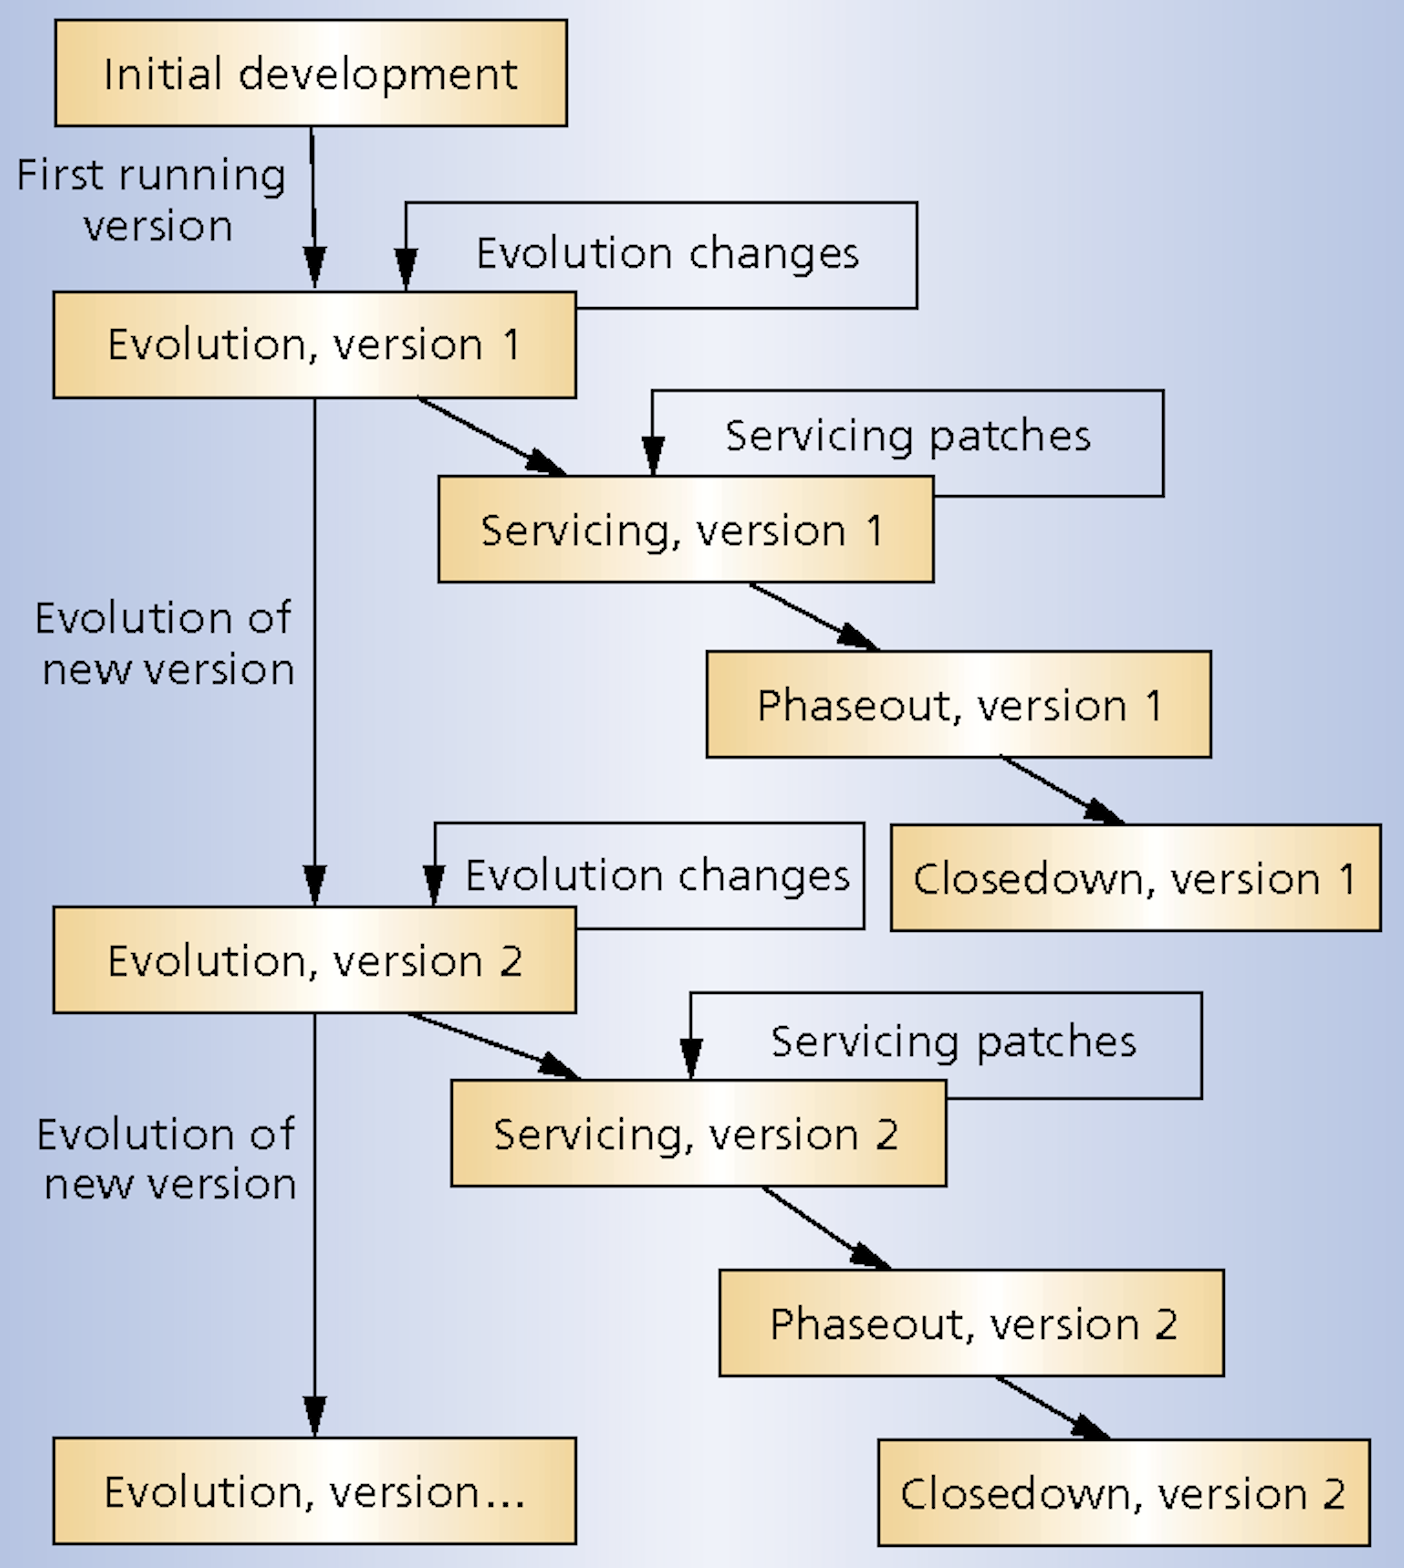
\includegraphics[scale=0.35]{JAI 2023/figures/staged-model-versions.png}
    \caption{\textit{O modelo de Rajlich com versões enfatiza a natureza evolutiva do desenvolvimento de software. Fonte:~\cite{rajlich:staged:2000}. }}
    \label{fig:staged:model}
\end{figure}

%Para o software de pesquisa, se existe um artigo de pesquisa que o utiliza, ...
%EXPLICAR que não há closedown... por causa da reprodutibilidade.
No contexto de desenvolvimento de \RS, 
deve-se considerar que ele se insere em um projeto de pesquisa que inclui \textit{dados e software}. 
No início do desenvolvimento do \RSw deve-se decidir
sobre a licença do software, onde o software será armazenado (por exemplo, GitHub, GitLab, etc.), tipo de sistema de versionamento e padrões de entrada e saída.
%
O lançamento de uma versão do \RSw e sua liberação para a sua comunidade podem ser motivados pela publicação de um artigo científico. O texto do artigo deve mencionar claramente a versão do \RSw utilizada. 

Também é essencial considerar a continuidade do \RSw ao longo do tempo e o suporte à  reprodutibilidade, especialmente quando o software for usado na pesquisa publicada em artigos científicos. 
Ao contrário de outros tipos de software, a etapa de Fechamento (\textit{Closedown}) não deveria ser considerada em \RSw para permitir a reprodutibilidade dos resultados divulgados nos artigos publicados.
Manter o \RSw vivo, disponível e acessível é fundamental para que outros cientistas possam reproduzir e verificar os resultados da pesquisa.

%\subsection{Dimensão Social}
\subsection{Pessoas} 

%A estrutura do grupo de pesquisa envolvido no desenvolvimento do software de pesquisa pode se refletir na estrutura do projeto ... 
%A pesquisa evolui, o grupo de pesquisa recebe novos membros, o software evolui, novo software pode ser criado que interfaceia com outros ...

%Holland: Many software maintenance problems are not technical but people problems\cite{versen_2020}
%We need to be able to organize the development team (group, community, etc.) in such a way that it embraces change and facilitates %maintenance and evolution, not only immediately after deployment of the software, but for the decades that follow.

Considerando que muitos problemas de manutenção de software não são problemas técnicos, mas problemas relacionados às pessoas~\cite{versen_2020}, percebemos que a dimensão social desempenha um papel importante na evolução do software, influenciando tanto o processo quanto o resultado final. 
As pessoas interessadas no desenvolvimento, utilização e manutenção de software têm um impacto significativo em sua evolução. A interação e colaboração entre os membros da equipe de desenvolvimento e os usuários contribuem com suas perspectivas e experiências, influenciando as decisões sobre novas funcionalidades, correções de \textit{bugs} e melhorias em geral. 
Além disso, as demandas e expectativas dos usuários, assim como  mudanças em suas necessidades e preferências podem exigir adaptações e atualizações do software para atender a essas demandas.

O caso específico da evolução de um \RSw  apresenta características distintas. 
O \RSw está inserido em um ecossistema científico, onde os pesquisadores buscam avançar o conhecimento em suas áreas. 
Nesse contexto, sua evolução está intimamente ligada à evolução da própria pesquisa e ao surgimento de novas abordagens e técnicas, exigindo atualizações e modificações no software. 
Além disso, a estrutura do grupo de pesquisa também influencia a evolução do software. À medida em que a pesquisa avança, novos membros ingressam no grupo, pesquisadores saem e a equipe se reconfigura. Tais mudanças na composição do grupo demandam mecanismos para transmitir o conhecimento legado e práticas estabelecidas.

%- Abrir para contribuição externa?
Tornar um \RSw disponível publicamente e aceitar contribuição de pessoas externas ao grupo de pesquisa pode resultar em uma comunidade maior de desenvolvedores envolvidos, facilitando o desenvolvimento mais rápido e eficiente, incluindo correções de \textit{bugs} e implementação de novos recursos de forma colaborativa. No entanto, a coordenação de um \RSw aberto pode exigir esforço adicional para estabelecer processos de governança e revisão de contribuições, para garantir que estas sejam de alta qualidade e estejam alinhadas com os objetivos do projeto. 
Além disso, a abertura precoce do \RSw pode expor pesquisas em andamento antes que estejam prontas para a publicação, o que pode comprometer a confidencialidade e ineditismo dos resultados.

%------------------------------------------
%\subsection{Práticas para o Desenvolvimento de Software} 

\subsection{Práticas} 

Há alguns anos a comunidade científica já reconhece ser essencial que cientistas, pesquisadores e estudantes sejam capazes de aprender e adotar um novo conjunto de habilidades e metodologias relacionadas a software~\cite{wssspe3}.
Alguns pesquisadores já abraçaram boas práticas de desenvolvimento de software e, em particular, uma classe especializada de desenvolvedores de software, chamados de \textit{Engenheiros de Software de Pesquisa} (\textit{Research Software Engineers}), está surgindo em ambientes acadêmicos como parte integrante de grupos de pesquisa bem-sucedidos~\cite{wssspe3}.
%
%\subsection{Ferramentas}
O uso consistente de boas práticas é apoiado por tecnologias e ferramentas conhecidas e tradicionalmente usadas por engenheiros de software.

%dentre elas, Git, Gitlab, Github, Docker.
%, bem como, ferramentas como R, Python, Latex, BibTex,  Workflow, Nextflow, etc etc.

\begin{comment}

\subsection{Engenheiros de Software de Pesquisa}

Engenheiros de Software de Pesquisa (\textit{Research Software Engineers}) ...
%
Engenharia de Software (engenheiro de software), Pesquisa (pesquisador).
%
O desenvolvimento de software de pesquisa requer indivíduos que combinem o melhor de ambas as funções (Figura~\ref{fig:rsengineering}).

\url{http://www.software.ac.uk/blog/2012-11-09-craftsperson-and-scholar}, \url{https://doi.org/10.5281/zenodo.7140726}. [KATZ]

\begin{figure}[htb]
    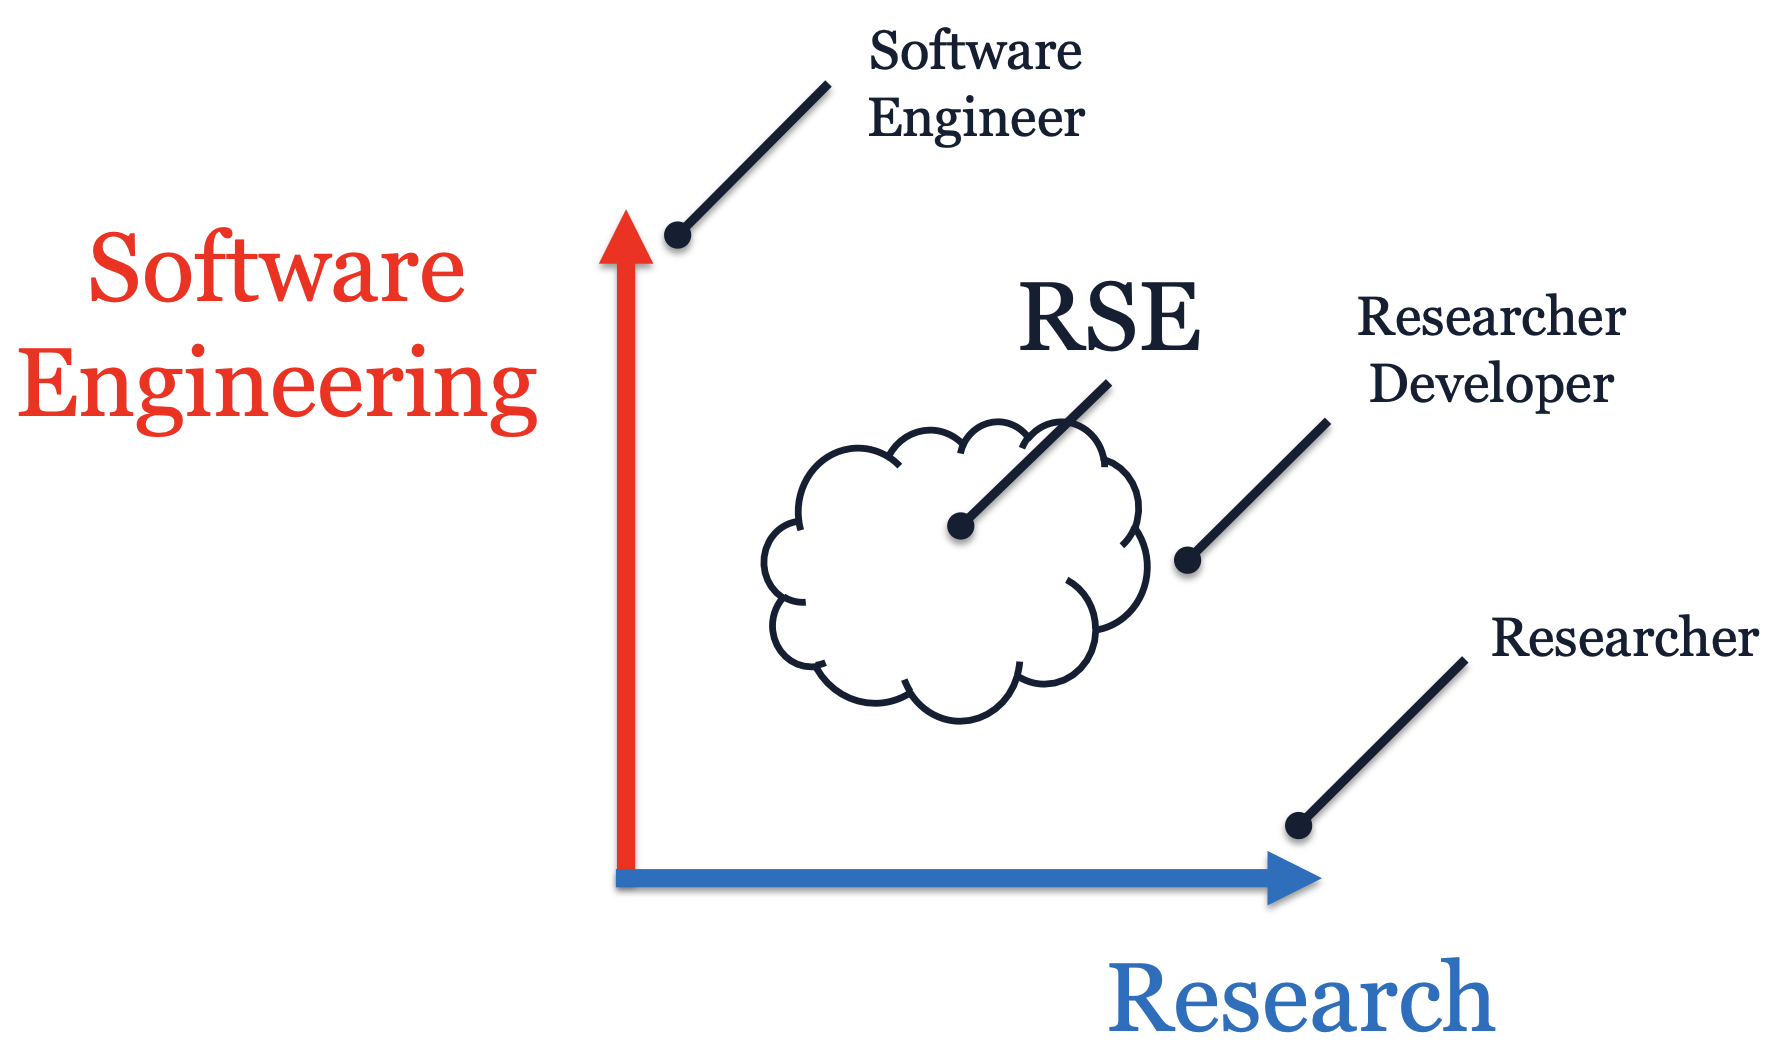
\includegraphics[scale=0.3]{JAI 2023/figures/research-software-engineering-katz.png}
    \caption{Caption [KATZ]}
    \label{fig:rsengineering}
\end{figure}

- Research Software Engineer (RSE)
+ Associations/societies
+ Career paths, structure

\end{comment}

% Alem da necessidade de politicas para melhorar a qualidade do codigo do software de pesquisa ha tambem a necessidade de politicas para incentivos a carreira do engenheiro de software de pesquisa e reconhecimento e visibilidade academica do seu trabalho.

%Desafios
%\begin{itemize}
%    \item Organizing and providing software training. 
     %Software-carpentry.org (http://software-carpentry.org/) provides the basic model to deliver that training.
%\end{itemize}


%--------------------------------%
%\subsection{Aspectos Avançados} %“I want to code better.” Provides more information on testing, continuous integration, release management, documentation, and other skills that help a programmer to produce higher-quality code.
%--------------------------------%

\section{Práticas para o Desenvolvimento de Software de Pesquisa Sustentável} \label{section:practices}

Projetos de software bem organizados adotam um modelo de desenvolvimento que resulta em código de alta qualidade que se adapta rapidamente a diferentes situações. Várias \textit{práticas} estabelecidas e usadas pelas comunidades de software livre são reconhecidas como contribuições importantes para a manutenção de \RSw de alta qualidade.
%
Nesta seção, apresentamos dezesseis boas práticas para uso em projetos de \RS, descritas e ilustradas no contexto de projetos hospedados no GitHub.
Parte do jargão técnico usado pelo GitHub não foi traduzido e alguns termos não foram definidos. Termos e suas definições podem ser encontrados no \textit{Glossário do GitHub}\footnote{\url{https://docs.github.com/en/get-started/quickstart/github-glossary}}.

\subsection{Práticas Básicas}

\subsection*{P1. Hospedagem do projeto} 

É recomendável hospedar e compartilhar o \RSw em um repositório público, exceto se houver questões de confidencialidade ou estratégicas relacionadas ao projeto de pesquisa (por exemplo, software implementa um algoritmo original, ainda não compartilhado amplamente com a comunidade científica). 
A hospedagem em repositório público pode ser estendida para todos os ativos da pesquisa, por exemplo, dados, fluxos de trabalho e relatórios.

A \textit{hospedagem pública do software} é fundamental para promover a reprodutibilidade, evitar a redundância (por exemplo, cópias do software em diversos repositórios locais), 
e estimular o compartilhamento entre pares da comunidade acadêmica.
%
A hospedagem pública do software e o acesso aos dados e fluxos de trabalho, permitem que os resultados da pesquisa possam ser verificados, replicados, e reproduzidos, fortalecendo a confiabilidade e a transparência dos estudos. 
%
Além disso, o \RSw hospedado torna-se localizável e acessível, facilitando seu uso ou reuso.
Se o código for aberto, outros pesquisadores podem se beneficiar dele, evitando o retrabalho e construindo sobre uma base já estabelecida. Isso promove a colaboração, a troca de conhecimentos e a aceleração do progresso científico.

\noindent \textbf{Exemplo.}
O \RSw \texttt{flosssearch} estava hospedado em uma pasta local no computador de um pesquisador. 
Por segurança, o pesquisador realizava backup manual periodicamente. 
Ao finalizar a implementação da primeira funcionalidade do software, o pesquisador decidiu que o projeto precisava ser hospedado adequadamente e compartilhado com outros membros do grupo de pesquisa.
%Uma organização foi criada no GitHub e o
O software \texttt{flosssearch} foi colocado em um repositório público no GitHub, uma plataforma baseada na web onde os usuários podem hospedar repositórios, compartilhar e promover a colaboração em projetos de software.
%
O repositório foi compartilhado com dois pesquisadores do grupo.
% Mensagem de \textit{commit}: \textit{v 0.0.1 - Versionando}.

Ao ser hospedado no GitHub, o software recebeu uma URL, um nome oficial e a sua identidade foi definida, de forma clara e única. 
O nome oficial público atribuído ao \RSw é \texttt{flosssearch}.
Além disso, o software \texttt{flosssearch} passou a contar com um serviço de backup, considerando que os arquivos do projeto e todo o seu histórico são armazenados no servidor remoto e nos repositórios locais dos pesquisadores.

\subsection*{P2. Controle de versão} 

Controle de versão é a prática de rastrear e gerenciar alterações no código de um software. 
Os sistemas de controle de versão são ferramentas que
permitem que várias versões do mesmo \RSw sejam mantidas e, possivelmente, referenciadas por experimentos de pesquisa e artigos científicos. 
Um sistema de controle de versão também permite o acompanhamento das atividades realizadas, fornece um registro das alterações e permite que desenvolvedores e usuários do \RSw acompanhem o seu desenvolvimento e evolução, tornando a pesquisa mais aberta
e reprodutível. 
Ao usar o controle de versão, o pesquisador nunca perde as versões anteriores do \RS, e erros podem ser revertidos.
Adicionalmente, o versionamento do software também promove a colaboração entre pesquisadores.

%It is highly recommended to start using version control on day one of the project.

\noindent \textbf{Exemplo.}
A plataforma GitHub utiliza o Git\footnote{\url{https://git-scm.com}}, um sistema de controle de versão distribuído gratuito e de código aberto. 
Ao ser colocado no GitHub, com um nome e repositório associado, 
o \RSw \texttt{flosssearch} recebeu suporte para controle de versão distribuído. 
%... versão  \textit{v 0.0.1 - Versionando projeto} ... 4 anos atrás.

\subsection*{P3. Licenças de Software} 
% Nesta seção apresentaremos aspectos de Licenças de Software relevantes para o Software de Pesquisa e para alavancar a Ciência Aberta. 

%Alguns dos tópicos: \textit{Open Source Software}, \textit{Open Source Initiative}\footnote{\url{https://opensource.org/licenses}}, licenças populares e amplamente utilizadas ou com comunidades fortes, tais como a GNU General Public License (GPL) ou a Mozilla Public License 2.0.

% Olhar no GitHub o projeto ChooseaLicense

A licença de software escolhida é essencial para o \RSw disponível publicamente. O financiamento do projeto pode terminar após um certo período, e os mantenedores podem terminar suas pesquisas ou mudar de área de interesse. Assim, para garantir a disponibilidade contínua do projeto, os desenvolvedores precisam chegar a um acordo formal, ou seja, uma licença de software em que os termos de uso sejam explícitos.

Recomenda-se que projetos de \RSw de código aberto sejam lançados sob uma licença compatível com a GNU General Public License - GPL\footnote{\url{https://www.gnu.org/licenses/gpl-3.0.html}},
a licença OSS mais popular e amplamente utilizada.
Outras licenças de software de código aberto e suas descrições podem ser encontradas no site da Open Source Initiative (OSI)\footnote{\url{https://opensource.org/licenses/}}.

O GitHub permite que o usuário escolha uma licença de software para o seu repositório e cria automaticamente o arquivo \textit{LICENSE} com uma cópia da licença escolhida.
Entretanto, apenas colocar uma cópia da licença em um arquivo em seu repositório não declara explicitamente que o código no  repositório pode ser usado sob tal licença. 
Sem uma declaração explícita, não fica claro se as permissões da licença se aplicam a qualquer arquivo fonte no repositório.

A Figura~\ref{fig:warranty} mostra um aviso que o desenvolvedor deve incluir no início de cada arquivo fonte para declarar a licença e a exclusão da garantia. Cada arquivo deve ter pelo menos a linha ``copyright'' e indicação sobre local onde o aviso completo pode ser encontrado.
%
A falta de uma licença claramente definida pode gerar incerteza legal e dificultar a contribuição e o compartilhamento do software, já que os colaboradores podem ficar inseguros sobre seus direitos e obrigações, o que pode limitar a adoção e colaboração.

\renewenvironment{quote}
  {\small\list{}{\rightmargin=1cm \leftmargin=1cm}%
   \item\relax}
  {\endlist}
\begin{figure}[htb]
    \centering
\begin{quote}
\textit{<one line to give the program's name and a brief idea of what it does.>}
    
Copyright (C) \textit{<year>}  \textit{<name of author>}

This program is free software: you can redistribute it and/or modify it under the terms of the GNU General Public License as published by the Free Software Foundation, either version 3 of the License, or (at your option) any later version.

This program is distributed in the hope that it will be useful, but WITHOUT ANY WARRANTY; without even the implied warranty of MERCHANTABILITY or FITNESS FOR A PARTICULAR PURPOSE. See the
GNU General Public License for more details.
You should have received a copy of the GNU General Public License along with this program.  If not, see <https://www.gnu.org/licenses/>.
\end{quote}
\caption{Declaração explícita sobre uso de licença GPL e exclusão da garantia.} \label{fig:warranty}
\end{figure}

\noindent\textbf{Exemplo.}
Ao ser colocado em um repositório público no GitHub, 
o \RSw \texttt{flosssearch} tornou-se visível, acessível e utilizável por terceiros, sendo necessária a escolha de uma licença de código aberto. Os pesquisadores escolheram a licença GNU GPL 3.0. 
Além do arquivo LICENSE, os arquivos com código-fonte do projeto possuem uma breve descrição sobre o seu propósito, a linha ``copyright'' e indicação sobre a licença de software escolhida e onde o texto completo pode ser encontrado (Figura~\ref{fig:license:moara}).

%Apesar da linguagem PHP possuir um framework para automação de testes, o \textit{PHPUnit}, o software \texttt{flosssearch} não possui testes automatizados. 
%A falta de testes pode dissuadir desenvolvedores de consertar, estender ou melhorar o \RS, e outros pesquisadores de usá-lo. 

\renewenvironment{quote}
  {\small\list{}{\rightmargin=1cm \leftmargin=1cm}%
   \item\relax}
  {\endlist}
\begin{figure}[htb]
\centering
\begin{quote}
\texttt{flossearch} is a web application designed to support instructors and students in selecting OSS projects for Software Engineering Education.

Copyright (C) \textit{2021}  \textit{Moara Brito}

This program is free software: you can redistribute it and/or modify it under the terms of the GNU General Public License 3.0 <https://www.gnu.org/licenses/>.
\end{quote}
\caption{Declaração sobre uso de licença GPL para inclusão nos arquivos do \texttt{flosssearch}.} \label{fig:license:moara}
\end{figure}

% O arquivo README.md ...

\subsection*{P4. Registro de Software}

O \RSw deve ser publicado formalmente para satisfazer os princípios FAIR, promover a sustentabilidade de software e permitir a citação de software. Os repositórios de publicação dão suporte ao registro do software e fornecem versões de software publicadas com identificadores únicos e persistentes, como um DOI.

Há várias formas de associar um DOI a um repositório GitHub. 
Zenodo\footnote{\url{https://zenodo.org}} e Figshare\footnote{\url{https://figshare.com}} 
podem ser utilizados para fazer o registro do DOI e arquivar versões especificas do software. 
%
Há também o projeto {\em The Research Software Directory}\footnote{\url{https://research-software-directory.org}} desenhado para centralizar metadados de software de pesquisa e mostrar os seus impactos na pesquisa e na sociedade, estimulando o reuso de software e encorajando a citação de maneira apropriada para garantir que pesquisadores e engenheiros de \RSw  recebam créditos por seus trabalhos. 

\noindent \textbf{Exemplo.}
O \RSw \texttt{Parcels}\footnote{\url{https://github.com/OceanParcels/parcels}} (\textbf{P}robably \textbf{A} \textbf{R}eally \textbf{C}omputationally \textbf{E}fficient \textbf{L}agrangian \textbf{S}imulator) é um conjunto de classes e métodos em Python para criar simulações de rastreamento de partículas, como plâncton, plástico e peixes. 
O \texttt{Parcels} está registrado no Research Software Directory\footnote{\url{https://research-software-directory.org/software/parcels}}.


%O Zenodo se integra ao GitHub para arquivar o software e fornecer um DOI quando os desenvolvedores fizerem um lançamento formal no GitHub.

%\noindent \textbf{\texttt{seed.select}}.

% Movi pra parte de Avaliação
%\noindent \textbf{\texttt{Software MoSyn}}.
%O repositório não menciona se há um DOI associado a ele e não encontramos referência ao software no Zenodo.


%---------------------------------------------%
\subsection{Organização do Projeto}

O suporte à reprodutibilidade na pesquisa que utiliza um \RSw requer que seus artefatos estejam bem organizados em um repositório aberto. 

\begin{figure}[htb]
    \centering
    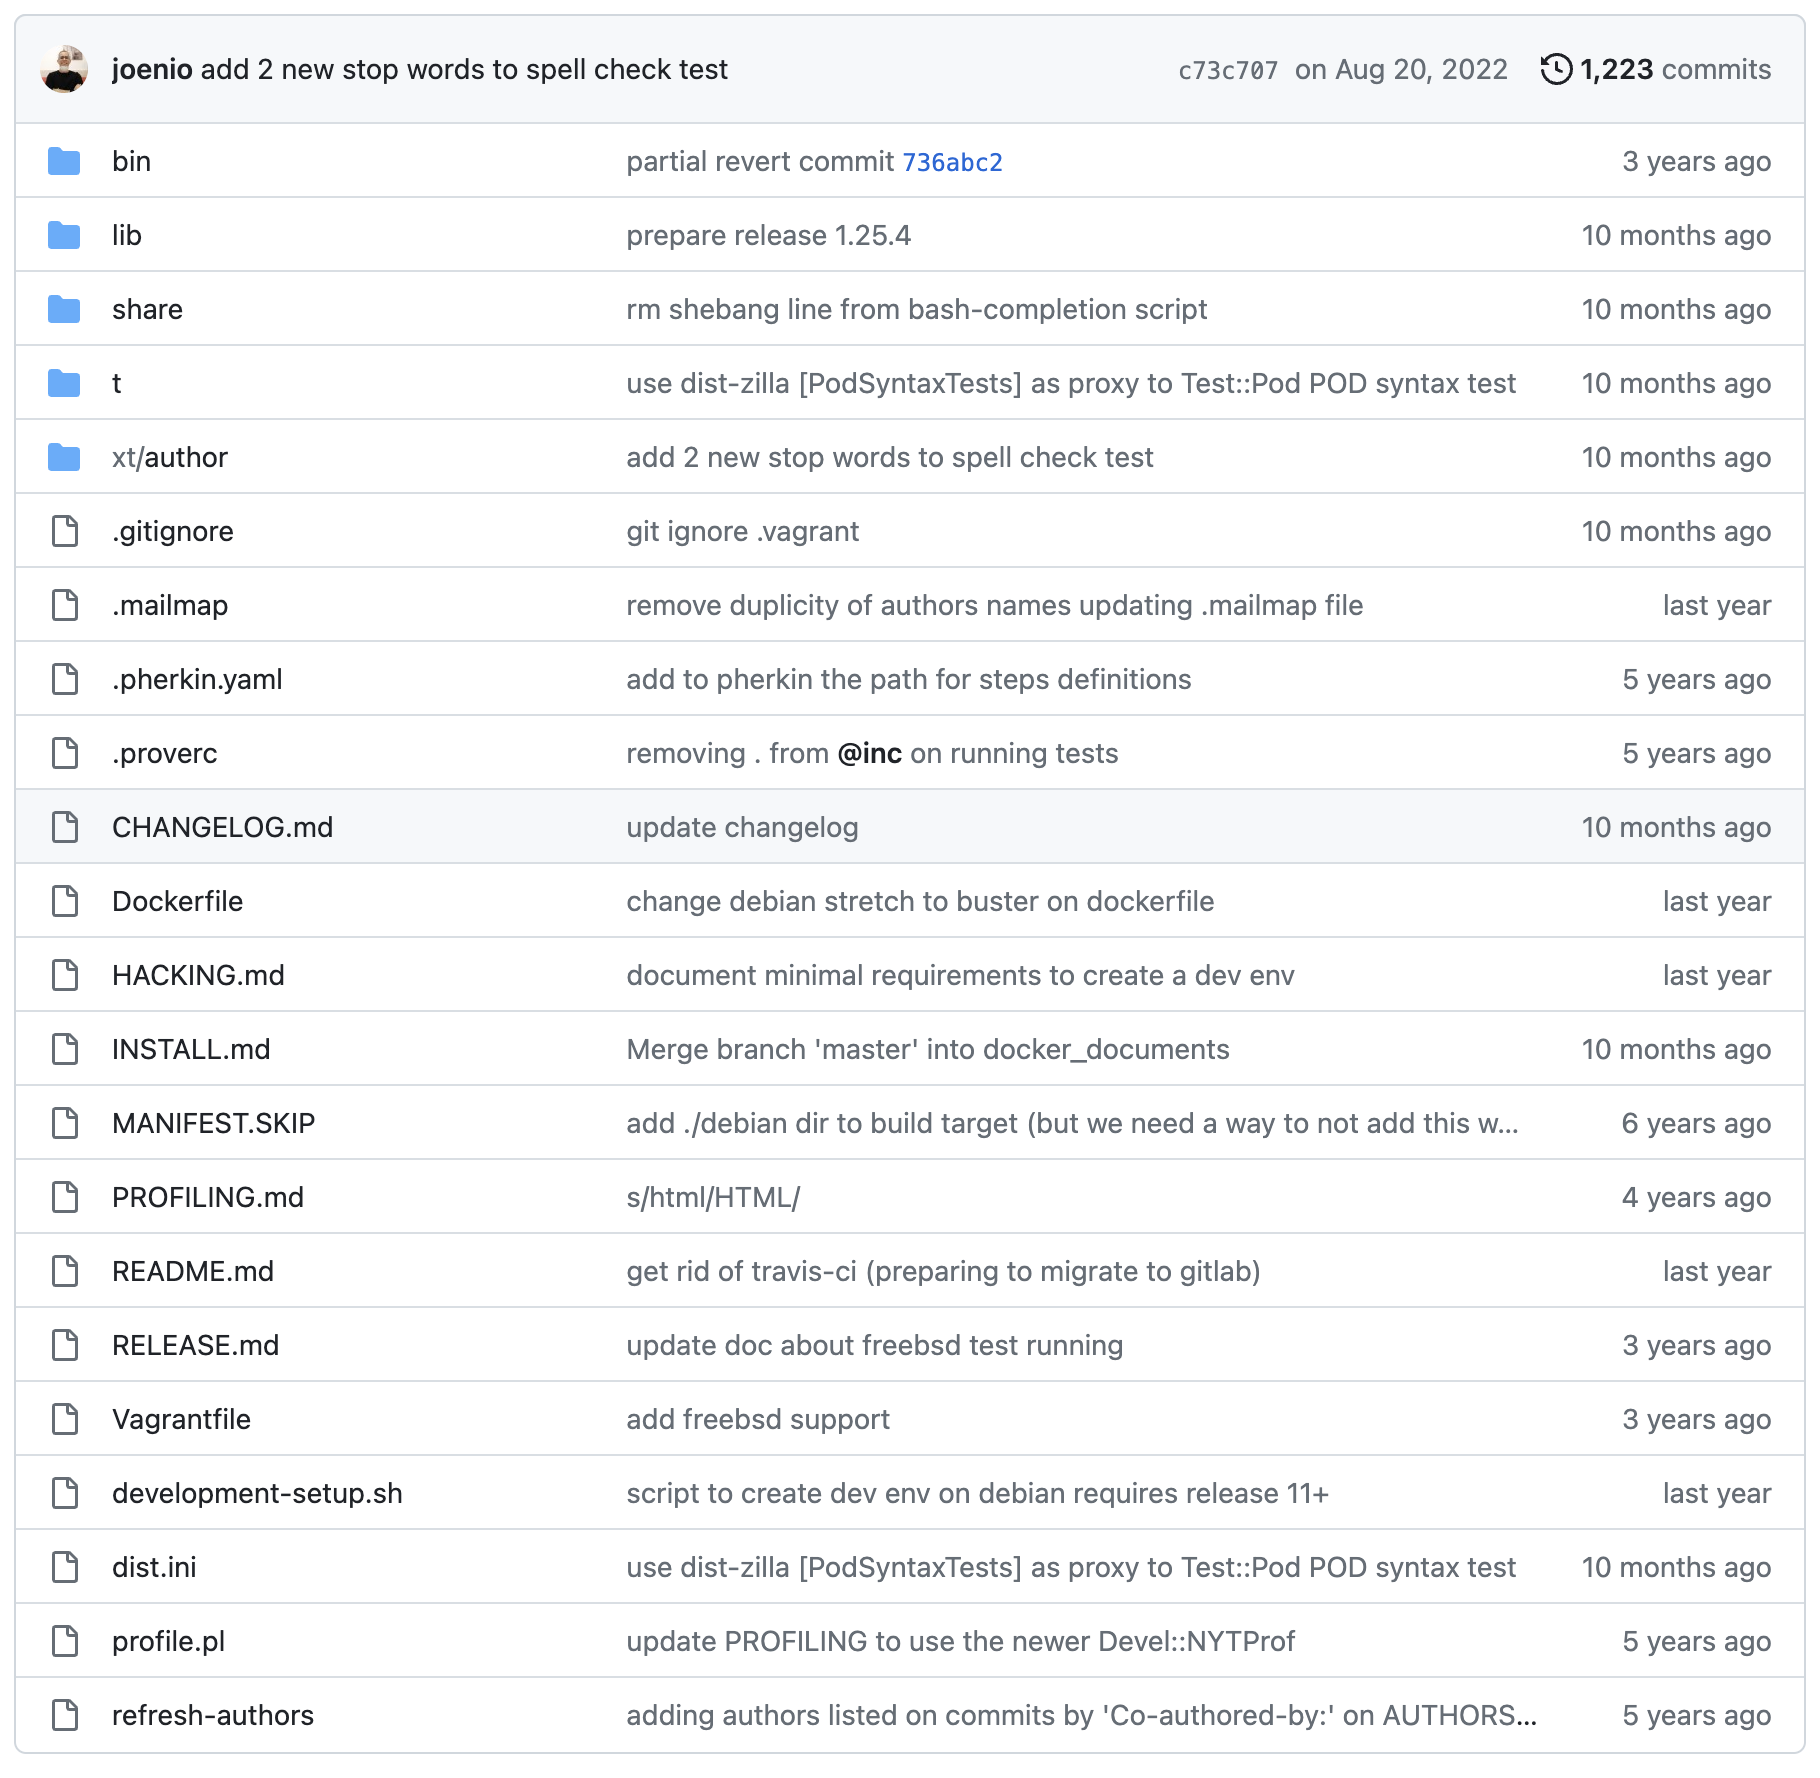
\includegraphics[scale=0.45]{JAI 2023/figures/analizo-estrutura.png}
    \caption{Estrutura de arquivos da ferramenta \texttt{Analizo}.}
    \label{fig:estrutura:analizo}
\end{figure}

\subsection*{P5. Estrutura} 

É importante ter uma estrutura de arquivos que comunica a finalidade dos elementos dentro de um \RS, separando os interesses em uma hierarquia de pastas e usando nomes auto-explicativos, facilitando a compreensão de todos que tenham interesse revisitar, revisar e desenvolver o software.

\noindent\textbf{Exemplo.} A Figura~\ref{fig:estrutura:analizo} apresenta a estrutura de arquivos da ferramenta de análise estática \texttt{Analizo}\footnote{\url{https://github.com/analizo/analizo}}\cite{analizo2010}, desenvolvida como \RSw no contexto de uma pesquisa de doutorado. Pode-se observar que há pastas e arquivos com nomes auto-explicativos, por exemplo, \textit{bin}, \textit{lib} e \textit{share}, INSTALL.md, README.md.

\subsection*{P6. Padronização} 
% Use standards

%O uso de formatos de dados e interfaces padronizados facilita a integração com outros sistemas e desencoraja a dependência de fornecedores específicos. 

A padronização e o uso de protocolos de comunicação entre sistemas tem uma grande importância no software de pesquisa. A partir da adoção de padrões e protocolos bem definidos, os diferentes sistemas podem interagir de forma consistente, facilitando a integração e desencoraja a dependência de fornecedores específicos. Além disso, a padronização simplifica a interoperabilidade e a reutilização de componentes de software, permitindo que os pesquisadores desenvolvam seus trabalhos sobre trabalhos existentes e tornem mais rápido o desenvolvimento de novas soluções.

\noindent\textbf{Exemplo.} O software \texttt{MoSyn} é um \RSw que se preocupa com padronização pois depende de um software proprietário, o  MATLAB\footnote{\url{https://www.mathworks.com/products/matlab.html}}. A Seção~\ref{section:casesstudy:mosyn} apresenta uma avaliação do \texttt{MoSyn} com base nas práticas para o desenvolvimento adotadas.

%---- Qualidade -----%
% Geral: Higher quality software has fewer defects, better security, and better performance, which leads to happier users who can work more effectively.

\subsection*{P7. Documentação} 

A documentação frequente e contínua é uma prática recomendada para manter guias do usuário, manuais e outros documentos relevantes atualizados em relação à versão mais recente do software, facilitando o entendimento e colaboração.
Para o \RS, a documentação é um pré-requisito fundamental para reuso e reprodução de estudos~\cite{chue_hong_fair_2022}.
%
\cite{herman:2022} analisaram o estado-da-prática sobre documentação de \RS. Eles reportaram que, ainda que alguns guias com boas práticas científicas valorizem e recomendem a prática de documentar explicitamente~\cite{deutsche_forschungsgemeinschaft_2022_6472827},  
a documentação do \RSw ainda é considerada inadequada~\cite{wilson2017good, chue_hong_fair_2022}.

%- Como manter a documentação atualizada?

%Developers usually change code, correcting bugs, adding new functionalities but not do any modification in documentation, this turn it outdated. However the documentation is useful only if it's up to date. 
%
%Before you submit your change, write the documentation related to it.
%Core developers should require this from the contributors.

A documentação de um projeto só é útil se está atualizada. Por isso, uma questão importante em um projeto de software é a sincronização entre o desenvolvimento do software e a documentação dele, garantindo que a documentação representa a versão mais atualizada do software. 
Para conseguir essa sincronização é essencial integrar o processo de atualização da documentação no ciclo de desenvolvimento do software. Além disso, é possível automatizar a geração de documentação a partir de comentários no código-fonte, reduzindo o esforço necessário para manter a documentação atualizada.

Em geral, geradores de documentação são usado para interfaces de programação de aplicativos (APIs), destinadas a um público de desenvolvedores. 
\textit{Doxygen}\footnote{\url{https://www.doxygen.nl}} é uma ferramenta que extrai documentação a partir do código-fonte e de outros arquivos e gera uma versão em formato estruturado, como HTML, PDF ou LaTeX. 
%
Doxygen é a ferramenta padrão de fato para gerar documentação para C++, mas também suporta outras linguagens de programação populares como C, Objective-C, C\#, PHP, Java e Python.

Uma documentação precisa ser clara e considerar os diferentes interessados no \RS. A documentação precisa atender às necessidades específicas de cada grupo, usando linguagem e terminologia que ajudem cada público a compreender e utilizar as informações de maneira eficaz.

%- Como escrever documentação clara e útil para desenvolvedores?
%Para escrever documentação clara e útil para desenvolvedores
A \textit{documentação para desenvolvedores} deve abordar aspectos técnicos, como arquitetura, APIs, dependências e configurações, incluindo descrições detalhadas de como utilizar as funcionalidades do software. É importante que sejam fornecidas orientações passo-a-passo sobre instalação, configuração, execução e dependências necessárias para o ambiente de desenvolvimento do software. 
Para facilitar a contribuição, é essencial descrever conceitos fundamentais, padrões de codificação e boas práticas de desenvolvimento.
Testes de software também oferecem uma forma de documentar a funcionalidade do software por meio da
qual desenvolvedores podem ter uma visão mais detalhada sobre o funcionamento interno do software e integração com outros sistemas.

%- Como escrever documentação útil para não desenvolvedores, outros pesquisadores?
Na \textit{documentação para pesquisadores} que não são desenvolvedores, deve-se utilizar uma linguagem acessível, evitando jargões técnicos e explicando conceitos de forma simples e compreensível. 
A descrição da utilização deve destacar as  funcionalidades e benefícios do software. 
Para facilitar o uso, podem ser apresentados exemplos práticos de como o \RSw pode ser aplicado em diferentes cenários e incluir uma seção de perguntas frequentes para responder às dúvidas mais comuns dos usuários. Dessa forma, a documentação para os pesquisadores que não são desenvolvedores pode ajudá-los a entender como utilizar o software de forma prática para atingir seus objetivos de pesquisa, sem detalhes técnicos desnecessários.

Para todos os tipos de usuários,
recomenda-se que, ao publicar o \RS, o desenvolvedor  disponibilize uma página de boas-vindas e descrição do software. Isso pode ser feito facilmente com um arquivo \textit{README} colocado no diretório raiz do projeto.
Uma boa descrição sintetiza as funcionalidades do \RSw e permite que outros pesquisadores possam decidir se querem usá-lo ou não. O desenvolvedor também deve incluir informações de contato e canais de suporte, como e-mail, fórum de discussão e indicar ferramentas  que podem ser usadas para que os usuários solicitem ajuda adicional.

\begin{figure}[tb]
    \centering
    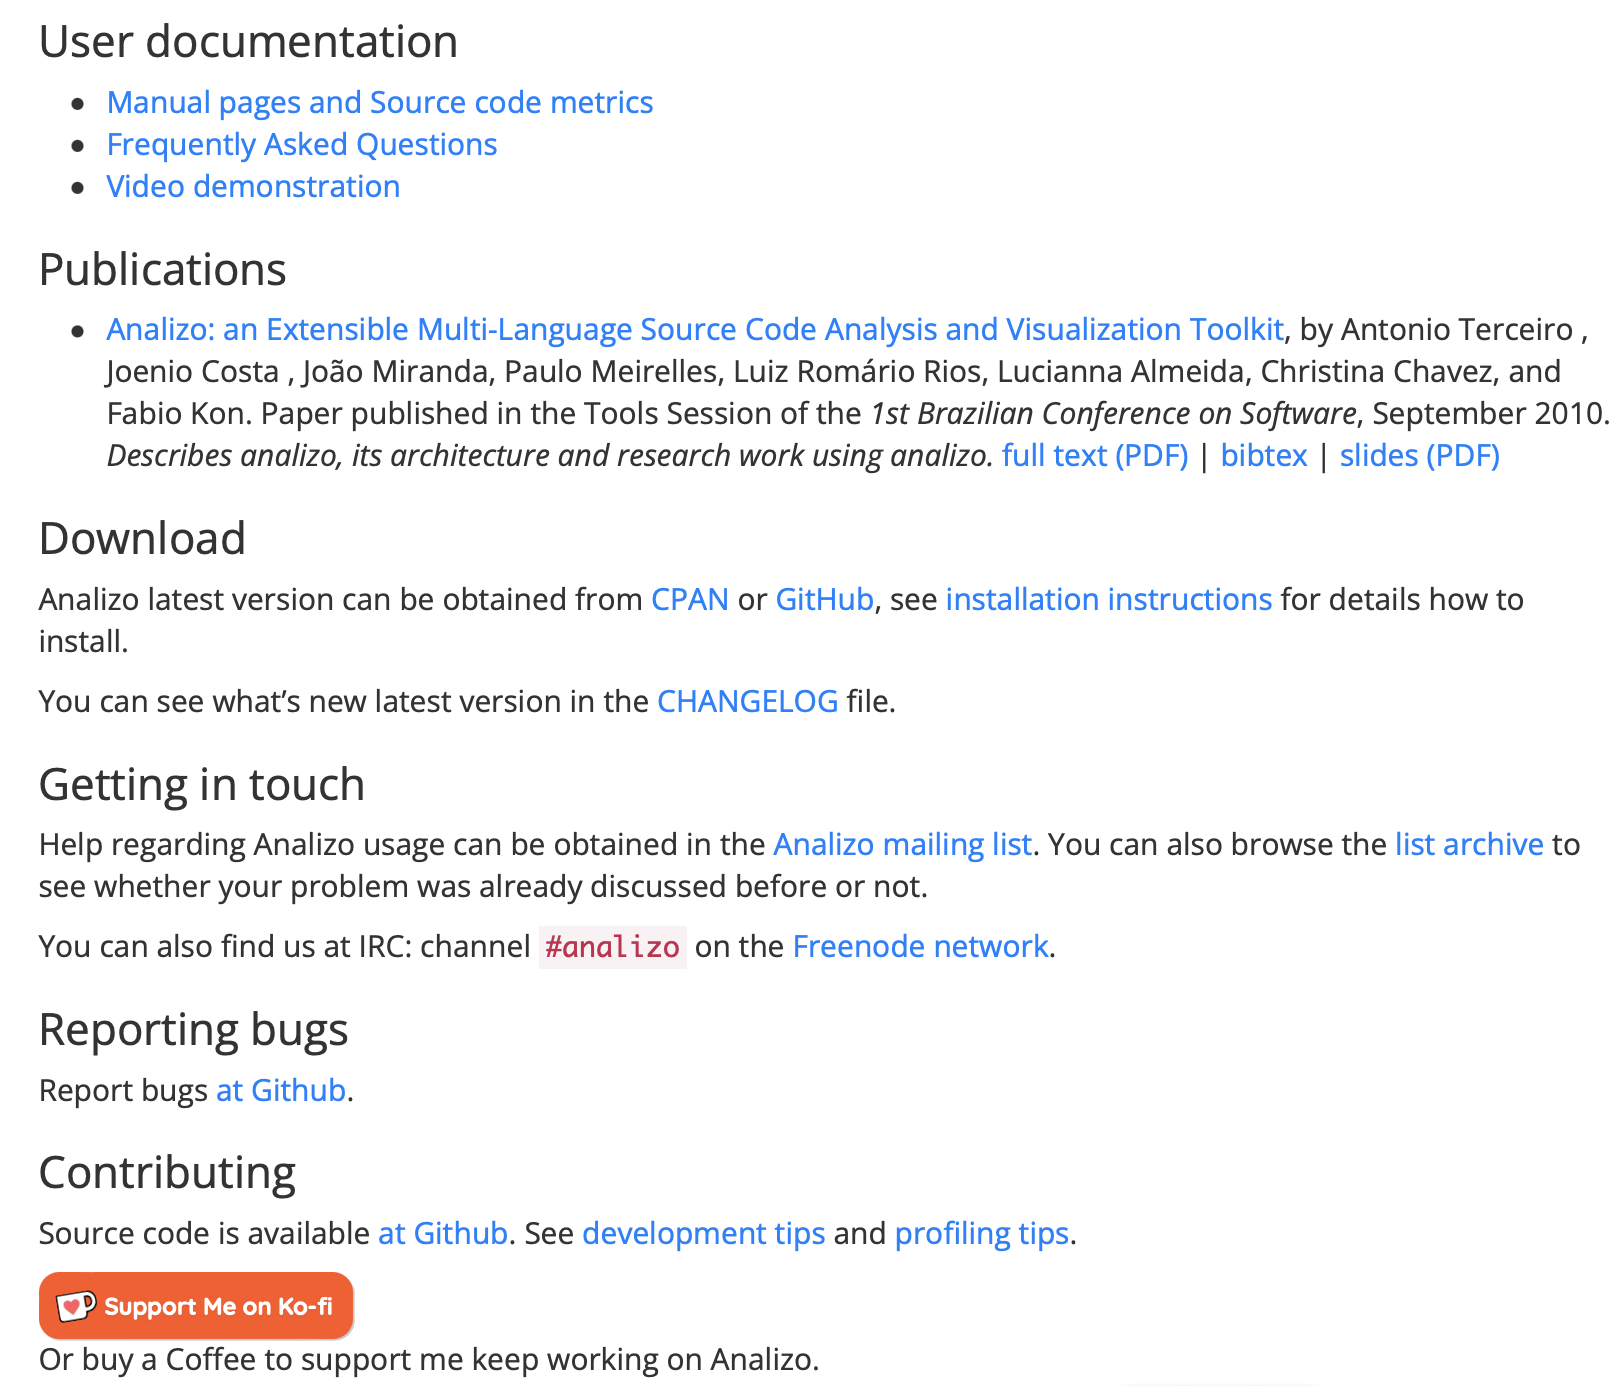
\includegraphics[scale=0.5]{JAI 2023/figures/analizo-website.png}
    \caption{Documentação para usuários da ferramenta \texttt{Analizo}}
    \label{fig:documentacao:analizo}
\end{figure}

%\noindent \textbf{\# \texttt{flossSearch}}.
\noindent \textbf{Exemplo}.
O software \texttt{flosssearch} disponibiliza para os usuários informações sobre funcionalidades, tecnologias e licença utilizada, em um arquivo README, sob controle de versão, que pode ser atualizado regularmente. Porém, não há informações de contato ou sobre canais de comunicação.
A Figura~\ref{fig:documentacao:analizo} mostra uma parte da excelente documentação para usuários disponibilizada no website da ferramenta \texttt{Analizo}\footnote{\url{https://www.analizo.org}}.

%No software \texttt{flosssearch} não há documentação para desenvolvedores com descrição de padrões, ferramentas, fluxos de trabalho, ou testes. 

\subsection{Qualidade}

O processo de garantia da qualidade do \RSw é tão necessário quanto o código que foi escrito.
\textit{Confiabilidade} é um dos atributos de qualidade do software, em geral definido como a probabilidade do mesmo funcionar sem a ocorrência de falhas em um período específico.
Testes e revisão de código são duas técnicas populares que podem ser usadas no desenvolvimento de \RSw confiável.

%----------------------------------%
%Qual a importância dos testes automatizados para o software de pesquisa? 
%Para o software de pesquisa testes podem aumentar a confiabilidade que os resultados produzidos pelo software são mais confiáveis.
%Tipos de testes. testes de unidade e de integração.
%Ferramentas para automação de testes
%------------------------------------%

\subsection*{P8. Teste de software} 

\textit{Teste de software} é a atividade de executar um produto de software para verificar se ele está em conformidade com suas especificações.
Testes fornecem evidências sobre a confiabilidade do software, além de promover agilidade e, possivelmente, redução nos custos de desenvolvimento, depuração e manutenção do software~\cite{maldonado:book}.  

O uso contínuo desta prática protege o \RSw em relação à introdução de \textit{bugs} em correções ou modificações futuras.
%Testes também podem servir para documentar interfaces externas e de funções internas do software.
\textit{Testes de unidade} são usados para testar métodos, funções, \textit{scripts} e outros tipos de unidades de programa, concentrando-se nas saídas geradas em resposta às entradas e às condições de execução~\cite{maldonado:book}. Em geral, os \textit{testes funcionais} tratam o sistema como uma ``caixa preta'', pelo fato de não haver acesso aos detalhes de código para a criação dos casos de teste.

Há diversos \textit{frameworks} disponíveis para criação e \textit{automação de testes} funcionais e de unidade para linguagens de programação popularmente usadas no desenvolvimento de \RS, por exemplo, \textit{JUnit} (http://junit.org/) para Java, \textit{CUnit} (http://cunit.sourceforge.net/) para C, 
\textit{py.test} (http://pytest.org/) para Python e \textit{PHPUnit} (https://phpunit.de) para PHP.

\noindent\textbf{Exemplo.} A ferramenta de análise estática \texttt{Analizo} possui um conjunto de testes automatizados. 
%
A Figura~\ref{fig:testes:analizo} mostra informações sobre como executar seus testes.

%Mostrar um projeto de software de pesquisa que tem testes.
\begin{figure}[tb]
    \centering
    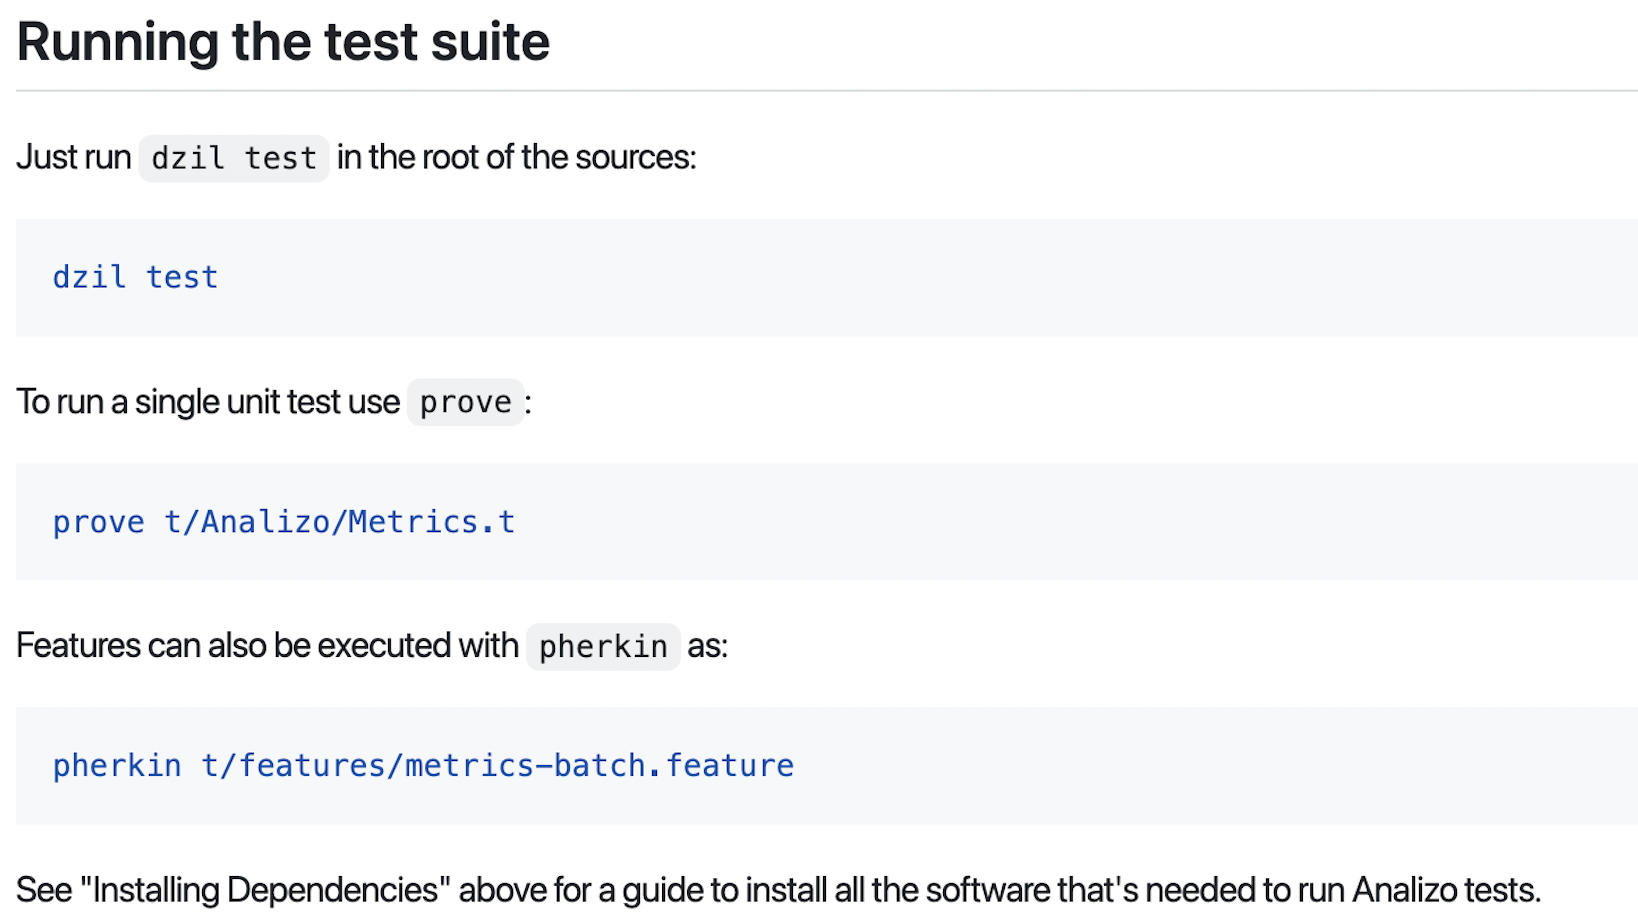
\includegraphics[scale=0.5]{JAI 2023/figures/analizo-tests.png}
    \caption{Trecho da documentação no GitHub mostrando como executar os testes da ferramenta \texttt{Analizo}.}
    \label{fig:testes:analizo}
\end{figure}

Apesar da linguagem PHP possuir um framework para automação de testes, o \textit{PHPUnit}, o software \texttt{flosssearch} não possui testes automatizados. 
A falta de testes pode desestimular os desenvolvedores para consertar, estender ou melhorar o \RS, e desencorajar outros pesquisadores a usá-lo. 

\subsubsection*{P9. Revisão de código} 
% Code reviews are an effective method for improving software quality. 

Revisão de código, ou revisão por pares, é uma prática consolidada para a melhoria da qualidade do software.
A colaboração entre pares durante a revisão é facilitada por meio do acesso compartilhado ao código-fonte e vários canais de comunicação. 
Outros desenvolvedores podem perceber problemas na qualidade do  código do \RSw que testes automatizados podem não detectar. 
Os revisores podem identificar alguns tipos de \textit{bugs}, problemas lógicos, falta de padronização e de conformidade com as práticas e diretrizes do projeto.

No contexto do \RS, a revisão de código pode, além de promover a melhoria da qualidade do software, ser aplicada a outros ativos da pesquisa. 
%
A revisão de código também permite que outros desenvolvedores e pesquisadores avaliem se os métodos aplicados e implementados no \RSw estão em conformidade com as teorias subjacentes da pesquisa. A falta de conformidade entre teoria e implementação em um \RSw  pode levar a conclusões errôneas em todo um estudo e seus resultados.

% Boas práticas na revisão de código.
% Ferramentas.

\noindent \textbf{Exemplo.}
Ao ser colocado em um repositório público, o software 
\texttt{flosssearch} foi compartilhado e pôde ser revisado por outros pesquisadores.
O texto de apresentação mostrado na tela principal do \texttt{flosssearch} em execução, foi revisado por outro pesquisador do grupo e algumas inconsistências foram reportadas e corrigidas.

% Movi pra parte de Avaliação
%\noindent \textbf{\texttt{Software Mosyn}}.
%Por estar publicado no GitHub, é possível fazer \textit{pull requests} e a realização de revisão de código. Até o dia da avaliação, todos os \textit{pull requests} listados no repositórios foram aprovados pelo próprio autor, sugerindo que não houve revisão de código por outra pessoa

\subsection{Gerência}

As práticas de gerência apresentadas estão relacionadas aos processos e ferramentas usados para acompanhar e aumentar a eficiência de tarefas de desenvolvimento do \RS. 

\begin{figure}[tbp]
    \centering
    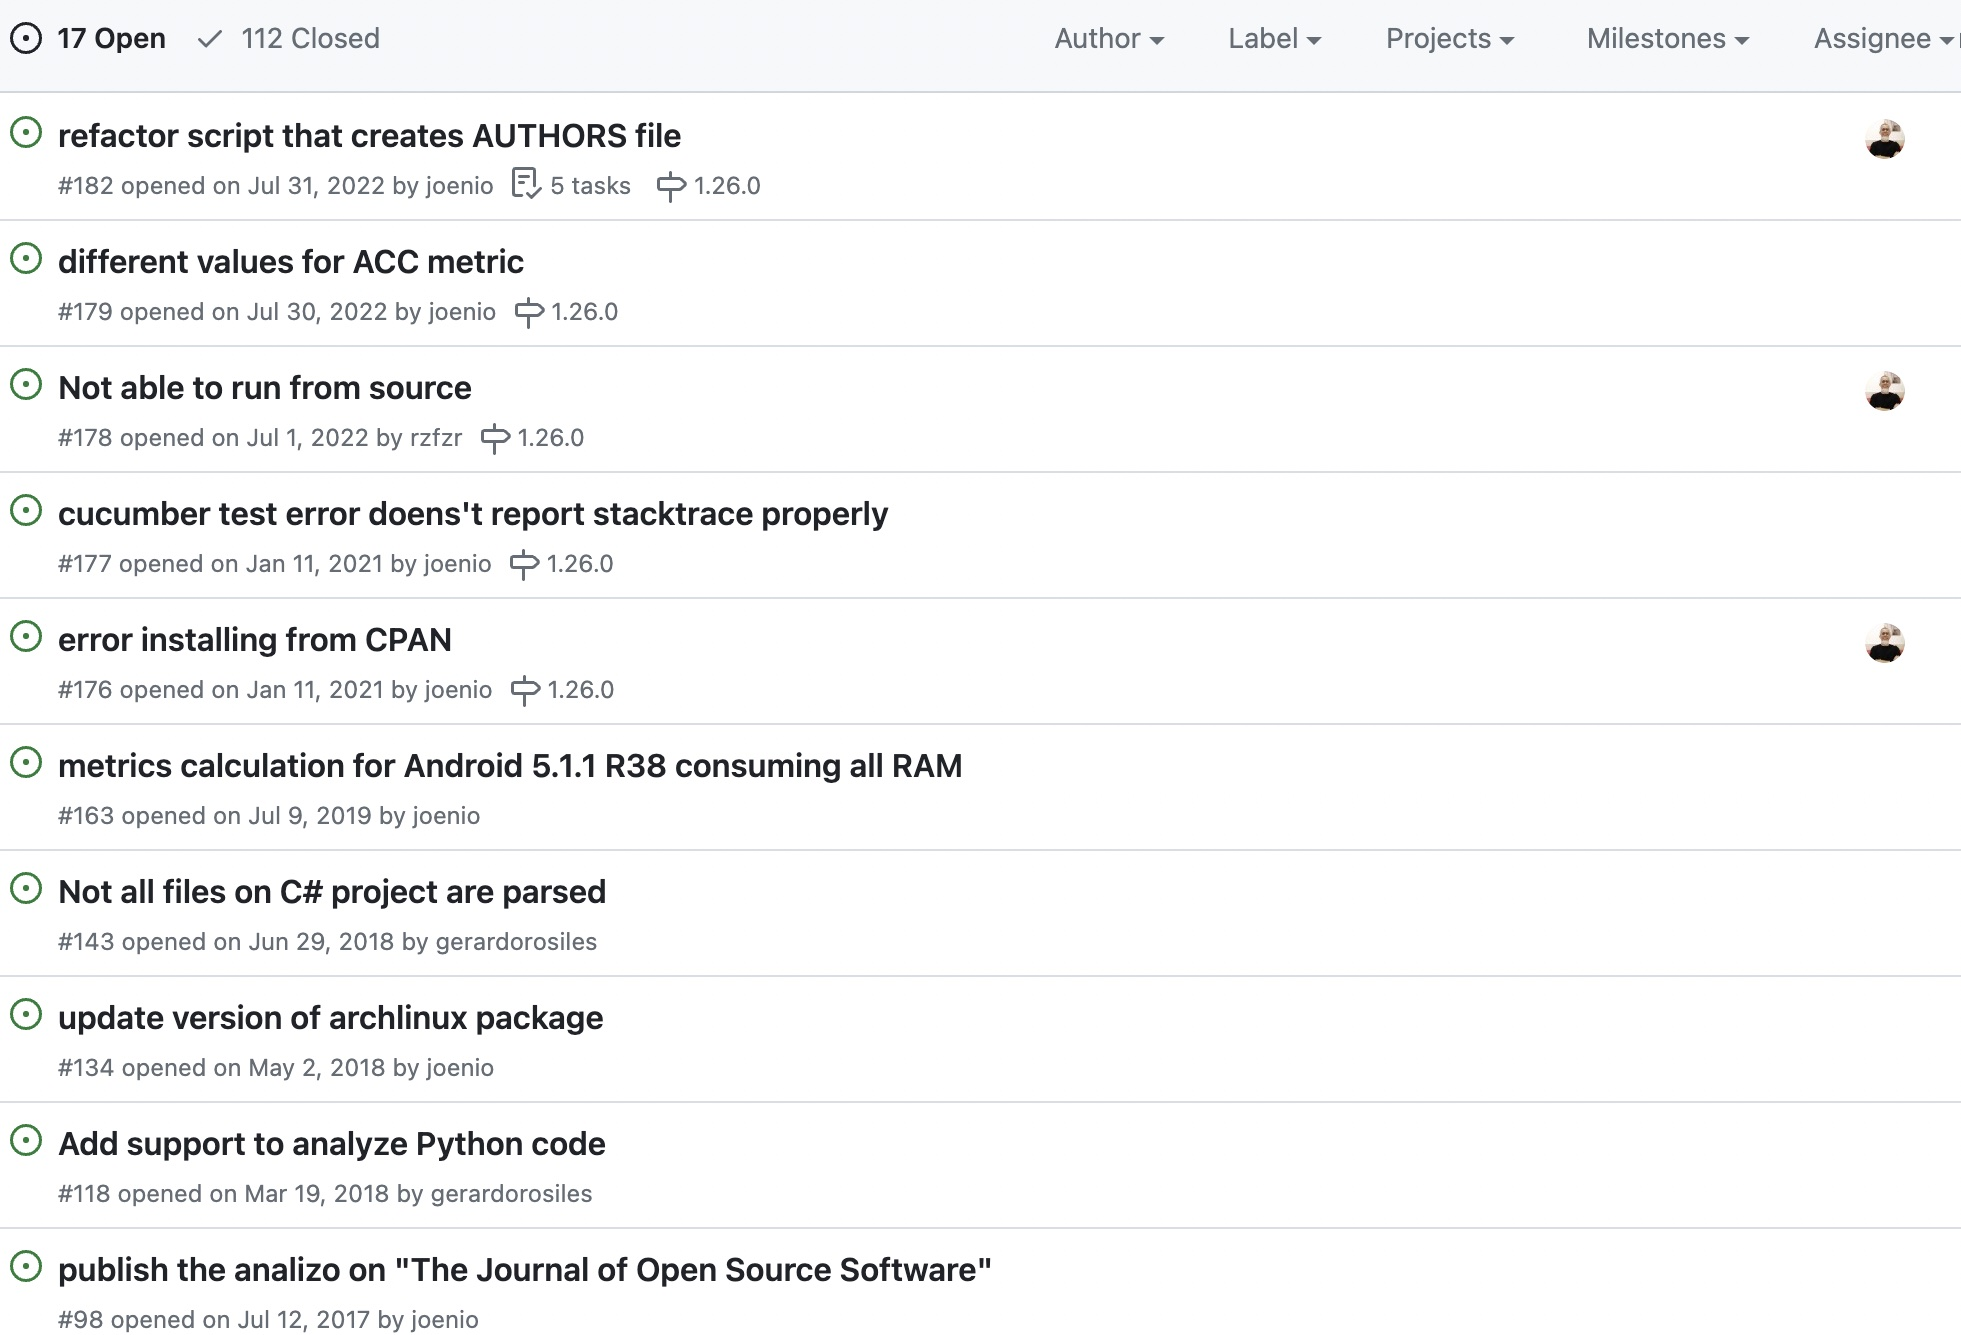
\includegraphics[scale=0.215]{JAI 2023/figures/analizo-issues.jpg}
    \caption{\textit{Issue tracker} da ferramenta \texttt{Analizo} no GitHub.}
    \label{fig:issuetracker:analizo}
\end{figure}

\subsection*{P10. \textit{Issue Trackers} } 

\textit{Issue trackers}\footnote{Usamos o termo em inglês, \textit{issue tracker}, ao invés de traduzí-lo para \textit{rastreador de problemas}, dado que o primeiro é amplamente utilizado pela comunidade internacional de desenvolvedores de software.} 
são ferramentas para rastrear e gerenciar problemas, em geral associados a tarefas como resolução de \textit{bugs} e solicitações de melhoria para um software. 
\textit{Issue trackers} facilitam a colaboração e permitem que os colaboradores acompanhem o progresso das atividades e trabalhem em conjunto para resolvê-las.
Para indicar que o trabalho está em andamento, um desenvolvedor pode vincular uma tarefa (\textit{issue}) 
ao envio de uma solicitação de melhoria no projeto (\textit{pull request}).

% Quais as ferramentas que podem ser utilizadas? 
Em geral, plataformas de hospedagem de repositórios, como Github, Gitlab\footnote{\url{https://gitlab.com}}, Codeberg\footnote{\url{https://codeberg.org}}, e Launchpad\footnote{\url{https://launchpad.net}} oferecem um \textit{issue tracker} nativo e integrado. Alternativas estão disponíveis em ferramentas externas, específicas para gestão de tarefas, dentre elas, Jira, Bugzilla, Trello, e Trac.

No contexto de um \RS, o \textit{issue tracker} também pode ser utilizado para acompanhar a escrita colaborativa de artigos científicos em formato texto simples, usando  linguagens de marcação (\textit{Markdown} ou para \textit{LaTeX}), para posterior processamento.

%Mostrar projeto que usa issue tracker!
\noindent \textbf{Exemplo.}
A Figura~\ref{fig:issuetracker:analizo} apresenta a página do \textit{issue tracker} da ferramenta \textit{Analizo} no GitHub. O projeto recebe solicitações de pessoas externas ao projeto e seus desenvolvedores interagem com os \textit{tickets} criados na tentativa de entender o problema ou ajudar na solução.
%
O software \texttt{flosssearch} não usa o recurso de \textit{issue tracker} do GitHub, nem ferramentas externas com essa finalidade.

\begin{figure}[tbp]
    \centering
    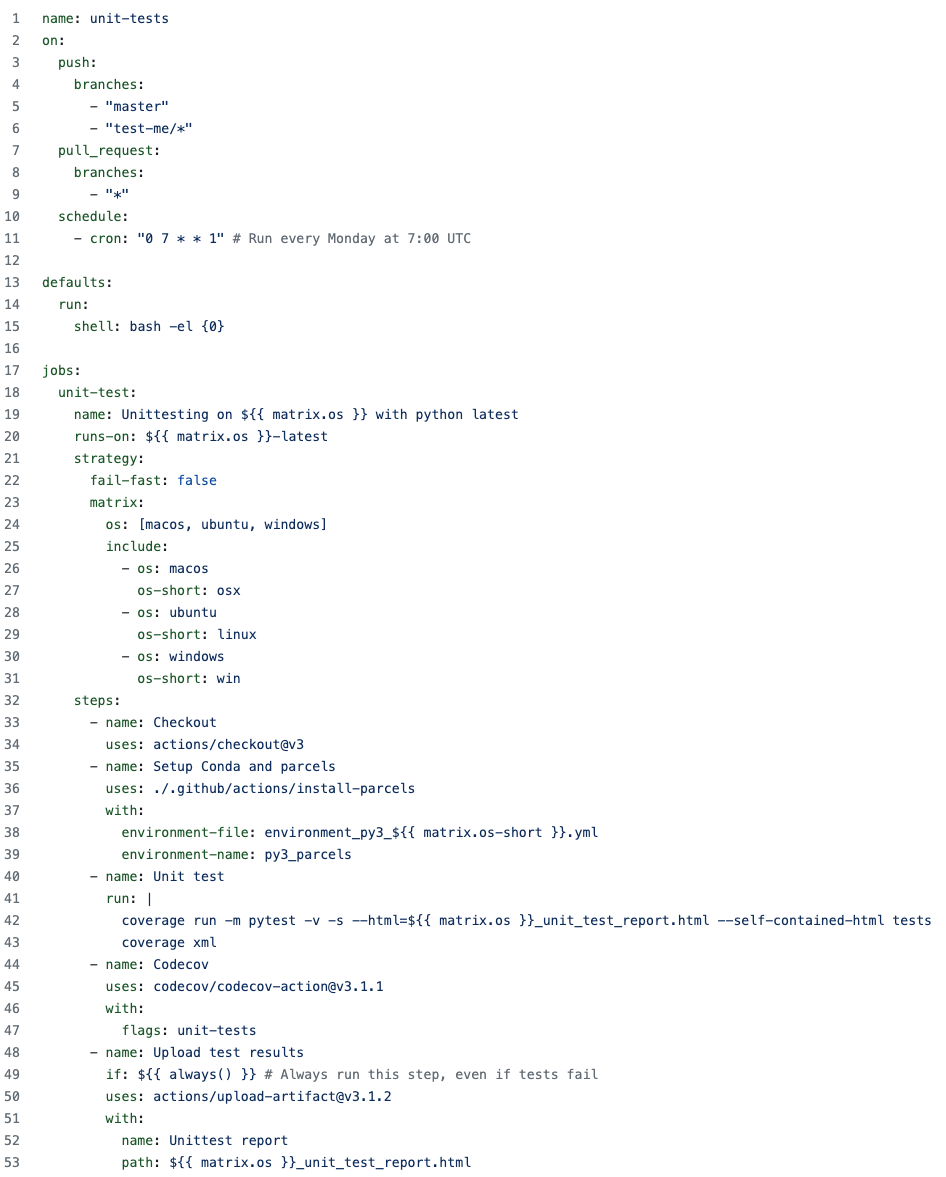
\includegraphics[scale=0.4]{JAI 2023/figures/parcels-automated-tests.png}
    \caption{Fluxo de trabalho automatizados no repositório do \RSw \texttt{Parcels}}
    \label{fig:automatizacao:parcels}
\end{figure}

\subsubsection*{P11. Automatização de tarefas} 

Durante o desenvolvimento de software muitas tarefas são realizadas de forma repetitiva. A automatização permite que essas tarefas sejam executadas de forma rápida e consistente por meio de \textit{scripts}, ferramentas ou sistemas automatizados.
Além dos testes, outras tarefas podem ser automatizadas para ajudar a encontrar e investigar \textit{bugs} mais rapidamente, melhorar a qualidade do software e reduzir o tempo para validação e lançamento de versões do software. 
A automatização pode ser configurada para executar diferentes tipos de testes (unitários, integração), para analisar o código-fonte em busca de problemas de estilo, convenções de codificação ou más práticas, entre outras tarefas. 

\noindent \textbf{Exemplo.}
A Figura~\ref{fig:automatizacao:parcels} mostra um exemplo de automatização de tarefas 
e apresenta um arquivo com a definição de passos para a execução dos testes unitários do \RSw \texttt{Parcels}.

%Ferramentas para analisar a qualidade do código (bugs, erros de estilos, por exemplo).

%Ilustrar com outro software de pesquisa. Sugestão? Colocar figura da tela, mostrando a infra para testes nesse projeto.

%\begin{figure}[htb]
%    \centering
%    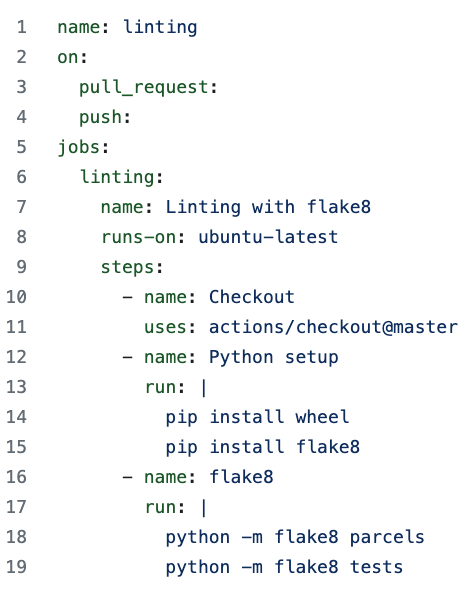
\includegraphics[scale=0.30]{JAI 2023/figures/parcels-automated-lint.png}
%    \caption{Lista de fluxos de trabalho automatizados no repositório do software de pesquisa Parcels}
%    \label{fig:automatizacao:parcels}
%\end{figure}

\subsubsection*{P12. Integração e implantação contínuas} 

\textit{Integração Contínua} (``Continuous Integration'') e \textit{Implantação Contínua} (``Continuous Deployment'') são práticas de automação no desenvolvimento de software que possibilitam a entrega rápida e confiável de um software. 
Na integração contínua, as mudanças são automaticamente verificadas e integradas, permitindo que os problemas sejam detectados e corrigidos mais cedo no processo de desenvolvimento. A implantação contínua permite que as mudanças sejam disponibilizadas automaticamente para os usuários.

%Como utilizar ferramentas de CI/CD no desenvolvimento de
%software de pesquisa?
Para configurar um sistema de integração contínua é necessária a configuração de uma ferramenta, como \textit{Jenkins}, \textit{CircleCI}, \textit{Travis CI} ou \textit{GitHub Actions}, para monitorar o repositório do software e executar automaticamente testes e tarefas de verificação.
A Figura~\ref{fig:ci:cd:parcels} mostra um \textit{pull request} no repositório do \RSw \texttt{Parcels}. 
O projeto implementa integração contínua e, a cada \textit{pull request} nesse repositório, 
tarefas automatizadas são executadas, como testes unitários e de integração e uso de uma ferramenta de análise de código-fonte (\textit{linter}) para identificar possíveis problemas no código. 
Como as tarefas são obrigatórias, o código não poderá ser incorporado ao \textit{branch} principal se alguma das atividades falhar. Na Figura~\ref{fig:ci:cd:parcels}, podemos observar que  os testes unitários falharam.

\begin{figure}[tb]
    \centering
    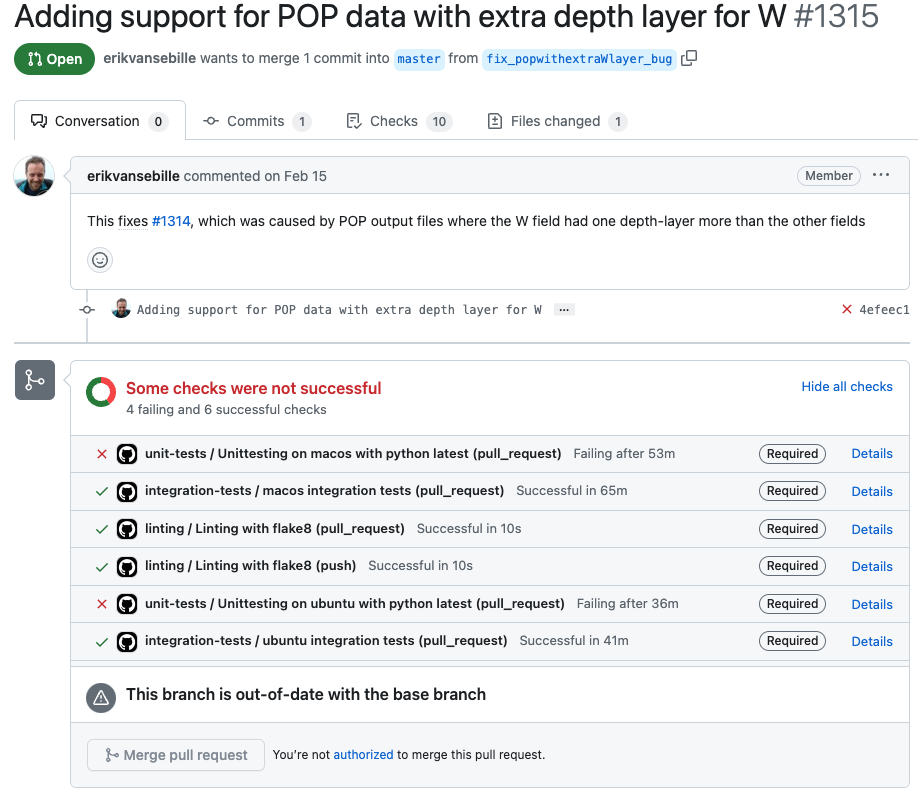
\includegraphics[scale=0.4]{JAI 2023/figures/parcels-pr.png}
    \caption{\textit{Pull request} com testes unitários falhando no repositório do projeto Parcels}
    \label{fig:ci:cd:parcels}
\end{figure}

\begin{figure}[tb]
    \centering
    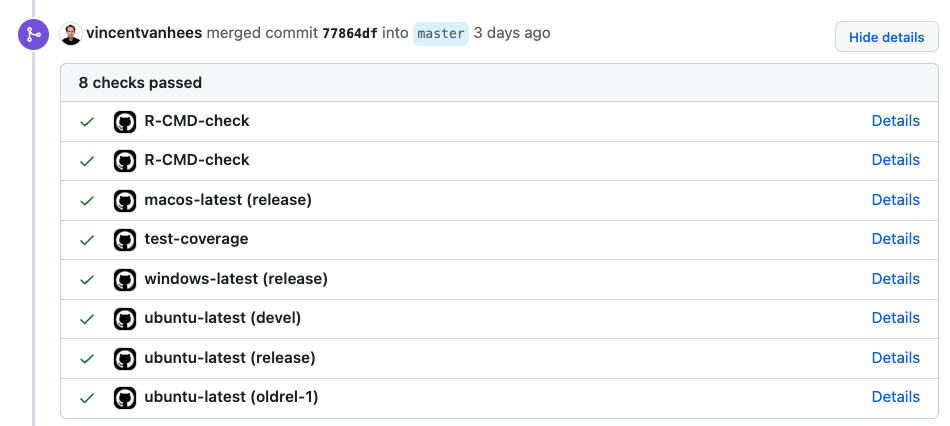
\includegraphics[scale=0.40]{JAI 2023/figures/ggir-ci-cd.png}
    \caption{Tarefas automatizadas executadas após a incorporação de um \textit{pull request} no repositório do \RS.}
    \label{fig:ci:cd:ggir}
\end{figure}

Os \textit{pipelines} de implantação contínua são fluxos de trabalho automatizados que ajudam a \textit{implantar novas versões do software em diferentes ambientes}. Eles podem ser criados usando ferramentas como \textit{Docker}, \textit{Kubernetes}, \textit{GitLab CI/CD} e \textit{CircleCI}.
Para exemplificar a prática, a Figura~\ref{fig:ci:cd:ggir} mostra as tarefas automatizadas realizadas quando um \textit{pull request} é incorporado ao projeto na \textit{branch} principal. O projeto é o \RSw GGIR\footnote{\url{https://github.com/wadpac/GGIR}}, que converte dados brutos de dispositivos vestíveis em relatórios para pesquisadores que investigam a atividade física diária e o sono humano. Após a aprovação do \textit{pull request}, as tarefas automatizadas são executadas e o lançamento da versão.

Ao adotar essas práticas de integração e implantação contínuas no \RS, a confiabilidade do software será maior e a entrega de novas funcionalidades será mais rápida e segura.

%Ilustrar com outro software de pesquisa. Sugestão? Colocar figura da tela, mostrando a infra para CI/CD nesse projeto.

% Movi pra parte de Avaliação
%\noindent \textbf{\texttt{Software Mosyn}}.
%Não há integração contínua. Por ser um plugin instalado manualmente no MATLAB, a implantação contínua não é viável.

\subsubsection*{P13. Lançamento de versões} 

O \textit{lançamento de versões} é importante durante o desenvolvimento de \RSw sustentável para permitir a rastreabilidade das mudanças e permitir que a pesquisa seja reproduzida a partir de uma versão específica do software. O lançamento de versões envolve a marcação de pontos específicos no histórico do código-fonte para representar marcos no desenvolvimento do software. Os repositórios de código fonte fornecem vários recursos que apoiam o lançamento de versões.

Uma estratégia comum é o uso de \textit{tags} (etiquetas), ou marcadores atribuídos a um \textit{commit} para identificar uma versão específica do software. 
As \textit{tags} podem ser usadas para identificar versões estáveis, versões de correção de \textit{bugs}, pontos de lançamento importantes ou algum \textit{milestone} (marco) no desenvolvimento do projeto. Por exemplo, uma \textit{tag} pode ser criada para indicar a primeira versão funcional do software (``versão~1.0'').

Outro recurso importante é o uso de \textit{releases} (lançamentos), com software empacotado e disponibilizado para os usuários. 
\textit{Pacote} (\textit{package}) é o termo utilizado para representar um conjunto organizado de arquivos e recursos relacionados que são distribuídos juntos como uma unidade coesa. O pacote pode incluir o código-fonte do software, dependências, arquivos de configuração, documentação e qualquer outro componente necessário para executar ou instalar o software. A disponibilização do \RSw como pacote facilita a distribuição, instalação e utilização do software, entregando um conjunto funcional de recursos e funcionalidades para os usuários. Cada \textit{release}  pode incluir \textit{release notes} (notas de lançamento) detalhando as alterações, correções de \textit{bugs} e outras informações relevantes.

O nome da versão geralmente segue uma convenção numérica ou alfanumérica, como ``1.0'', ``2.3'' ou também pode incluir um identificador descritivo, como ``versão beta'' ou ``versão alpha''. 
O versionamento semântico\footnote{\url{https://semver.org/lang/pt-BR}} é uma prática comum fortemente recomendável ao adotar e usar versionamento para gerenciar as \textit{releases} do \RS.
%
O \textit{escopo de uma versão} engloba as alterações e atualizações contidas na versão específica, inseridas pelos \textit{commits} incluídos desde a versão imediatamente anterior até a versão sendo lançada. 
Recomenda-se incluir na descrição da \textit{release} informações sobre o seu escopo, por exemplo, funcionalidades adicionadas, problemas resolvidos, melhorias de desempenho, atualizações de segurança e outros detalhes relevantes. Essas informações ajudam a comunicar claramente o que uma determinada versão oferece aos usuários.

\noindent\textbf{Exemplo.}
O \RSw \texttt{Parcels} está em um repositório público e utiliza as funcionalidades de \textit{tags} que descrevem o escopo da versão nos lançamentos de versões.
A Figura~\ref{fig:tags:parcels} apresenta a lista de \textit{tags} no repositório e a Figura~\ref{fig:release:parcels} mostra as notas do lançamento de uma versão do projeto.

\begin{figure}[tbp]
    \centering
    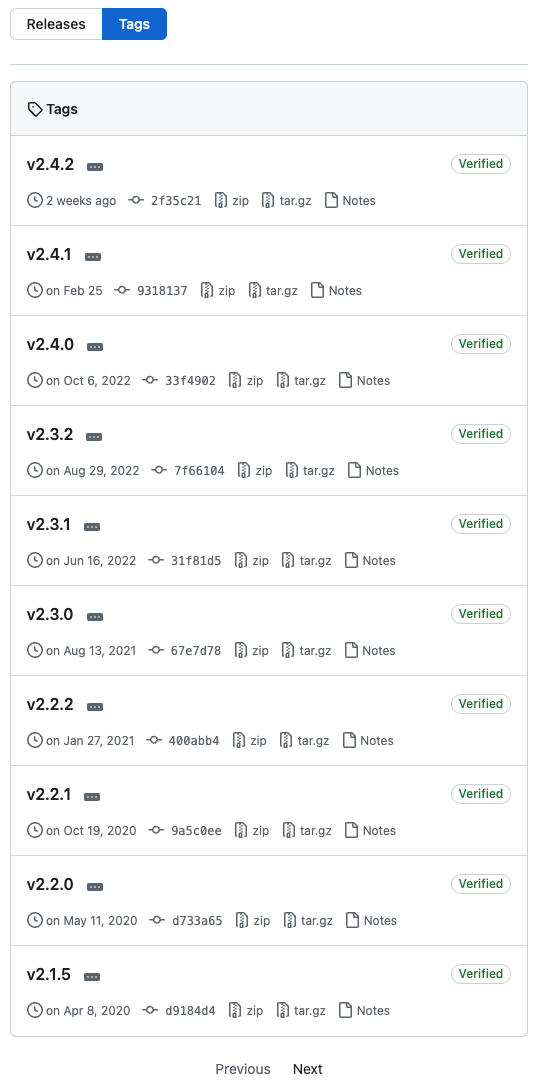
\includegraphics[scale=0.5]{JAI 2023/figures/parcels-tags.png}
    \caption{Lista de \textit{tags} no repositório do software de pesquisa \texttt{Parcels}.}
    \label{fig:tags:parcels}
\end{figure}

\begin{figure}[tbp]
    \centering
    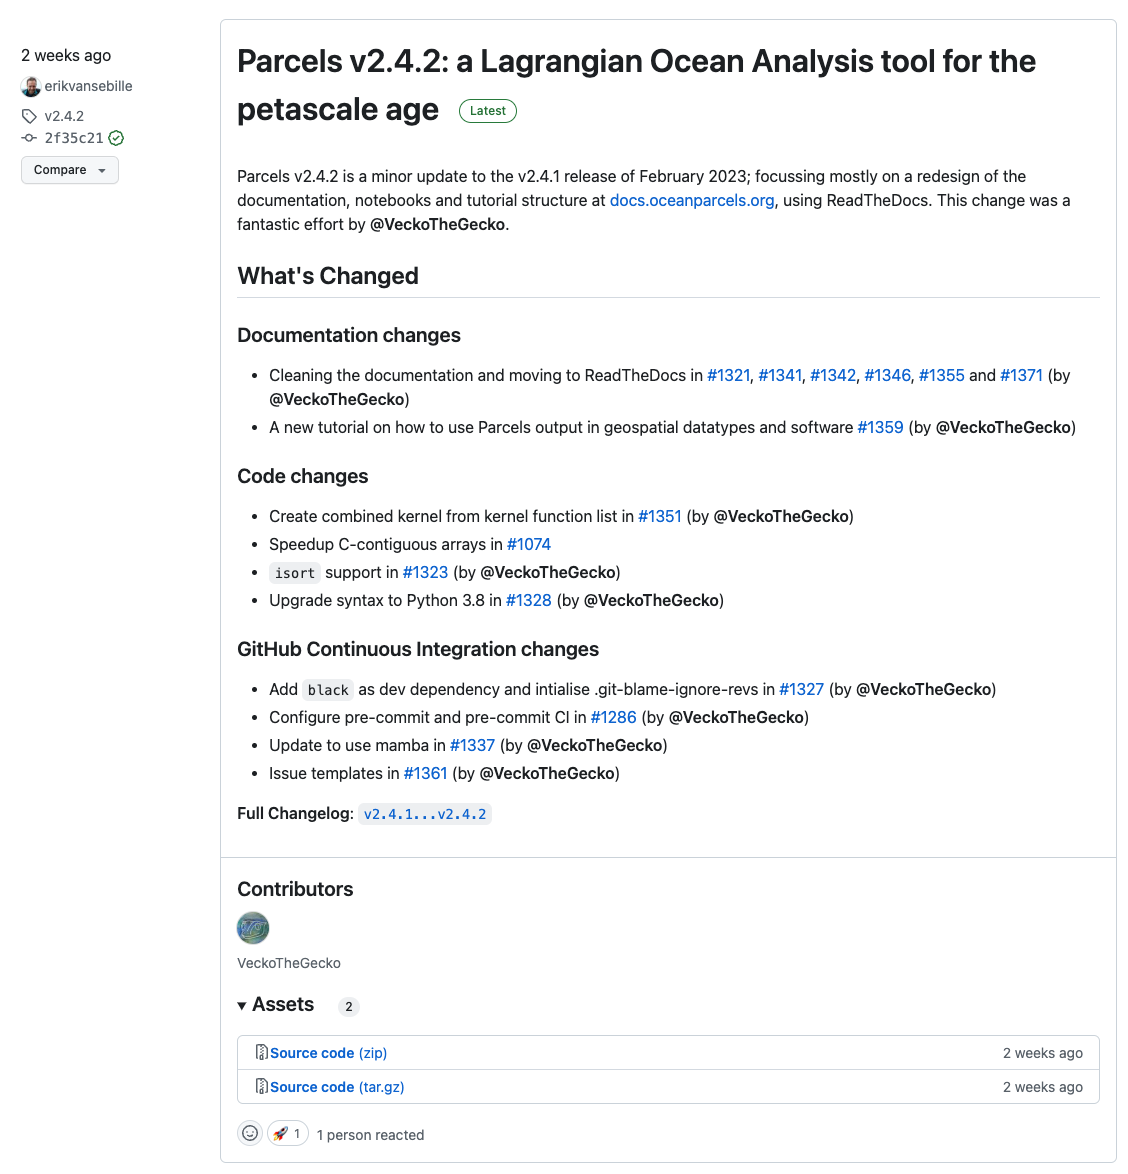
\includegraphics[scale=0.40]{JAI 2023/figures/parcels-release.png}
    \caption{Notas de lançamento de uma versão no repositório do software de pesquisa Parcels.}
    \label{fig:release:parcels}
\end{figure}

%------------------------------------%

\begin{comment}
\subsection{Aspectos de Comunidade}
%“I have my first pull request, and the beginning of a community. What now?” Returns in more depth to issues of licensing and release management, with added information about community-building and sustainability concerns.

\textit{Quero usuários:} Release your software; Provide user documentation; Easy installation; Provide issue tracker.

\textit{Quero contribuidores:} 
Provide development documentation; Provide a means of communication; Implement and add a code of conduct; 
Contribution guideline.

%\textit{Quero reconhecimento:} forma de citar software ...
\end{comment}

%------------------------------------%
\subsection{Reconhecimento}

As boas práticas que promovem a sustentabilidade técnica do \RSw podem atrair usuários e contribuidores para o software.
%
As práticas apresentadas a seguir estão relacionadas com o reconhecimento da relevância do \RSw para outros pesquisadores e da necessidade de sua divulgação e citação apropriadas.

\subsubsection*{P14. Comunidade do projeto} 

Em geral, o \RSw é desenvolvido por indivíduos ou em pequenos grupos de pesquisa dentro de uma única instituição, resultando em protótipos para atender às suas próprias necessidades, por exemplo, validar uma hipótese ou apoiar atividades da pesquisa.
%
Criar uma comunidade em torno de um \RSw é essencial para aumentar a adoção e colaboração, ampliando seu impacto na comunidade científica. 
Além disso, a comunidade ajuda na identificação e correção de problemas e traz novas sugestões para o desenvolvimento do software. 

Uma comunidade ativa e engajada promove a colaboração entre pesquisadores e desenvolvedores de diferentes instituições e áreas de pesquisa. Tal engajamento facilita a troca de ideias, a discussão de problemas, a identificação de \textit{bugs}, a proposição de novas funcionalidades, a implementação de melhorias e novas funcionalidades para o software. 
Outra vantagem da comunidade é realizar revisão por pares do código-fonte, documentação e resultados produzidos pelo software. Essas revisões ajudam a garantir a qualidade e a confiabilidade do software. A diversidade de perspectivas e experiências na comunidade contribui para um processo de desenvolvimento mais completo. Além disso, a existência de uma comunidade ativa em torno do \RSw pode aumentar sua sustentabilidade no longo prazo. 
Com uma base de usuários e desenvolvedores engajados, o software tem maior probabilidade de receber suporte financeiro, recursos e atualizações contínuas, facilitando sua disponibilidade e relevância para outros pesquisadores.

%- Estratégias para envolver usuários e colaboradores, estabelecer diretrizes para participação, reconhecer e valorizar as contribuições e \textit{manter canais de comunicação, como fóruns de discussão, listas de e-mails, chat e eventos}.

Para envolver usuários e colaboradores em um \RS, é importante estabelecer diretrizes claras, reconhecer e valorizar as contribuições, disponibilizar canais de comunicação, organizar eventos e atividades, fornecer documentação detalhada e acessível e incentivar a colaboração ativa.

%É mais provável que os usuários e colaboradores se sintam encorajados a participar se o projeto estabelecer 
As diretrizes que orientam a participação na comunidade abordam aspectos sobre como contribuir com código, como reportar problemas e participar em discussões. Idealmente, o projeto deve disponibilizar um código de conduta e um guia sobre como contribuir.
Quando definidas e seguidas, diretrizes ajudam a criar um ambiente colaborativo e respeitoso. 
%
Outra estratégia essencial é reconhecer e valorizar as contribuições dos usuários e colaboradores. Com agradecimentos públicos, inclusão de nomes nos créditos do projeto, menções em publicações relacionadas ao \RSw e outros gestos de reconhecimento, incentivam-se o engajamento contínuo e a motivação para continuar colaborando com o projeto.

Para facilitar a interação entre os membros da comunidade é fundamental disponibilizar \textit{canais de comunicação}, como fóruns de discussão online, listas de e-mails, salas de bate-papo e plataformas como GitHub e GitLab. 
Esses canais permitem que os colaboradores obtenham suporte técnico, compartilhem ideias, troquem experiências e contribuam com melhorias no \RS. Também é possível promover a interação direta entre os membros da comunidade com a organização ou participação em conferências, workshops, treinamentos e eventos.

Para incentivar a colaboração ativa dos usuários é importante a identificação de tarefas específicas que precisam de contribuições, a criação de programas de mentoria para novos colaboradores, orientações claras sobre como contribuir para o projeto. 
Por fim, é essencial fornecer uma documentação detalhada e acessível para que os colaboradores possam compreender e utilizar o software de forma eficaz. 

%\textbf{Suporte para reprodutibilidade?}

%\textit{Quero contribuidores:} Provide development documentation; Provide a means of communication; Implement and add a code of conduct; Contribution guideline.

\noindent\textbf{Exemplo.} 
% Um artigo de Terceiro da época do doutorado?
A ferramenta \texttt{flosssearch} foi implementada em PHP, por conveniência e experiência do desenvolvedor, pensando na construção de uma comunidade que, no futuro, poderia transformar \texttt{flosssearch} em um produto.
Porém não há políticas ou recomendações definidas para os membros da comunidade.
% Movi pra parte de Avaliação
%\noindent \textbf{\texttt{Software Mosyn}}.
%Apenas o usuário dono do repositório submeteu \textit{commits} e \textit{pull requests} no projeto. A página do projeto não apresenta outros usuários que adicionaram o projeto como favorito e não mostra usuários que fizeram uma cópia (\textit{fork}) independente do projeto.

A plataforma GitHub apresenta suas políticas e recomendações para os membros da comunidade\footnote{\url{https://docs.github.com/en/site-policy/github-terms/github-community-guidelines}}, incentivando-os a
moderar seus projetos sempre que possível e denunciar qualquer conteúdo que possa violar tais políticas.

\subsubsection*{P15. Divulgação de Software} 

%Divulgação em eventos científicos, estudos com outros pesquisadores para avaliar usabilidade da ferramenta e potencial interesse.

A divulgação do \RSw em eventos científicos e estudos com outros pesquisadores é de extrema importância. Essas oportunidades permitem que os pesquisadores compartilhem e apresentem suas soluções de software, que avaliem a usabilidade da ferramenta e potenciais interesses em comum.
 
Ao apresentar o \RSw para a comunidade acadêmica e colaborar com outros pesquisadores, é possível receber opiniões, estabelecer parcerias, trocar conhecimento e, talvez, aumentar o impacto e a adoção do software de pesquisa, impulsionando o alcance da ciência.

%Quando o \RSw for usado em artigos científicos, é preciso registrar qual a versão do software foi utilizada em cada artigo.
% Um artigo de Terceiro da época do doutorado?
\noindent \textbf{Exemplo.}
O software \texttt{flosssearch} foi utilizado e publicado em artigos científicos, tanto como instrumento da pesquisa, como produto da pesquisa. Entretanto, ainda não há informações  documentadas no repositório sobre a correspondência entre artigos publicados e versões do software.

O arquivo README do \texttt{Parcels} apresenta uma seção sobre ``manuscrito e código'', onde cita artigos publicados e a versão software usada:
\begin{quote}
The manuscript detailing the performance of \texttt{Parcels v2.4} is available at Computers \& Geosciences and can be cited as:

Kehl, C, PD Nooteboom, MLA Kaandorp and E van Sebille (2023).
\textit{Efficiently simulating Lagrangian particles in large-scale ocean flows -- Data structures and their impact on geophysical applications}, Computers and Geosciences, 175, 105322. 
https://doi.org/10.1016/j.cageo.2023.105322
\end{quote}

\subsubsection*{P16. Citação de Software} 

%Citação de \textit{Research Software} para que pesquisadores e desenvolvedores recebam crédito por seu trabalho.
A boa prática científica exige que o \RSw mencionado em publicações científicas seja mantido para reprodutibilidade e verificação de resultados científicos.
%
Citar um software de pesquisa é uma forma de reconhecer e dar visibilidade aos autores e ao próprio software, possibilitando que outros pesquisadores o localizem e eventualmente reusem. Entretanto, 
a citação de software em publicações científicas ainda não é uma prática comum entre cientistas, mas padrões de citação têm sido propostos e adotados. 

Em seu artigo ``Recognizing the value of software: a software citation guide'',  \cite{katz:citation:format} apresentam instruções simples sobre como o software pode se tornar citável e destacam que o uso de identificadores persistentes (PIDs) e metadados descritivos são elementos essenciais da citação de software. 
Informações sobre autoria, nome, local de publicação, data de publicação e identificador do software são consideradas obrigatórias.
%
Adicionalmente, alguns estilos de citação pedem uma descrição da citação entre colchetes. Para software, pode-se usar \textit{[Computer software]}.
A Tabela~\ref{tab:citation:format} apresenta o formato de citação de software proposto por~\cite{katz:citation:format}.

\begin{table}[htb]
    \centering
        \caption{Formato de Citação de Software \cite{katz:citation:format}.}
    \label{tab:citation:format}
    \begin{tabular}{p{2.5cm}|p{11.5cm}}
    \hline
        \textbf{Informação} & \textbf{Descrição} \\
    \hline
        \textbf{Criador(es)} & Autor(es) ou projeto que desenvolveram o software \\
        \textbf{Título} & Nome do software \\
        \textbf{Local} & Local de publicação do software, por exemplo, um arquivo ou repositório que fornece identificadores persistentes. \\
        \textbf{Data} & Data em que o software foi publicado, por exemplo, a data associada a um lançamento ou versão do software.\\
        \textbf{Identificador} &  Um apontador resolvível para o software,  de preferência um PID que leve para uma página contendo metadados descritivos sobre o software, semelhante a um DOI. \\
    \hline
    \end{tabular}
\end{table}

%What is a CITATION.cff file?
%Citation File Format (CFF) (Druskat et al. 2021) (v1.2.0) are plain text files with human- and machine-readable citation information for software (and datasets). Code developers can include them in their repositories to let others know how to correctly cite their software.
%This format is becoming popular within the software citation ecosystem. Recently GitHub, Zenodo and Zotero have included full support of this citation format (Druskat 2021). GitHub support is of special interest:

%
O formato \textit{Citation File Format} (CFF)\footnote{\url{https://citation-file-format.github.io}} tem se popularizado como formato e padrão para documentar como citar um projeto de software~\cite{druskat:2021}.
%
Adicionar um arquivo {\em CITATION.cff} ao repositório do \RSw pode ser uma boa forma documentar e atualizar as recomendações definidas para citação do software. 
Recentemente, Zenodo e GitHub facilitaram a adição de metadados aos repositórios e a geração de citações para esses 
repositórios~\cite{smith:2021}. 

Além disso, pode-se definir um ID persistente para o \RS, por exemplo, um DOI obtido para um artigo que apresenta o software para a comunidade (\textit{software paper}) ou ainda usar formatos mais recentes como o SWHID\footnote{\url{https://www.swhid.org}} promovido pelo projeto Software Heritage\footnote{\url{https://www.softwareheritage.org}}, uma iniciativa dedicada a coletar e preservar software em formato de código-fonte para preservação e acesso público.
%
Entretanto, \cite{katz:citation:format} recomendam que, se existir um artigo que apresenta o \RSw para a comunidade científica, ele deve ser citado como uma referência bibliográfica \textit{adicional}, mas não deve substituir a citação do software propriamente dita.

\noindent\textbf{Exemplo.} 
O \RSw \texttt{flosssearch} não definiu como deve ser citado. 
A ferramenta \texttt{Analizo} indica uma publicação que pode ser considerada como citação para o software~\cite{analizo2010} mas não apresenta uma citação de software.

%Ele foi usado em cinco estudos nos últimos quatro anos, porém os artigos científicos mencionam apenas a sua URL, sem detalhes sobre a versão utilizada. 

\begin{comment}

\begin{table}[htb]
\begin{tcolorbox}[colback=white,title=Descrição do Software de Pesquisa]
\begin{description}
    \item [\texttt{flosssearch.}] Software para apoio à busca e seleção de um projeto OSS para uso na Educação em Engenharia de Software.
    \item[Funcionalidades.] xxx.
    \item[Linguagem de programação.] PHP 5.6 (99.3\%)
    \item[Citação.] M. Brito, B. Lessa, C. Flach. "flossearch".
    \item[Versão.] 1.0
    \item[Licença.] GPL 3.0
    \item[URL.] ...
\end{description}
\end{tcolorbox}
\end{table}
   
\end{comment}


% Para software, essas mudanças incluem a publicação de artigos sobre software, tanto em periódicos gerais quanto em periódicos especializados em artigos sobre software (por exemplo, Journal of Open Source Software Smith et al., 2018), bem como chamadas para citação direta de software ( Smith et al., 2016) juntamente com orientações para essas citações (Katz et al., 2021). 
% O software, como um objeto digital, também tem a vantagem de ser geralmente armazenado como uma coleção de arquivos, muitas vezes em um repositório de software. Esse fato significa que é relativamente simples adicionar um arquivo adicional contendo metadados sobre o software, incluindo criadores e contribuições, em um dos vários estilos possíveis (Wilson, 2013; Druskat, 2020; Jones et al., 2017). 
% O GitHub recentemente reforçou esse esforço, o que facilitou a adição desses metadados aos repositórios e a geração de citações para esses repositórios (Smith, 2021).


%-----------------------------------------------%
\section{Avaliação do \RSw \texttt{MoSyn} }
\label{section:casesstudy:mosyn}

Nesta seção, apresentamos os resultados de um estudo exploratório conduzido com um grupo de pesquisa da área de Física com o objetivo de identificar problemas relacionados ao \RSw desenvolvido pelo grupo, fazer uma caracterização inicial da sustentabilidade 
e aderência aos princípios FAIR de um \RSw e recomendar boas práticas para torná-lo mais sustentável e aberto.

\subsection{Entrevista com Pesquisador}

A primeira atividade do estudo foi a realização de uma entrevista com um pesquisador sênior e líder de grupo de pesquisa da área de Física Aplicada, com mais de 30 anos de experiência. 
%O entrevistado realizou um breve curso técnico relacionado à computação.
Seu interesse no desenvolvimento de \RSw é motivado pelo desejo de utilizar a computação como ferramenta para avançar o conhecimento em sua área de pesquisa.
As respostas forneceram importantes considerações sobre o uso de práticas de sustentabilidade no \RSw desenvolvido por seu grupo.

De forma geral, as opiniões do pesquisador endossam fortemente o uso de \RSw sustentável para o grupo de pesquisa. Ele reconhece o valor desse trabalho e o desejo de contribuir para a comunidade de pesquisa em geral.
Sua crença nos benefícios da sustentabilidade, aliada ao entusiasmo em tornar o software acessível e ao reconhecimento da importância da replicação, reforça ainda mais o apoio do pesquisador às práticas de \RSw sustentável.
Ele destaca a necessidade de mais conhecimento por parte dos desenvolvedores do grupo de pesquisa.
Os integrantes do grupo valorizariam ter suporte para entender e implementar essas práticas de forma eficaz. 

Os resultados também destacam as considerações e dilemas relacionados ao desejo de abertura, à proteção de suas contribuições intelectuais e ao receio de comprometer a integridade e a credibilidade de sua pesquisa ao compartilhá-la prematuramente.
A falta de familiaridade dos desenvolvedores de \RSw com as melhores práticas de desenvolvimento de código também é considerada uma barreira. 
O grupo de pesquisa inclui pesquisadores com formação acadêmica em diferentes áreas, 
sendo que sua \textit{expertise} principal está nas respectivas áreas de pesquisa, e não na engenharia de software.

Durante a entrevista, o pesquisador inicialmente tinha pouco conhecimento sobre as práticas de sustentabilidade em \RSw, mas demonstrou entusiasmo e aceitou as práticas apresentadas assim que foram introduzidas,  reconhecendo os benefícios e a importância da adoção de práticas de sustentabilidade no desenvolvimento de \RS. 
Outro fator de apoio identificado é o compromisso com a promoção da reprodutibilidade em sua pesquisa. 
Com os dados e o código publicamente disponíveis, a pesquisa pode ser replicada e potencialmente expor quaisquer erros ou inconsistências, contribuindo para a confiabilidade e robustez do conhecimento científico como um todo.

A atitude positiva do pesquisador em relação ao \RSw sustentável reflete uma apreciação genuína pelos benefícios que ele oferece ao seu trabalho. O pesquisador deseja que seu software esteja disponível para todos, reconhecendo seu potencial para auxiliar inúmeros pesquisadores. Ele enfatiza as aplicações práticas dos resultados da pesquisa em ambientes clínicos, onde o software poderia ser usado para avaliar e tratar pessoas de forma eficaz.
Além disso, o pesquisador destaca a importância da replicação na pesquisa e o papel do software sustentável em garantir resultados precisos e confiáveis, reconhecendo que erros e \textit{bugs} são inerentes ao software. Ele e seu grupo de pesquisa estão interessados em identificar e corrigir esses problemas. O pesquisador também reconhece os benefícios dos testes automatizados na garantia de que as novas versões do software sejam confiáveis e na correção de \textit{bugs} anteriores, economizando assim tempo e esforço valiosos. O pesquisador compreende os benefícios de tornar o \RSw sustentável e de colaborar para avançar o conhecimento científico.

No final da entrevista, solicitamos que o pesquisador indicasse alguns projetos de \RSw para avaliação de  sustentabilidade. Os resultados da avaliação, reportados em um relatório técnico, com sugestão de práticas e  melhorias,
seriam enviados para o pesquisador. 
%
Para a primeira avaliação de sustentabilidade, escolhemos o software \texttt{MoSyn}\footnote{\url{https://github.com/mpnetto/MoSyn}}, um aplicativo para análise de grafos variáveis no tempo.

\subsection{Avaliação da Sustentabilidade}

O \RSw \texttt{MoSyn} é um aplicativo baseado em MATLAB, projetado para a análise de grafos variantes no tempo (TVGs) e suas medidas associadas. A ferramenta fornece uma estrutura modular com várias classes e funções para lidar com diferentes aspectos da análise, como configuração, recursos gráficos e gerenciamento de projetos.

A Tabela~\ref{tab:ssi:criteria:garcia} apresenta um resumo da avaliação da sustentabilidade do software \texttt{MoSyn}.
A seguir, apresentamos trechos do \textit{Relatório de Avaliação} do software \texttt{MoSyn} com referências às práticas apresentadas na Tabela.

\begin{table}[htbp]
    \caption{Sustentabilidade do software \texttt{MoSyn}.}
    \centering
    \small
    \begin{tabular}{p{0.5cm}|p{4.8cm}|c|p{6cm}}
    \hline
       \textbf{P} & \textbf{Descrição} & \textbf{Atende?} & \textbf{Comentário}\\
       \hline
        P1 & O projeto está hospedado em um repositório público  & Sim & O software está disponibilizado em um repositório público no GitHub \\
        P2 & O software implementa controle de versão  & Sim & O controle de verão é implementado por utilizar o GitHub como plataforma de hospedagem \\
        P3 & Uma licença de software foi adotada  & \textit{Parcialmente} & Um arquivo declarando a licença MIT. Porém não está claro se as permissões se aplicam a qualquer arquivo fonte no repositório \\
        P4 & O software está publicado formalmente e apresentam um DOI & \textit{Não} & O repositório não menciona um DOI associado a ele mas pode ser encontrado no GitHub pelo nome \\
        P5 & A estrutura de arquivos comunica a finalidade dos elementos do projeto  & Sim & A estrutura de pastas está organizada de forma descritiva e permite inferir o conteúdo \\
        P6 & Adota formatos de dados e interfaces comuns  & Sim & Apesar de não haver documentação explícita, o software utiliza o formato de entrada e saída que facilita a integração com o MATLAB \\
        P7 & A documentação apresenta uma visão geral sobre o software & \textit{Parcialmente} & O projeto utiliza o \textit{GitHub pages} mas as informações estão incompletas e algumas URLs direcionam para um destino não válido. \\
        P8 & O software implementa testes & \textit{Não} & Não há testes automatizados para o software \\
        P9 & O código é revisado antes de ser incorporado ao código  & \textit{Parcialmente} & Todos os \textit{pull requests} listados no repositórios foram aprovados pelo próprio autor, sugerindo que não houve revisão de código por outra pessoa \\
        P10 & Disponibiliza e usa \textit{issue tracker}  & Sim & O projeto aproveita a funcionalidade de rastreamento de \textit{bugs} e tarefas disponível no GitHub \\
        P11 & As tarefas repetitivas são automatizadas  & \textit{Não} & Não encontramos tarefas automatizadas no projeto \\
        P12 & Há integração e implantação contínua  & \textit{Não} & Não há integração contínua. Por ser um plugin instalado manualmente no MATLAB, a implantação contínua não é viável \\
        P13 & O software faz lançamento de versões  & \textit{Não} & O projeto não utiliza a funcionalidade de lançamento de versões no repositório do GitHub \\
        P14 & Há evidência de uma comunidade (presente ou futuro) & \textit{Não} & Há apenas um desenvolvedor como autor \\ 
        P15 & O software é divulgado em eventos científicos  & \textit{Não} & Não encontramos divulgação em eventos científicos \\
        P16 & O software é citado em publicações científicas  & \textit{Não} & Não encontramos citação do software em publicações. \\
    \hline
    \end{tabular}
    \label{tab:ssi:criteria:garcia}
\end{table}

% https://github.com/mpnetto/MoSyn



%------------------------------------%
\subsection*{\# Relatório de Avaliação da Sustentabilidade do Software \texttt{MoSyn}}

\noindent \textbf{\#\# Práticas Básicas}

O software \texttt{MoSyn} esteve hospedado em um repositório público desde o início de seu desenvolvimento (\textbf{P1}).
Apesar da hospedagem do \RSw no GitHub
e uso das facilidades da plataforma,
um backup periódico tem sido realizado em um dispositivo de armazenamento do grupo de pesquisa, mantido nas instalações do grupo.
%
No GitHub a identidade do software é clara e única: o nome público do software é \texttt{MoSyn}. Apesar de ter um arquivo README.md, não há uma descrição do projeto que facilite sua indexação nos mecanismos de busca.
%. Inicialmente, o repositório não incluía muitos metadados. Quatro meses após a entrevista com um pesquisador do grupo foram incluídos os arquivos descrevendo o software, a licença e informações sobre como contribuir e o código de conduta. Alguns metadados estão faltando, como lista de autores e versões do software identificando o que está presente. O software também não apresenta um DOI, mas pode ser encontrado no GitHub pelo nome. Apesar de ter um arquivo README.md, não há uma descrição do projeto que facilite sua indexação nos mecanismos de busca.  Não há uma página ou site dedicado para sua divulgação.

Por estar hospedado no GitHub, \texttt{MoSyn} possui suporte para controle de versão (\textbf{P2}). 
Inicialmente, o repositório do projeto não apresentava a licença de software (\textbf{P3}). Após quatro meses da realização da entrevista com o pesquisador sênior do grupo, 
houve um \textit{commit} no repositório do software para a inclusão do arquivo  \textit{LICENSE}, descrevendo a licença escolhida, porém sem deixar claro se as permissões se aplicam a qualquer arquivo fonte do repositório.
A licença atribuída ao software \texttt{MoSyn} é a MIT\footnote{\url{https://opensource.org/license/mit/}}, um licença usada em projetos de software livre e em projeto de software proprietário.
%\noindent \textbf{Registro de Software.}
Quanto ao registro do software (\textbf{P4}),
o repositório não menciona se há um DOI associado a ele. Além disso, não encontramos uma referência para o software \texttt{MoSyn} no Zenodo.

\noindent \textbf{\#\# Organização do Projeto}

%\noindent \textbf{Estrutura do projeto.}
O repositório do \texttt{MoSyn} possui uma estrutura de arquivos (\textbf{P5}) bem definida, e usa nomes auto-explicativos para pastas e arquivos que facilitam a compreensão do propósito e utilidade do \RS.
%\noindent \textbf{Padronização}.
O software \texttt{MoSyn} também se preocupa com padronização (\textbf{P6}) visto que é uma aplicação que depende do software MATLAB\footnote{\url{https://www.mathworks.com/products/matlab.html}}, uma plataforma paga para programação e computação numérica usada por engenheiros e cientistas para analisar dados, desenvolver algoritmos e criar modelos.
Assim, o \texttt{MoSyn}
utiliza formatos de entrada e saída que facilitam a integração com o MATLAB.

%\noindent \textbf{Documentação.}

No \texttt{MoSyn}, a preocupação com documentação do software  (\textbf{P7}) ainda é incipiente e voltada para usuários do software.
Inicialmente, o repositório não tinha qualquer documentação. Quatro meses após a entrevista realizada com o pesquisador, um arquivo \textit{README} foi adicionado ao repositório com descrição da ferramenta, lista de funcionalidades, informações sobre utilização e contribuição e licença utilizada pelo software (\textbf{P7}). Os autores do software não estão listados em um arquivo, mas é possível identificar as pessoas que contribuíram com o software a partir de informações sobre autores das mudanças registradas pelo sistema de controle de versão (\textit{commits}). 
Finalmente, os desenvolvedores deram início à construção de um site para publicação de informações sobre o projeto de pesquisa e o software usando o \textit{GitHub Pages}. 
% mas não há muitas informações e ao tentar acessar alguns links mencionados eles direcionam para uma página não existente, dificultando o acesso ao conteúdo referenciado.

\subsection*{\#\# Qualidade}

%\noindent \textbf{\#\# Testes}
O \textit{MATLAB Test}\footnote{\url{https://www.mathworks.com/products/matlab-test.html}} é um conjunto de ferramentas para o desenvolvimento, gerenciamento, análise e teste de aplicações MATLAB.
Entretanto, o \RSw \texttt{MoSyn} ainda não implementa testes de software automatizados
(\textbf{P8}). Vale destacar que as ferramentas do \textit{MATLAB Test}, assim como o MATLAB, são produtos de software fechados e que requerem assinaturas pagas. 


%\noindent \textbf{Revisão de código.}
Considerando que o software \texttt{MoSyn} está publicado no GitHub, é possível realizar a revisão de código (\textbf{P9}) colaborativamente, utilizando a infraestrutura oferecida pela plataforma.  
%fazer \textit{pull requests} e a realização de revisão de código. 
Porém, até o dia da avaliação do \RS, todos os pedidos de mudança no código (\textit{pull requests}) listados no repositório foram aprovados pelo próprio autor, sugerindo que não houve revisão de código por outra pessoa.

\noindent \textbf{\#\# Gerência}

%\noindent \textbf{Rastreador de tarefas e bugs.}
O software \texttt{MoSyn} está hospedado no GitHub e conta com o seu rastreador de tarefas e \textit{bugs} nativo (\textbf{P10}). 
O \textit{GitHub Docs}\footnote{\url{https://docs.github.com/pt}}, apresenta uma breve introdução sobre como reportar um problema usando o rastreador de tarefas. 
Entretanto, o rastreador nativo do GitHub ainda não foi utilizado no projeto \texttt{MoSyn}.
%\noindent \textbf{Automatização de tarefas.}
Não foram encontradas tarefas automatizadas ou indício de automatização de tarefas (\textbf{P11}).
Por fim, não há suporte para integração e implantação contínuas (\textbf{P12}). Por ser um \textit{plugin} instalado manualmente pelo usuário no MATLAB, tais práticas não são viáveis.

%\noindent \textbf{Lançamento de versões.}
O projeto não segue a prática de lançamento de versões (\textbf{P13}) no repositório do GitHub. As funcionalidades de 'Releases' e 'Tags' que facilitariam a referência e a descrição das funcionalidades e \textit{bugs} incluídos naquela versão específicas não são utilizadas.
Apesar de não realizarem lançamentos oficiais de versões, se fosse necessário citar o \RSw em um artigo, os autores poderiam fazer referência a um \textit{commit} específico no repositório do projeto.
No histórico do projeto, vimos que um \textit{commit} com a mensagem ``mosyn 2.0'' foi incorporado quatro meses após a entrevista. 
Essa mensagem sugere uma intenção de indicar uma alteração significativa no projeto e associar um número de versão.

\subsection*{\#\# Reconhecimento}

%\noindent \textbf{Comunidade do projeto.}
O projeto ainda não possui uma comunidade (\textbf{P14}).
Apenas o usuário dono do repositório submeteu \textit{commits} e \textit{pull requests} no projeto. A página do projeto no GitHub não apresenta outros usuários que adicionaram o projeto como favorito e não mostra usuários que fizeram uma cópia independente (\textit{fork}) do projeto.

%\noindent \textbf{Divulgação de Software.}
Não encontramos artigos ou outras formas de divulgação do \RSw em eventos científicos (\textbf{P15}). % Perguntar a GARCIA.
O software \texttt{MoSyn} / MATLAB é mencionado e foi usado em uma dissertação de mestrado na área de Saúde
%\footnote{\url{https://repositorio.ufba.br/bitstream/ri/35598/1/dissertacao_de_mestrado_-_thaise_g._l._de_o._toutain.pdf}}
para extrair índices de redes funcionais cerebrais (RFC) para análise estatística~\cite{toutain}. 
Entretanto, não encontramos no texto da dissertação um identificador ou referência para o software ou para a versão usada.
%\noindent \textbf{Citação de Software.}
Também não encontramos citação do software em publicações e na dissertação mencionada (\textbf{P16}), nem informações sobre como o software deveria ser citado.

\subsection{Avaliação de \textit{FAIRness}}

As Tabelas~\ref{tab:fairness:garcia:f}, \ref{tab:fairness:garcia:a} e~\ref{tab:fairness:garcia:ir} apresentam uma avaliação preliminar de \textit{FAIRness} do software \texttt{MoSyn}. 
Cada linha da tabela apresenta um princípio, sua descrição, indicação se o software atende ou não ao princípio, e uma justificativa se procedente. Nas tabelas, destacamos as linhas em que o software \textit{não} atendeu ou atendeu \textit{parcialmente} ao princípio.
A seguir, discutimos como \RSw incorporou os princípios \textit{FAIR}.

\subsection*{\# Relatório de Avaliação de \textit{FAIRness} do Software \texttt{MoSyn}}

\noindent \textbf{\#\# F: O software e seus metadados associados são facilmente encontrados tanto por humanos quanto por máquinas}

O software \texttt{MoSyn} está hospedado com uma identidade clara e única no GitHub, não globalmente e o repositório não garante a persistência do identificador se o software for movido, por exemplo (\textbf{F1}). Os componentes do software, como classes e bibliotecas, apresentam identificadores distintos (\textbf{F1.1}).  Cada versão do software pode ser unicamente identificada por um \textit{hash de commit} e, a partir dele, é possível recuperar os metadados da versão específica (\textbf{F1.2}). O software apresenta metadados, mas não descreve as dependências, informações detalhadas sobre utilização e configuração e como deve ser a entrada e saída de arquivos (\textbf{F2}). Ao analisar os metadados a partir de um commit, é possível verificar qual versão específica do software o metadado está se referindo (\textbf{F3}). Apesar de incluir um arquivo README com informações do projeto, não há uma descrição na configuração do projeto que facilite a indexação nos mecanismos de busca (\textbf{F4}).

\noindent \textbf{\#\# A: O software e seus metadados podem ser obtidos através de protocolos padronizados}

O software \texttt{MoSyn} pode ser obtido a partir do repositório do projeto no GitHub (\textbf{A1}). Não há restrições para baixar o código-fonte, como taxas os custos relacionados à licença (\textbf{A1.1}). É possível configurar o repositório para ser acessado apenas por pessoas autorizadas (\textbf{A1.2}). Os metadados estão descritos em arquivos no repositório, então ele não seriam acessíveis caso o repositório do software não esteja mais disponíveis (\textbf{A2}).

\noindent \textbf{\#\# I: O software interopera com outros software trocando dados e/ou metadados através da interação via interface de programação de aplicativos (APIs), descrito por meio de padrões}

O software \texttt{MoSyn} é uma aplicação para MATLAB e, portanto, interopera seguindo seu padrão, mas a forma como a interação ocorre não está explicitamente descrito (\textbf{I1}). O repositório menciona o MATLAB como pré-requisito para executar a aplicação e inclui agradecimentos pela utilização de bibliotecas e recursos externos e recursos, mas não inclui referências qualificadas, como websites ou os nomes da bibliotecas e recursos externos utilizados (\textbf{I2}). 

\noindent \textbf{\#\# R: O software é tanto utilizável (pode ser executado) quanto reutilizável (pode ser compreendido, modificado, aprimorado ou incorporado a outros softwares)}

O software \texttt{MoSyn} não disponibiliza muitas informações descrevendo como reutilizar o software (\textbf{R1}). O software  está licenciado sob a licença de código aberto MIT, que permite a reutilização, mas não deixa claro se todas as partes do software seguem a mesma licença (\textbf{R1.1}). A partir dos commits e da lista de contribuidores do projeto no GitHub é possível saber quais pessoas contribuíram com o software, mas não há informações explícitas sobre como o software foi desenvolvido ou quais foram as intenções originais (\textbf{R1.2}). Os nomes e informações sobre as bibliotecas utilizadas não são mencionadas na documentação (\textbf{R2}). A comunidade MATLAB recomenda que sejam seguidas as melhores práticas de desenvolvimento de software em relação a correção, clareza e generalização e o software, em geral, atende a esses padrões (\textbf{R3}).

% https://github.com/mpnetto/MoSyn

\begin{table}[tb]
    \caption{\textit{FAIRness} no Software MoSyn -- \textit{Findable}.}
    \centering
    \small
    \begin{tabular}{p{0.9cm}|p{5cm}|c|p{5.25cm}}
    \hline
    Princ. & Descrição & Atende? & Comentário 
    \\ \hline
     F: & O software e seus metadados associados são facilmente encontrados tanto por humanos quanto por máquinas. & \textit{Parcialmente} &  \\
     F1 & O software recebe um identificador globalmente único e persistente. & \textit{Parcialmente} & O software possui uma identidade única apenas no GitHub e não é garantida a persistência. \\
     F1.1 & Aos componentes do software que representam diferentes níveis de granularidade são atribuídos identificadores distintos. & Sim & \\
     F1.2 & As diferentes versões do software recebem identificadores distintos. & Sim & \\ \hline
     F2 & O software é descrito com metadados detalhados. & \textit{Parcialmente} & O software menciona alguns metadados, mas sem muitos detalhes que permitam encontrar o software facilmente \\
     F3 & Os metadados contêm de forma clara e explícita o identificador do software que descrevem. & \textit{Parcialmente} & Os metadados não apresentam de forma clara, mas é possível obter a partir do \textit{commit} \\
     F4 & Os metadados seguem os princípios FAIR, são pesquisáveis e indexáveis. & \textit{Parcialmente} & Há informações nos arquivos do repositório, mas não há descrição na configuração do projeto para facilitar indexação \\
      \hline
    \end{tabular} \label{tab:fairness:garcia:f}
\end{table}

     
\begin{table}[tb]
    \caption{FAIRness no Software MoSyn -- \textit{Accessible}.}
    \centering
    \small
    \begin{tabular}{p{0.9cm}|p{4.9cm}|c|p{5.5cm}}
    \hline
    Princ. & Descrição & Atende? & Comentário 
    \\ \hline
     A: & O software e seus metadados podem ser obtidos através de protocolos padronizados. & \textit{Parcialmente} &\\
     A1 & O software é pode ser obtido por meio de seu identificador utilizando um protocolo de comunicação padronizado. & Sim &\\
     A1.1 & O protocolo é aberto, gratuito e universalmente implementável. & Sim &\\
     A1.2 & O protocolo permite procedimentos de autenticação e autorização, quando necessário. & Sim &\\
     A2 & Os metadados são acessíveis, mesmo quando o software não está mais disponível. & Não & Caso o software não esteja mais disponível, os metadados também ficarão inacessíveis\\
      \hline
    \end{tabular} \label{tab:fairness:garcia:a}
\end{table}

     
\begin{table}[tb]
    \caption{FAIRness no Software MoSyn -- \textit{Interoperable, Reusable}.}
    \centering
    \small
    \begin{tabular}{p{0.9cm}|p{6cm}|c|p{4.3cm}}
    \hline
    Princ. & Descrição & Atende? & Comentário 
    \\ \hline
     I: & O software interopera com outros softwares, trocando dados e/ou metadados através da interação via APIs, descrito por meio de padrões. &  &  \\
     I1 & O software lê, escreve e troca dados de acordo com padrões da comunidade relacionados ao domínio. & \textit{Parcialmente} & Não está explícito como a troca de dados ocorre com o MATLAB \\
     I2 & O software inclui referências qualificadas a outros objetos. & \textit{Parcialmente} & As referências se resumem a menção sobre utilização, sem citar nomes, websites ou detalhes dos outros objetos \\
     \hline
     R: & O software é utilizável (pode ser executado) e reutilizável (pode ser compreendido, modificado, aprimorado ou incorporado a outros softwares). & \textit{Parcialmente} & \\
     R1 & O software é descrito com uma variedade de atributos precisos e relevantes. & \textit{Parcialmente} & Não há muitas informações sobre atributos e como reutilizar o software \\
     R1.1 & É atribuída uma licença clara e acessível ao software. & Sim &  \textit{MIT License.} \\
     R1.2 & O software possui informações detalhadas de procedência. & \textit{Parcialmente} & Não há informações sobre como o software foi desenvolvido ou quais foram as intenções originais \\
     R2 & O software inclui referências qualificadas a outros softwares. & \textit{Parcialmente} & Não há informações relevantes sobre dependências. \\
     R3 & O software atende aos padrões relevantes da comunidade do domínio. & Sim & \\
      \hline
    \end{tabular} \label{tab:fairness:garcia:ir}
\end{table}

%\subsection{Discussão}

%O objetivo da avaliação do \RSw \texttt{MoSyn} não é reportar se ele é sustentável ou não é sustentável. 
% O processo de avaliar um \RSw com base nas práticas usadas no desenvolvimento inicial e manutenção contínua promove a observação e reflexão sobre o produto de software e as práticas empregadas, tanto para o desenvolvimento como para promover seu reconhecimento pela comunidade científica.


%Proposta de identificadores persistentes especifico para Software como o SWHID \footnote{https://www.swhid.org}.

%-------------------------------------------%
\section{Considerações Finais}
\label{section:conclusions}

%\subsection{Iniciativas para promover a Sustentabilidade do Software de Pesquisa} \label{subsection:initiatives}

O reconhecimento da necessidade de reprodutibilidade na pesquisa científica, bem como o advento recente da criação de comitês de avaliação de artefatos de pesquisa em conferências e periódicos levaram à recomendação para que os autores  disponibilizem dados de pesquisa, \RS, documentação e materiais usados nas publicações científicas. 
Nesse contexto, o \RSw desenvolvido deve ser sustentável para que cientistas possam entender, replicar e reproduzir pesquisas anteriores ou conduzir novas pesquisas de forma eficaz. 
O suporte à reprodutibilidade ainda demanda que o \RSw seja \textit{FAIR} -- localizável, acessível, interoperável e reutilizável, para responder às necessidades de pesquisa, presentes e futuras. 

%O desenvolvimento de um \RSw requer um ambiente que apoie a sustentabilidade. 
Entretanto, grande parte dos cientistas que escrevem \RSw ainda carecem de uma formação em boas práticas de engenharia de software, por exemplo, uso de sistemas de controle de versão, documentação adequada e testes automatizados.
Neste cenário, a sustentabilidade e outros atributos de qualidade do \RSw podem ficar comprometidos e levar a erros em conclusões científicas e falta de reprodutibilidade na pesquisa que depende do software.

Portanto, ainda que demande tempo e esforço,
uma mudança na forma como o desenvolvimento e a manutenção de \RSw são realizados é necessária, bem como a definição de um modelo de sustentabilidade de software que reconheça a importância de incorporar práticas para promover a sustentabilidade no desenvolvimento de  \RS.
Um caminho natural é investir em treinamento para cientistas de diversas áreas do conhecimento sobre conceitos, boas práticas e ferramentas
para o desenvolvimento de \RSw sustentável.

Ao adotar práticas sustentáveis, os pesquisadores podem criar oportunidades para que outros especialistas na área colaborem no desenvolvimento de seu \RS, forneçam \textit{feedback} e sugestões de melhorias. Além disso, a disseminação dos resultados da pesquisa e a divulgação do software, podem ampliar o impacto além da comunidade acadêmica, beneficiando o público em geral.

%\subsection{Ciência Aberta e Software de Pesquisa no Brasil}
% Ciência Aberta e, em especial, a .
A discussão sobre \RSw sustentável é incipiente e o tema tem sido pouco explorado pela comunidade acadêmica brasileira de Computação. 
O Simpósio Brasileiro de Engenharia de Software (SBES 2022) foi inovador ao apresentar um documento 
delineando Políticas de Ciência Aberta para o evento~\cite{flach:politicas:os}, buscando
encorajar os autores a disponibilizar os artefatos usados na pesquisa -- dados abertos anonimizados e código do \RS, e despertar o interesse na reprodutibilidade dos estudos quantitativos publicados.
O tema do SBES 2022 foi \textit{Sustentabilidade de Software}, e o título de uma das palestras convidadas, proferida pelo Prof. Daniel Katz, foi \textit{Towards Sustainable Research Software}~\cite{katz_daniel_s_2022_7140726}.

\subsection{Institutos e Associações}

Há várias iniciativas que contemplam a questão da \textit{Sustentabilidade do Software de Pesquisa} e 
o apoio a cientistas e engenheiros de software, com o objetivo de promover a adoção de boas práticas no desenvolvimento de \RSw e torná-lo mais sustentável.
%
Alguns países da Europa, América do Norte, Ásia e África têm inaugurado institutos nacionais para apoiar cientistas que desenvolvem \RSw e preparar uma nova categoria de profissionais: os engenheiros de \RS~\cite{jimenez_four_2017}. Entretanto, o Brasil ainda não investiu na criação de organizações ou institutos dedicados a este tema.

Dentre os institutos e associações pioneiros, destacam-se 
(1)~\textit{The Carpentries}\footnote{\url{https://carpentries.org}}, 
(2)~\textit{Software Sustainability Institute} (SSI)\footnote{\url{https://www.software.ac.uk}}, (3)~\textit{Research Software Engineers} (RSE)\footnote{\url{https://researchsoftware.org/}}, 
(4)~\textit{The Society of Research Software Engineering}\footnote{\url{https://society-rse.org}} e  
(5)~\textit{Netherlands eScience Center}~\cite{drost_niels_2020_4020622}. 
%, uma fundação independente baseada na Holanda para desenvolvimento e aplicação de software de pesquisa

\subsection{Cursos e Treinamentos}

Institutos, associações e outras organizações oferecem cursos e treinamentos gratuitos sobre diversos temas ligados ao \RSw e sua sustentabilidade. Recomendamos que visitem os websites e consultem o material disponibilizado.
\begin{itemize}
    \item \textit{The Carpentries}
    é um instituto que oferece treinamento em habilidades computacionais e ciência de dados para cientistas em todo o mundo.
    \item \textit{Software Carpentry} é um projeto voluntário dedicado a ensinar habilidades básicas de computação para pesquisadores~\cite{madicken_munk_2019_3264950, aleksandra_nenadic_2022_6532057}.
    \item \textit{Library Carpentry} é uma comunidade global que ensina habilidades de software e dados para pessoas que trabalham em funções relacionadas a bibliotecas e informações~\cite{madicken_munk_2019_3264950}.
    \item \textit{Netherlands eScience Center} é uma fundação independente baseada na Holanda para desenvolvimento e aplicação de software de pesquisa~\cite{drost_niels_2020_4020622}. 
    \item \textit{The Turing Way} oferece um manual para ciência de dados reprodutível, ética e colaborativa~\cite{the_turing_way_community_2022_7625728}.
\end{itemize}

%\subsection{Modelos de Avaliação}
%O \textit{Software Sustainability Institute}\footnote{\url{https://www.software.ac.uk}}

%A associação de Engenheiros de Software de Pesquisa (\textit{Research Software Engineers}\footnote{\url{https://researchsoftware.org/}} e a \textit{Society of Research Software Engineering}\footnote{\url{https://society-rse.org}})~\cite{katz_addressing_2021}.

%Diretórios de Software de Pesquisa, como o \textit{Research Software Directory}\footnote{https://research-software-directory.org} buscam facilitar a descoberta e reutilização de \textit{Software de Pesquisa}, ajudando a tornar a pesquisa mais transparente e sustentável.

% end body

%--------------------------------%

\bibliographystyle{sbc}
\bibliography{jai2023}

% Removed
%\appendix
%\section{Exemplo: ferramenta de seleção de projetos}


\url{https://github.com/seed-br/seed.select.git}

Descrever.
Para que o software? 
O problema de seleção de OSS. explicar. 
É resultado da pesquisa: o software é uma contribuição.

Ao mesmo tempo, o software deverá ser avaliado por terceiros, porque foi submetido como tool paper. Explicar.

Ao mesmo tempo, o software deverá ser usado em outras pesquisas, porque ele implementa uma funcionalidade necessária (o software é meio, instrumento).
Por exemplo, ele foi usado em um relato de experiência de aula de ES em que o projeto foi escolhido com o apoio do software.

\begin{enumerate}

    \item Permitir que os usuários filtrem projetos OSS de acordo com até 10 critérios de seleção (tamanho do projeto, linguagem de programação, entre outros).
    
    \item Permitir que usuários autenticados comentem sobre determinado projeto, possibilitando assim anotar possíveis experiências com aquele projeto. Qualquer usuário pode visualizar esses comentários.
    
    \item Allow authenticated users to evaluate a project with 1 to 5 stars to indicate the level of satisfaction in using that particular project. The average rating for each project is available for any user to view.
    
    \item Allow users to select multiple projects and download their metadata in \textit{.csv} format. The metadata includes the project name, URL, number of lines of code, and description.
    
    \item Allow users to visualize the catalog of selection criteria online. 

    \item Allow users to visualize a list with the 10 top contributors of the OSS project.
\end{enumerate}


Inicialmente, o projeto estava em um folder/pasta.
Backup manual. Acesso de apenas uma pessoa.
Primeira funcionalidade OK.

- O software precisa ser hospedado adequadamente.
O software foi colocado no github, repositório privado, inicialmente para permitir que dois desenvolvedores trabalhassem. Ganha controle de versão, backup, etc. 

Não usa issue tracker.

- O software precisa ser confiável, definir e seguir padrões.
Qualidade do software, práticas e ferramentas de suporte.

Não há testes nem foram usadas práticas para garantia da qualidade.


Um estudo foi realizado com a versão ... ??
- O software vai ser divulgado.
Qual a informação que deve estar disponível? README, licença, etc. OK

- Estudo indicou pontos de melhoria.
Nova versão do software.
Versão indicada? Não. Release? Não.

Projeto ain

- Novo estudo com o software. Qual a versão?

%----------------------------------%

- O software precisa ser gerenciado. Quem faz o que? O que está pronto, em andamento? Onde acho essas informações.

- O software precisa ser confiável.
Qualidade do software, práticas e ferramentas de análise estática.



- O software vai ser usado / avaliado.

- V1 foi usada em Paper 1

- O software evolui. Precisa de que? E o próximo paper, qual a versão que usará? E os externos?

- Os externos querem contribuir. O que é necessário?
Code of conduct. Licenças novamente.


%%-----------------------------------------------%
\subsection{Avaliação do Software de Pesquisa \texttt{FlossSearch.edu} }
\label{section:casesstudy:flosssearch}

% EXEMPLO PARA GUIAR A APRESENTACAO DAS PRATICAS
%---------------------------------------------------------% 
\begin{table}[htb]
\begin{tcolorbox}[colback=white,title=Nome do Software]
\begin{description}
    \item [FlossSearch.edu.] Software para apoio à busca e seleção de um projeto OSS para uso na Educação em Engenharia de Software.
    \item[Funcionalidades.] xxx.
    \item[Linguagem de programação.] PHP 5.6 (99.3\%)
    \item[Citação.] CCC.
    \item[Versão.] 1.0
    \item[Licença.] GPL
    \item[URL.] ...
\end{description}
\end{tcolorbox}
\end{table}

\subsection*{Sustentabilidade}

\subsection*{Seu website e documentação fornecem uma visão geral clara e de alto nível de seu software?}

As perguntas fundamentais que serão feitas sobre o seu software são: o que ele faz, o que o torna melhor do que outro software que desempenha um papel semelhante e como ele contribui para a pesquisa?
Os usuários em potencial devem ser capazes de encontrar facilmente uma descrição de uma ou duas frases de seu software em seu site e em sua documentação.
Pode ser difícil resumir seu software de forma rápida e concisa, especialmente quando você passou meses codificando centenas de recursos interessantes e poderosos. No entanto, a menos que você chame a atenção de um usuário em potencial muito rapidamente, corre o risco de perdê-lo como um usuário real.

\subsection*{Seu website e documentação descrevem claramente o tipo de usuário que deve usar seu software?}
Se o seu software foi projetado apenas para usuários com tipos específicos de conhecimento ou experiência (relacionados ao domínio de pesquisa e relacionados ao software), você deve ser franco sobre isso em sua documentação. Caso contrário, você corre o risco de atrair usuários que acharão seu software confuso ou inadequado para suas necessidades e que podem reclamar desse fato ou solicitar mais suporte do que você deseja fornecer.

\subsection*{Seu software está disponível como um pacote que pode ser usado ou implantado sem compilar?}
Construir software pode ser complicado e demorado. Fornecer seu software como um pacote que pode ser implantado sem compilar pode economizar tempo e esforço dos usuários para fazer isso sozinhos. Isso pode ser especialmente valioso se seus usuários não forem desenvolvedores de software.
Você deve testar se seu software é compilado e executado em todas as plataformas para as quais ele deve oferecer suporte, o que significa que você já terá criado pacotes que podem ser distribuídos para seus usuários.
Consulte nosso guia \textit{Pronto para Llançamento}? Uma lista de verificação para desenvolvedores (http://www.software.ac.uk/resources/guides/ready-release).
Se você estiver interessado nas consequências de ignorar as necessidades de seus usuários, consulte nosso guia sobre Como frustrar seus usuários, irritar outros desenvolvedores e agradar advogados (http://www.software.ac.uk/resources/guides/how- frustrar-seus-usuários-irritar-outros-desenvolvedores-e-agradar-advogados).

A Tabela~\ref{tab:fairness:moara} ... mostra ... de FlossSearch.
% A Tabela só precisa mostrar o que foi analisado para flossSearch.



\begin{table}[htb]
    \caption{Avaliação de FAIRness - Software de Moara.}
    \centering
    \small
    \begin{tabular}{p{0.9cm}|p{5cm}|c|p{6cm}}
    \hline
    Princ. & Descrição & Atende? & Comentário 
    \\ \hline
     F1 & Software and its associated metadata have a global, unique and persistent identifier for each released version. & SIM & Parcialmente: \textit{Identifier is ... plus version in X.x in all metadata sources. Sources: ... GitHub. It complies with this principle from version 2.0. It does not have a specific PID, but it can be easily found across different repositories and registries including version information.} \\
     F2 & Software is described with rich metadata. & & \\
     .. & .. & .. & ..\\
     A1 & Software and its associated metadata are accessible by their identifier using a standardized communications protocol. & YES & \textit{Both software and metadata are accessible through HTTPS ..: [..].}
     \\
    .. & .. & .. & ..\\
     R1.1 & Software and its associated metadata have independent, clear and accessible usage licenses compatible with the software dependencies. & YES & 
     \textit{Software: GNU General Public License as published by the Free Software Foundation, either version 3 of the license or later versions.}
     \\
      .. & .. & .. & ..\\
      \hline
    \end{tabular} \label{tab:fairness:moara}
\end{table}



%%-----------------------------------------------%
\section{Refatoração de Software de Pesquisa}
\label{section:casesstudy:seed}

O software de pesquisa \textbf{\texttt{seed.select}} é um fork do projeto
flossSearch.Edu
... com o objetivo de ...
% Este estudo de caso é um dos resultados parciais da pesquisa de mestrado em andamento da segunda autora.


% O segundo estudo de caso foi conduzido com um grupo de pesquisa da área de Engenharia de Software e trata da ``refatoração'' de um software de pesquisa para diminuir a sua dívida técnica, social e científica.  % \texttt{seed.select}
...
\textit{Code forking} pode impactar positivamente tanto na governança quanto na sustentabilidade de projetos OSS nos níveis do software, sua comunidade e ecossistema de negócios (Nyman e Lindman, 2013).

% Entender por que os pesquisadores desenvolvem seu software e quais práticas de engenharia de software eles usam. 

\subsection{Contexto}

\subsection{Mudanças}

\begin{figure}[htb]
    \centering
    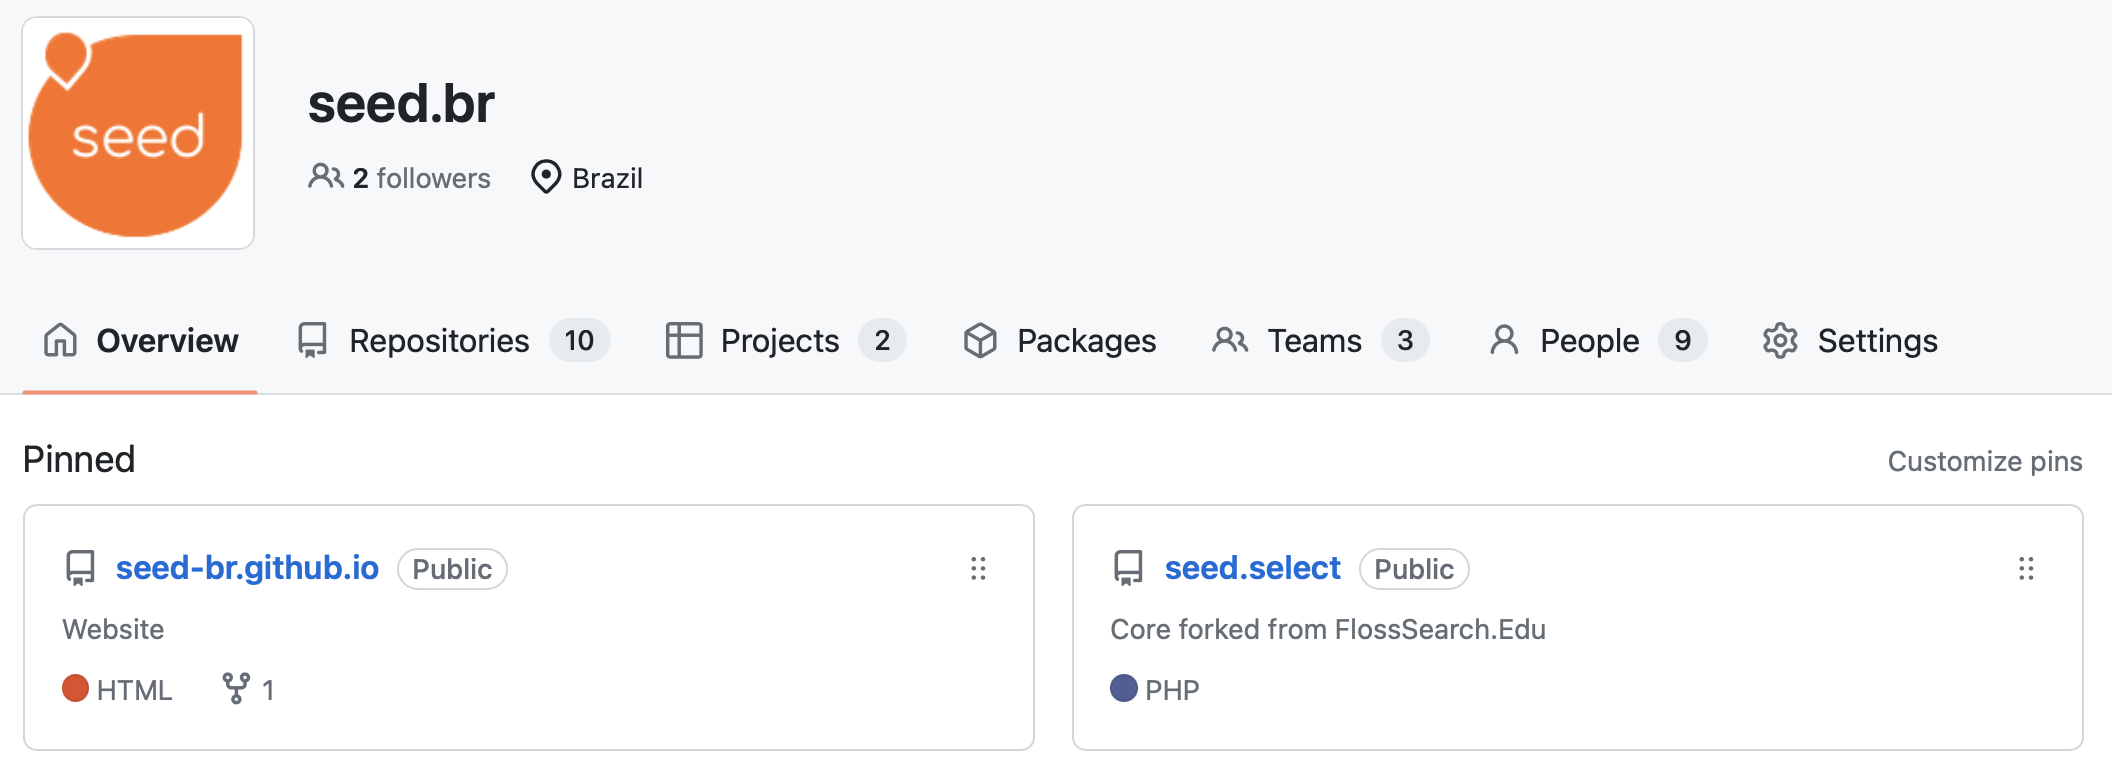
\includegraphics[scale=0.40]{JAI 2023/figures/seed-organization.png}
    \caption{Organização seed.br e repositório seed.select no GitHub.}
    \label{fig:hospedagem:seed}
\end{figure}

\noindent \textbf{\texttt{seed.select}}.
A primeiro lançamento do software ... versão 1.0.0 ...
A Figura~\ref{fig:seed-select-release} mostra ...

\begin{figure}[htb]
    \centering
    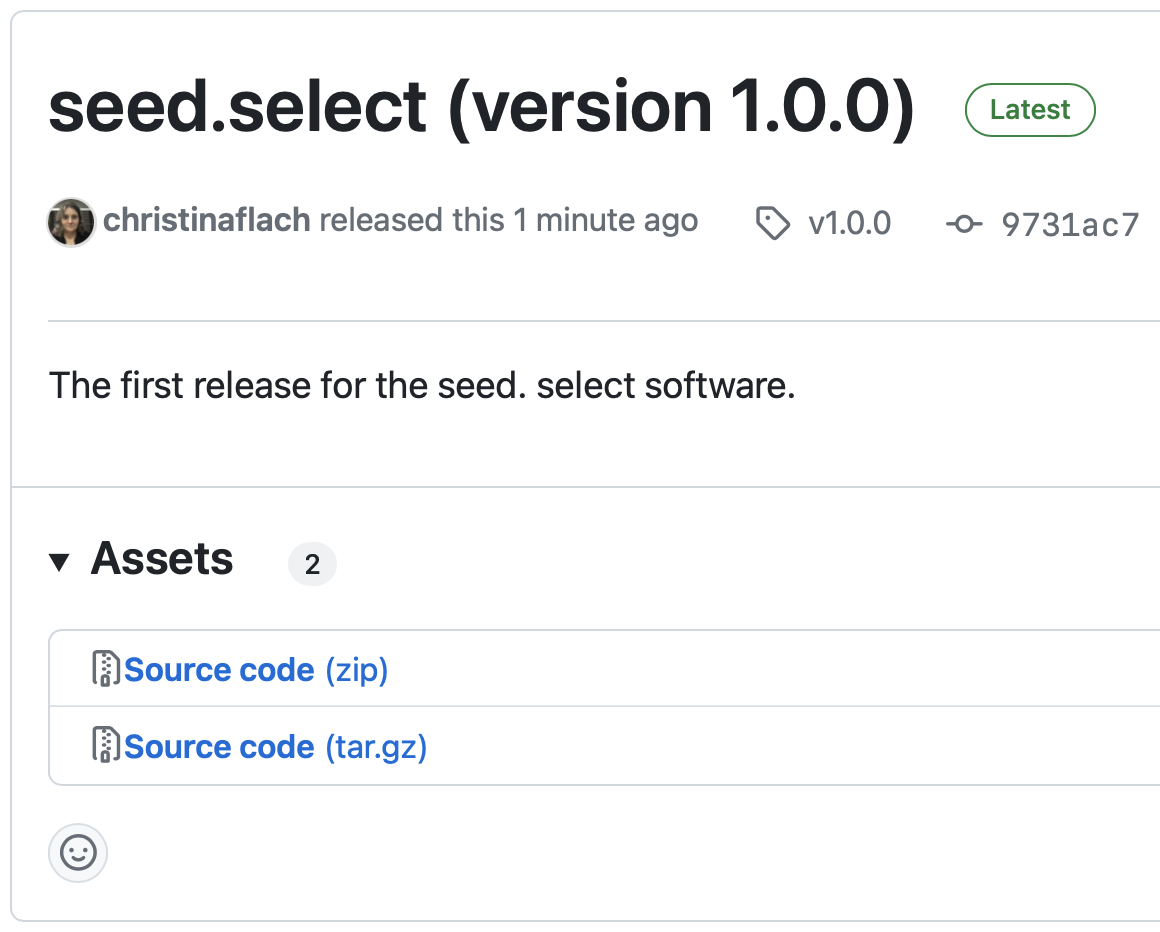
\includegraphics[scale=0.5]{JAI 2023/figures/seed-select-release-v1.0.0.png}
    \caption{Release v1.0.0}
    \label{fig:seed-select-release}
\end{figure}

\noindent \textbf{\texttt{seed.select}}.
O software não possui um PID mas possui uma versão e um identificador (URL).
Para citá-lo, atribuímos a autoria ao projeto de pesquisa no qual o software de pesquisa foi delineado e desenvolvido. 
Os nomes dos contribuidores aparecem listados no arquivo AUTHORS.md.

\begin{quote}
    SEED.BR Project (2020). seed.select (version 1.0.0) [Computer software] https://github.com/seed-br/seed.select/releases/tag/v1.0.0
\end{quote}

\noindent \textbf{\texttt{seed.select}}.
A definição de testes e uso de automação de teses foram registradas como prioritárias no kanbam do projeto.

\noindent \textbf{\texttt{seed.select}}.
O uso de ferramentas de CI/CD no desenvolvimento do
software de pesquisa X foi registrado no kanbam do projeto.

\subsection*{Avaliação da Sustentabilidade}

%\input{JAI 2023/tables/ssi-criteria-seed}

\subsection*{Avaliação de \textit{FAIRness}}

%\input{JAI 2023/tables/fairness-seed}


\subsection{Próximos passos}

\subsection{Convite para contribuir}



% The purpose of basic research is to understand and explain.
% An example within reasearch software is to understand why researchers develop they own software and which software engineering practices they use. The basic researcher has to look into the researcher (subject) thoughts and research software to find out ...
%\section{Autores}
\subsection*{Christina von Flach Garcia Chavez}
    \begin{itemize}
        \item E-mail para contato: flach@ufba.br
%        \item Número de associado: 8925
        \item Instituição: Universidade Federal da Bahia (UFBA)
        \item Mini-bio: Christina von Flach é Professora Associada do Instituto de Computação da UFBA. Seus interesses de pesquisa incluem aspectos sócio-técnicos de ecossistemas de software, sustentabilidade do software, software livre e educação em engenharia de software. Co-organizou o I Workshop sobre Práticas de Ciência Aberta na pesquisa em Engenharia de Software, realizado durante o CBSOFT'21. Coordena os \textit{Seminários sobre Desafios e Práticas da Ciência Aberta na Computação} em parceria com a Prof. Claudia Maria Bauzer de Medeiros, evento-satélite do CSBC 2023. Lecionou cursos de pós-graduação com um subconjunto da temática deste curso em quatro ocasiões. Orientou a primeira dissertação de mestrado no Brasil sobre o tema deste curso, ``Sustentabilidade técnica de software acadêmico no domínio de ferramentas de análise estática'', defendida por um dos co-autores. Atualmente, é orientadora da pesquisa de mestrado de Daniela Feitosa (co-autora) sobre este tema.
        \end{itemize}

\subsection*{Joenio Marques da Costa}
    \begin{itemize}
        \item E-mail para contato: joenio@joenio.me
        \item Instituição: Université Gustave Eiffel (UGE)
        \item Mini-bio: Joenio M. Costa é engenheiro de \textit{software de pesquisa} (Research Software Engineer) no laboratorio LISIS (Laboratoire Interdisciplinaire Sciences Innovations Sociétés), trabalhando como desenvolvedor \textit{backend} nos projetos RISIS (Research Infrastructure for Science, technology and Innovation policy Studies) e CorTexT. Seus interesses de pesquisas incluem sustentabilidade de software, software de pesquisa, citação de software e qualidade de software. É colaborador do sistema operacional livre Debian, instrutor de Computação no \textit{The Carpentries} e embaixador do \textit{Sofware Heritage}, o arquivo universal de preservação de código fonte de software.
    \end{itemize}

\subsection*{Daniela Soares Feitosa}
    \begin{itemize}
        \item E-mail para contato: danielafeitosa@gmail.com
        \item Instituição: Universidade Federal da Bahia (UFBA)
        \item Mini-bio: Daniela Feitosa é engenheira de software e estudante de mestrado
        no Programa de Pós-graduação em Ciência da Computação (PGCOMP) na Universidade Federal da Bahia (UFBA). Seus interesses de pesquisa incluem sustentabilidade do software, software livre, qualidade de software e educação em engenharia de software. Seu projeto de pesquisa no Mestrado está alinhado com os objetivos deste curso.    
    \end{itemize}

\end{document}
